%%%%%%%%%%%%%%%%%%%%%%%%%%%%%%%%%%%%%%%%%
% Masters/Doctoral Thesis
% LaTeX Template (Version 2.5, 27/8/17)
% http://www.LaTeXTemplates.com  --  Vel (vel@latextemplates.com)
% Based on templates by Steve Gunn and Sunil Patel.
% License: CC BY-NC-SA 3.0
%%%%%%%%%%%%%%%%%%%%%%%%%%%%%%%%%%%%%%%%%


% Alternative title-page branding is retained under Figures/branding/.

%----------------------------------------------------------------------------------------
%	PACKAGES AND OTHER DOCUMENT CONFIGURATIONS
%----------------------------------------------------------------------------------------

\documentclass[
11pt, % The default document font size, options: 10pt, 11pt, 12pt
oneside, % Two side (alternating margins) for binding by default, uncomment to switch to one side
english, % ngerman for German
singlespacing, % Single line spacing, alternatives: onehalfspacing or doublespacing
%draft, % Uncomment to enable draft mode (no pictures, no links, overfull hboxes indicated)
%nolistspacing, % If the document is onehalfspacing or doublespacing, uncomment this to set spacing in lists to single
%liststotoc, % Uncomment to add the list of figures/tables/etc to the table of contents
%toctotoc, % Uncomment to add the main table of contents to the table of contents
parskip, % Uncomment to add space between paragraphs
%nohyperref, % Uncomment to not load the hyperref package
headsepline, % Uncomment to get a line under the header
%chapterinoneline, % Uncomment to place the chapter title next to the number on one line
%consistentlayout, % Uncomment to change the layout of the declaration, abstract and acknowledgements pages to match the default layout
]{MastersDoctoralThesis} % The class file specifying the document structure

\usepackage{iftex}
\ifPDFTeX
  \usepackage[utf8]{inputenc} % Required for inputting international characters
  \usepackage[T1]{fontenc} % Output font encoding for international characters
  \usepackage{lmodern} % Latin Modern — the standard LaTeX font, with real small caps
\else % XeLaTeX / LuaLaTeX
  \usepackage{fontspec} % also defaults to Latin Modern
\fi
\usepackage{microtype} % finer justification (protrusion + font expansion under pdflatex)

% sorting=none is load-bearing: biblatex's numeric styles default to sorting=nty
% (alphabetical by author), which numbers the bibliography down a sorted list rather
% than by first appearance. Without it, adding a reference that sorts early shifts
% every later citation number.
% backend=biber is load-bearing too. Under backend=bibtex, BibTeX runs with its working
% directory set to the latexmk output directory (build/) and cannot resolve references.bib
% one level up, so every \cite silently fell back to [key] with "I didn't find a database
% entry" in build/main.blg. Biber resolves \addbibresource relative to the main .tex, so the
% out-of-tree build works. Do not switch this back without also fixing BIBINPUTS.
\usepackage[backend=biber,style=numeric-comp,sorting=none,natbib=false]{biblatex} % Numeric-comp, numbered in order of first citation

\addbibresource{references.bib} % The filename of the bibliography

\usepackage[autostyle=true]{csquotes} % Required to generate language-dependent quotes in the bibliography

\usepackage{amsthm}
\usepackage{algorithm} % float environment for pseudo-code
\usepackage{algpseudocode} % algorithmicx pseudo-code body
\newtheorem{theorem}{Theorem}

\usepackage{pdfpages}

% Scientific figures are exported as title-free PDF panels. LaTeX owns panel
% letters, panel descriptions and the overall caption so typography remains
% readable and consistent at the final A4 text width.
\usepackage{subcaption}

% Floats are declared [tbp] so they never split a paragraph, but that alone lets them
% drift past the section they belong to -- Table 3.1 was landing inside Section 3.2.
% The [section] option issues a \FloatBarrier before every \section, so a float must
% be placed before the next section begins. Result: no float breaks running text, and
% no float escapes its own section.
\usepackage[section]{placeins}

%----------------------------------------------------------------------------------------
%	IMPERIAL COLOUR PALETTE
%	xcolor is already loaded by MastersDoctoralThesis.cls (with dvipsnames).
%	Names below match Imperial's supplied swatches; reuse them in tables, tikz,
%	and (mirrored in Python) for figures.
%----------------------------------------------------------------------------------------

% ---- Primary ----
\definecolor{ImperialBlue}{HTML}{0000CD}   % headline colour
\definecolor{ImperialNavy}{HTML}{000080}
\definecolor{ImperialDark}{HTML}{232333}

% ---- Extended palette ----
\definecolor{ImpSaddleBrown}{HTML}{8B4513}
\definecolor{ImpTeal}{HTML}{008080}
\definecolor{ImpVioletRed}{HTML}{C71585}
\definecolor{ImpIndigo}{HTML}{4B0082}
\definecolor{ImpCrimson}{HTML}{DC143C}
\definecolor{ImpOrangeRed}{HTML}{FF4500}
\definecolor{ImpDarkGreen}{HTML}{006400}
\definecolor{ImpSlateGray}{HTML}{708090}
\definecolor{ImpYellow}{HTML}{FFFF00}
\definecolor{ImpTurquoise}{HTML}{40E0D0}
\definecolor{ImpViolet}{HTML}{EE82EE}
\definecolor{ImpMediumSlateBlue}{HTML}{7B68EE}
\definecolor{ImpRed}{HTML}{FF0000}
\definecolor{ImpDarkOrange}{HTML}{FF8C00}
\definecolor{ImpSpringGreen}{HTML}{00FF7F}
\definecolor{ImpWhiteSmoke}{HTML}{F5F5F5}
\definecolor{ImpDeepSkyBlue}{HTML}{00BFFF}
\definecolor{ImpKhaki}{HTML}{F0E68C}
\definecolor{ImpPaleTurquoise}{HTML}{AFEEEE}
\definecolor{ImpLightPink}{HTML}{FFB6C1}
\definecolor{ImpLavender}{HTML}{E6E6FA}
\definecolor{ImpSalmon}{HTML}{FA8072}
\definecolor{ImpOrange}{HTML}{FFA500}
\definecolor{ImpPaleGreen}{HTML}{98FB98}

%----------------------------------------------------------------------------------------
%	HEADINGS IN IMPERIAL BLUE
%----------------------------------------------------------------------------------------

% Chapter titles use the class's own hooks (see MastersDoctoralThesis.cls).
\RenewDocumentCommand{\chapterfont}{}{\Huge\bfseries\color{ImperialBlue}}
\RenewDocumentCommand{\chapterprefixfont}{}{\LARGE\bfseries\color{ImperialBlue}}

% Section levels: replicate the book-class defaults and add \color, so spacing is
% untouched and no sectioning package (titlesec/sectsty) is needed.
\makeatletter
\renewcommand\section{\@startsection{section}{1}{\z@}%
  {-3.5ex \@plus -1ex \@minus -.2ex}{2.3ex \@plus.2ex}%
  {\normalfont\Large\bfseries\color{ImperialBlue}}}
\renewcommand\subsection{\@startsection{subsection}{2}{\z@}%
  {-3.25ex\@plus -1ex \@minus -.2ex}{1.5ex \@plus .2ex}%
  {\normalfont\large\bfseries\color{ImperialBlue}}}
\renewcommand\subsubsection{\@startsection{subsubsection}{3}{\z@}%
  {-3.25ex\@plus -1ex \@minus -.2ex}{1.5ex \@plus .2ex}%
  {\normalfont\normalsize\bfseries\color{ImperialBlue}}}
\makeatother

% Title-page rules in Imperial Blue.
\renewcommand{\HRule}{\textcolor{ImperialBlue}{\rule{\linewidth}{0.6pt}}}
\renewcommand{\decoRule}{\textcolor{ImperialBlue}{\rule{.8\textwidth}{.4pt}}}

%----------------------------------------------------------------------------------------
%	HYPERLINK COLOURS (override the class defaults at end of preamble)
%----------------------------------------------------------------------------------------
% hyperref has a single knob for internal cross-references: linkcolor covers figure, table,
% section, equation and table-of-contents links alike, so making figure/table numbers black
% necessarily makes every internal reference black. Citations and URLs keep their colour.
\AtBeginDocument{\hypersetup{
  linkcolor=black,          % internal refs (figures, tables, sections, equations, ToC)
  citecolor=ImperialNavy,   % citations
  urlcolor=ImperialBlue,    % URLs
}}
 % Imperial colour palette + headings/links in Imperial Blue

% Figure numbers quoted in captions, generated alongside the figures themselves by
% dissertation/scripts/generate_hu_imbalance_histogram.py. Keeping them in a
% generated file rather than typed into the caption means the prose cannot drift
% from the plot when the cohort or the generation split changes.
% GENERATED by dissertation/scripts/generate_hu_imbalance_histogram.py.
% Do not edit: re-run the script instead, so the caption and the plot stay
% in agreement. Negative HU values are wrapped for math mode by the caller.
\newcommand{\airwayNcases}{260}
\newcommand{\airwayFgRoi}{0.29}
\newcommand{\airwayFgVolume}{0.092}
\newcommand{\airwayProxBranchShare}{4.0}
\newcommand{\airwayProxVoxelShare}{65.0}
\newcommand{\airwayProxMedianHU}{-980}
\newcommand{\airwayDistMedianHU}{-912}
\newcommand{\airwayParenMedianHU}{-870}
\newcommand{\airwayGenZeroPerCase}{1.0}
\newcommand{\airwayGenOnePerCase}{2.2}
\newcommand{\airwayGenTwoPerCase}{4.8}
\newcommand{\airwayProximalMaxGen}{2}


% Measured airway calibres quoted in the opening figure's caption, generated by
% dissertation/scripts/generate_intro_airway_overview.py alongside the panels
% themselves. Same contract: the caption cannot drift from the artwork.
% GENERATED by dissertation/scripts/generate_intro_airway_overview.py.
% Do not edit: re-run the script instead, so the caption and the panel stay
% in agreement. Each diameter is the largest inscribed in-plane circle within
% that inset box, which equals the true local calibre for a tube cut at any
% obliquity rather than an inflated oblique width.
\newcommand{\airwayTracheaDiameter}{15}
\newcommand{\airwayDistalDiameter}{2.6}
\newcommand{\airwayInsetBox}{30}
\newcommand{\airwayInsetScaleBar}{5}


% Placeholder marker for results that are computed but not yet scored, or still
% training. It renders in red so it cannot survive a proof-read by accident, and
% every outstanding item is findable with one search for "\pending".
% BEFORE SUBMISSION: grep for \pending; the document must contain none.
\newcommand{\pending}[1][]{%
  \textcolor{red}{\textbf{[pending#1]}}%
}

% Alternative primary-control narratives. The working draft shows both: blue is the
% currently scored fitted-checkpoint comparison and red is the prospective paired-seed
% comparison. Before submission set exactly one switch to true.
\newif\ifshowcurrentcontrol
\newif\ifshowpairedcontrol
\showcurrentcontroltrue
\showpairedcontroltrue
\newenvironment{currentcontrolroute}{\begingroup\color{ImperialBlue}}{\endgroup}
\newenvironment{pairedcontrolroute}{\begingroup\color{ImpRed}}{\endgroup}

% Paired-test statistics, generated by dissertation/scripts/statistics/
% paired_significance_tests.py. Quoting these macros in prose rather than typing the
% numbers means a significance claim in the text cannot drift from Table~\ref{tab:paired-tests}.
% GENERATED by dissertation/scripts/statistics/paired_significance_tests.py.
% Do not edit. Use e.g. \statTestSoftCtrlTLDDiff in prose so the number in the
% text can never drift from the number in the table.
\newcommand{\statValSoftCtrlDiceDiff}{-0.0039}
\newcommand{\statValSoftCtrlDiceT}{-2.17}
\newcommand{\statValSoftCtrlDiceP}{0.2139}
\newcommand{\statValSoftCtrlDiceWins}{7/20}
\newcommand{\statValSoftCtrlTLDDiff}{+0.0196}
\newcommand{\statValSoftCtrlTLDT}{+8.42}
\newcommand{\statValSoftCtrlTLDP}{<10^{-4}}
\newcommand{\statValSoftCtrlTLDWins}{20/20}
\newcommand{\statValSoftCtrlBDDiff}{+0.0362}
\newcommand{\statValSoftCtrlBDT}{+5.84}
\newcommand{\statValSoftCtrlBDP}{<10^{-4}}
\newcommand{\statValSoftCtrlBDWins}{19/20}
\newcommand{\statValSoftCtrlPrecDiff}{+0.0057}
\newcommand{\statValSoftCtrlPrecT}{+1.66}
\newcommand{\statValSoftCtrlPrecP}{0.5647}
\newcommand{\statValSoftCtrlPrecWins}{13/20}
\newcommand{\statValSoftCtrlclDiceDiff}{-0.0012}
\newcommand{\statValSoftCtrlclDiceT}{-0.48}
\newcommand{\statValSoftCtrlclDiceP}{1.0000}
\newcommand{\statValSoftCtrlclDiceWins}{9/20}
\newcommand{\statValHardCtrlDiceDiff}{+0.0041}
\newcommand{\statValHardCtrlDiceT}{+0.91}
\newcommand{\statValHardCtrlDiceP}{1.0000}
\newcommand{\statValHardCtrlDiceWins}{14/20}
\newcommand{\statValHardCtrlTLDDiff}{+0.0190}
\newcommand{\statValHardCtrlTLDT}{+10.47}
\newcommand{\statValHardCtrlTLDP}{<10^{-4}}
\newcommand{\statValHardCtrlTLDWins}{20/20}
\newcommand{\statValHardCtrlBDDiff}{+0.0348}
\newcommand{\statValHardCtrlBDT}{+6.27}
\newcommand{\statValHardCtrlBDP}{<10^{-4}}
\newcommand{\statValHardCtrlBDWins}{20/20}
\newcommand{\statValHardCtrlPrecDiff}{+0.0154}
\newcommand{\statValHardCtrlPrecT}{+2.72}
\newcommand{\statValHardCtrlPrecP}{0.0683}
\newcommand{\statValHardCtrlPrecWins}{17/20}
\newcommand{\statValHardCtrlclDiceDiff}{+0.0051}
\newcommand{\statValHardCtrlclDiceT}{+2.80}
\newcommand{\statValHardCtrlclDiceP}{0.0576}
\newcommand{\statValHardCtrlclDiceWins}{14/20}
\newcommand{\statValHardCeilDiceDiff}{+0.0055}
\newcommand{\statValHardCeilDiceT}{+1.53}
\newcommand{\statValHardCeilDiceP}{0.7166}
\newcommand{\statValHardCeilDiceWins}{13/20}
\newcommand{\statValHardCeilTLDDiff}{+0.0059}
\newcommand{\statValHardCeilTLDT}{+2.45}
\newcommand{\statValHardCeilTLDP}{0.1205}
\newcommand{\statValHardCeilTLDWins}{14/20}
\newcommand{\statValHardCeilBDDiff}{+0.0079}
\newcommand{\statValHardCeilBDT}{+1.62}
\newcommand{\statValHardCeilBDP}{0.6139}
\newcommand{\statValHardCeilBDWins}{12/20}
\newcommand{\statValHardCeilPrecDiff}{+0.0020}
\newcommand{\statValHardCeilPrecT}{+0.31}
\newcommand{\statValHardCeilPrecP}{1.0000}
\newcommand{\statValHardCeilPrecWins}{8/20}
\newcommand{\statValHardCeilclDiceDiff}{-0.0004}
\newcommand{\statValHardCeilclDiceT}{-0.21}
\newcommand{\statValHardCeilclDiceP}{1.0000}
\newcommand{\statValHardCeilclDiceWins}{9/20}
\newcommand{\statValBetaSoftDiceDiff}{-0.0743}
\newcommand{\statValBetaSoftDiceT}{-2.15}
\newcommand{\statValBetaSoftDiceP}{0.2228}
\newcommand{\statValBetaSoftDiceWins}{5/20}
\newcommand{\statValBetaSoftTLDDiff}{+0.0230}
\newcommand{\statValBetaSoftTLDT}{+3.94}
\newcommand{\statValBetaSoftTLDP}{0.0044}
\newcommand{\statValBetaSoftTLDWins}{18/20}
\newcommand{\statValBetaSoftBDDiff}{+0.0475}
\newcommand{\statValBetaSoftBDT}{+3.45}
\newcommand{\statValBetaSoftBDP}{0.0133}
\newcommand{\statValBetaSoftBDWins}{16/20}
\newcommand{\statValBetaSoftPrecDiff}{-0.1357}
\newcommand{\statValBetaSoftPrecT}{-3.12}
\newcommand{\statValBetaSoftPrecP}{0.0280}
\newcommand{\statValBetaSoftPrecWins}{0/20}
\newcommand{\statValBetaSoftclDiceDiff}{-0.1823}
\newcommand{\statValBetaSoftclDiceT}{-3.58}
\newcommand{\statValBetaSoftclDiceP}{0.0100}
\newcommand{\statValBetaSoftclDiceWins}{0/20}
\newcommand{\statTestSoftCtrlDiceDiff}{-0.0008}
\newcommand{\statTestSoftCtrlDiceT}{-0.35}
\newcommand{\statTestSoftCtrlDiceP}{1.0000}
\newcommand{\statTestSoftCtrlDiceWins}{10/20}
\newcommand{\statTestSoftCtrlTLDDiff}{+0.0181}
\newcommand{\statTestSoftCtrlTLDT}{+6.90}
\newcommand{\statTestSoftCtrlTLDP}{<10^{-4}}
\newcommand{\statTestSoftCtrlTLDWins}{19/20}
\newcommand{\statTestSoftCtrlBDDiff}{+0.0379}
\newcommand{\statTestSoftCtrlBDT}{+6.85}
\newcommand{\statTestSoftCtrlBDP}{<10^{-4}}
\newcommand{\statTestSoftCtrlBDWins}{19/20}
\newcommand{\statTestSoftCtrlPrecDiff}{+0.0104}
\newcommand{\statTestSoftCtrlPrecT}{+2.64}
\newcommand{\statTestSoftCtrlPrecP}{0.0813}
\newcommand{\statTestSoftCtrlPrecWins}{14/20}
\newcommand{\statTestSoftCtrlclDiceDiff}{-0.0016}
\newcommand{\statTestSoftCtrlclDiceT}{-0.67}
\newcommand{\statTestSoftCtrlclDiceP}{1.0000}
\newcommand{\statTestSoftCtrlclDiceWins}{8/20}
\newcommand{\statTestHardCtrlDiceDiff}{+0.0116}
\newcommand{\statTestHardCtrlDiceT}{+3.71}
\newcommand{\statTestHardCtrlDiceP}{0.0074}
\newcommand{\statTestHardCtrlDiceWins}{16/20}
\newcommand{\statTestHardCtrlTLDDiff}{+0.0143}
\newcommand{\statTestHardCtrlTLDT}{+6.43}
\newcommand{\statTestHardCtrlTLDP}{<10^{-4}}
\newcommand{\statTestHardCtrlTLDWins}{20/20}
\newcommand{\statTestHardCtrlBDDiff}{+0.0300}
\newcommand{\statTestHardCtrlBDT}{+5.85}
\newcommand{\statTestHardCtrlBDP}{<10^{-4}}
\newcommand{\statTestHardCtrlBDWins}{18/20}
\newcommand{\statTestHardCtrlPrecDiff}{+0.0233}
\newcommand{\statTestHardCtrlPrecT}{+3.90}
\newcommand{\statTestHardCtrlPrecP}{0.0048}
\newcommand{\statTestHardCtrlPrecWins}{19/20}
\newcommand{\statTestHardCtrlclDiceDiff}{+0.0017}
\newcommand{\statTestHardCtrlclDiceT}{+0.59}
\newcommand{\statTestHardCtrlclDiceP}{1.0000}
\newcommand{\statTestHardCtrlclDiceWins}{13/20}
\newcommand{\statTestHardCeilDiceDiff}{+0.0067}
\newcommand{\statTestHardCeilDiceT}{+1.12}
\newcommand{\statTestHardCeilDiceP}{1.0000}
\newcommand{\statTestHardCeilDiceWins}{11/20}
\newcommand{\statTestHardCeilTLDDiff}{+0.0037}
\newcommand{\statTestHardCeilTLDT}{+1.36}
\newcommand{\statTestHardCeilTLDP}{0.9466}
\newcommand{\statTestHardCeilTLDWins}{14/20}
\newcommand{\statTestHardCeilBDDiff}{+0.0140}
\newcommand{\statTestHardCeilBDT}{+2.48}
\newcommand{\statTestHardCeilBDP}{0.1133}
\newcommand{\statTestHardCeilBDWins}{15/20}
\newcommand{\statTestHardCeilPrecDiff}{+0.0145}
\newcommand{\statTestHardCeilPrecT}{+1.29}
\newcommand{\statTestHardCeilPrecP}{1.0000}
\newcommand{\statTestHardCeilPrecWins}{11/20}
\newcommand{\statTestHardCeilclDiceDiff}{-0.0037}
\newcommand{\statTestHardCeilclDiceT}{-1.43}
\newcommand{\statTestHardCeilclDiceP}{0.8459}
\newcommand{\statTestHardCeilclDiceWins}{8/20}
\newcommand{\statTestBetaCtrlDiceDiff}{-0.0575}
\newcommand{\statTestBetaCtrlDiceT}{-3.91}
\newcommand{\statTestBetaCtrlDiceP}{0.0047}
\newcommand{\statTestBetaCtrlDiceWins}{0/20}
\newcommand{\statTestBetaCtrlTLDDiff}{+0.0348}
\newcommand{\statTestBetaCtrlTLDT}{+8.80}
\newcommand{\statTestBetaCtrlTLDP}{<10^{-4}}
\newcommand{\statTestBetaCtrlTLDWins}{20/20}
\newcommand{\statTestBetaCtrlBDDiff}{+0.0654}
\newcommand{\statTestBetaCtrlBDT}{+8.14}
\newcommand{\statTestBetaCtrlBDP}{<10^{-4}}
\newcommand{\statTestBetaCtrlBDWins}{20/20}
\newcommand{\statTestBetaCtrlPrecDiff}{-0.1097}
\newcommand{\statTestBetaCtrlPrecT}{-5.10}
\newcommand{\statTestBetaCtrlPrecP}{0.0003}
\newcommand{\statTestBetaCtrlPrecWins}{0/20}
\newcommand{\statTestBetaCtrlclDiceDiff}{-0.1503}
\newcommand{\statTestBetaCtrlclDiceT}{-4.19}
\newcommand{\statTestBetaCtrlclDiceP}{0.0025}
\newcommand{\statTestBetaCtrlclDiceWins}{0/20}
\newcommand{\statOodSoftCtrlDiceDiff}{+0.0002}
\newcommand{\statOodSoftCtrlDiceT}{+0.06}
\newcommand{\statOodSoftCtrlDiceP}{1.0000}
\newcommand{\statOodSoftCtrlDiceWins}{16/27}
\newcommand{\statOodSoftCtrlTLDDiff}{+0.0057}
\newcommand{\statOodSoftCtrlTLDT}{+2.59}
\newcommand{\statOodSoftCtrlTLDP}{0.0774}
\newcommand{\statOodSoftCtrlTLDWins}{17/27}
\newcommand{\statOodSoftCtrlBDDiff}{+0.0132}
\newcommand{\statOodSoftCtrlBDT}{+3.00}
\newcommand{\statOodSoftCtrlBDP}{0.0297}
\newcommand{\statOodSoftCtrlBDWins}{15/27}
\newcommand{\statOodSoftCtrlPrecDiff}{+0.0143}
\newcommand{\statOodSoftCtrlPrecT}{+2.71}
\newcommand{\statOodSoftCtrlPrecP}{0.0581}
\newcommand{\statOodSoftCtrlPrecWins}{20/27}
\newcommand{\statOodSoftCtrlclDiceDiff}{-0.0232}
\newcommand{\statOodSoftCtrlclDiceT}{-3.81}
\newcommand{\statOodSoftCtrlclDiceP}{0.0038}
\newcommand{\statOodSoftCtrlclDiceWins}{4/27}
\newcommand{\statOodHardCeilDiceDiff}{-0.0043}
\newcommand{\statOodHardCeilDiceT}{-0.99}
\newcommand{\statOodHardCeilDiceP}{1.0000}
\newcommand{\statOodHardCeilDiceWins}{9/27}
\newcommand{\statOodHardCeilTLDDiff}{+0.0053}
\newcommand{\statOodHardCeilTLDT}{+2.85}
\newcommand{\statOodHardCeilTLDP}{0.0423}
\newcommand{\statOodHardCeilTLDWins}{23/27}
\newcommand{\statOodHardCeilBDDiff}{+0.0034}
\newcommand{\statOodHardCeilBDT}{+1.36}
\newcommand{\statOodHardCeilBDP}{0.9198}
\newcommand{\statOodHardCeilBDWins}{11/27}
\newcommand{\statOodHardCeilPrecDiff}{-0.0177}
\newcommand{\statOodHardCeilPrecT}{-9.00}
\newcommand{\statOodHardCeilPrecP}{<10^{-4}}
\newcommand{\statOodHardCeilPrecWins}{1/27}
\newcommand{\statOodHardCeilclDiceDiff}{-0.0279}
\newcommand{\statOodHardCeilclDiceT}{-7.47}
\newcommand{\statOodHardCeilclDiceP}{<10^{-4}}
\newcommand{\statOodHardCeilclDiceWins}{2/27}


%----------------------------------------------------------------------------------------
%	FLOAT PLACEMENT
%----------------------------------------------------------------------------------------
% LaTeX's defaults are tuned for a book with far more text than figures, and in a
% 6,000-word report with up to 20 figures they strand floats on pages of their own.
% Figure 1.2 is only ~47% of the text height and was still being banished to a
% dedicated float page surrounded by whitespace.
%
% topfraction/bottomfraction: how much of a TEXT page a float may occupy. Raised, so
%   a half-page figure can still share a page with prose.
% textfraction: how little text a page may carry before LaTeX gives up on it. Lowered.
% floatpagefraction: how full a FLOAT-ONLY page must be to be allowed. RAISED, which
%   is the parameter that actually suppresses near-empty float pages -- a float now has
%   to fill 80% of a page before it is granted one. Must stay below topfraction.
\renewcommand{\topfraction}{0.9}
\renewcommand{\bottomfraction}{0.7}
\renewcommand{\textfraction}{0.1}
\renewcommand{\floatpagefraction}{0.8}
\setcounter{topnumber}{3}
\setcounter{bottomnumber}{2}
\setcounter{totalnumber}{4}

%----------------------------------------------------------------------------------------
%	MARGIN SETTINGS
%----------------------------------------------------------------------------------------

\geometry{
	paper=a4paper, % Change to letterpaper for US letter
	top=2.54cm, % Top margin (official Imperial template)
	bottom=2.54cm, % Bottom margin
	left=1.91cm, % Symmetric margins for electronic submission (no binding offset)
	right=1.91cm, % Right margin
    %showframe, % Uncomment to show how the type block is set on the page
}

%----------------------------------------------------------------------------------------
%	THESIS INFORMATION
%----------------------------------------------------------------------------------------

% TODO: confirm the final title, supervisor, degree programme and department below.
\thesistitle{Can Mean Teacher Learning Recover Missing Airway Branches? A Topology-Aware Study of Semi-Supervised Pulmonary Airway Segmentation in CT} % Provisional working title; print with \ttitle
\supervisor{Dr Guang \textsc{Yang}} % Dept booklet lists "Dr Yang, Guang" — change to Prof. if updated
\examiner{} % Your examiner's name (not used by default); print with \examname
\degree{MSc TODO} % Your degree/programme name; print with \degreename
\author{Daniel \textsc{Lucas}} % Your name; print with \authorname
\addresses{} % Not used by default; print with \addressname

\subject{Semi-Supervised Medical Image Segmentation} % Not used by default; print with \subjectname
\keywords{Mean Teacher; semi-supervised learning; airway segmentation; topology-aware evaluation; clDice; nnU-Net} % Not used by default; print with \keywordnames
\university{\href{https://www.imperial.ac.uk}{Imperial College London}} % Print with \univname
\department{\href{https://www.imperial.ac.uk/bioengineering/}{Department of Bioengineering}} % Print with \deptname
\group{} % Print with \groupname
\faculty{\href{https://www.imperial.ac.uk/engineering/}{Faculty of Engineering}} % Print with \facname

\AtBeginDocument{
\hypersetup{pdftitle=\ttitle} % Set the PDF's title to your title
\hypersetup{pdfauthor=\authorname} % Set the PDF's author to your name
\hypersetup{pdfkeywords=\keywordnames} % Set the PDF's keywords to your keywords
}

\begin{document}

\frontmatter % Use roman page numbering style (i, ii, iii, iv...) for the pre-content pages

\pagestyle{plain} % Default to the plain heading style until the thesis style is called for the body content

\newtheorem{definition}{Definition}
\newtheorem{remark}{Remark}

%----------------------------------------------------------------------------------------
%	TITLE PAGE
%----------------------------------------------------------------------------------------

%TC:ignore  (front matter below is excluded from the 6000-word body count)
\begin{titlepage}
\begin{center}

\vspace*{.06\textheight}
{\scshape\LARGE \univname\par} % University name
\vspace{0.8cm}
% \textsc{\Large \facname}\vspace{0.6cm} % Faculty

% Imperial logo on the title page only. PDF is preferred when supplied; the
% organised PNG fallback below keeps the document compilable in this workspace.
\IfFileExists{Figures/branding/imperial_logo_blue_2024.pdf}
  {
\includegraphics[width=0.65\textwidth]{Figures/branding/imperial_logo_blue_2024.pdf}\par\vspace{0.6cm}}
  {\IfFileExists{Figures/branding/imperial_logo_blue_2024.png}
    {
\includegraphics[width=0.65\textwidth]{Figures/branding/imperial_logo_blue_2024.png}\par\vspace{0.6cm}}
    {}}

\textsc{\Large MSc Individual Project}\\[0.5cm] % Document type
\HRule \\[0.4cm] % Horizontal line
{\huge \bfseries \ttitle\par}\vspace{0.4cm} % Thesis title
\HRule \\[1.5cm] % Horizontal line

\textsc{\Large \deptname}\\[0.5cm] % Department

\begin{minipage}[t]{0.4\textwidth}
\begin{flushleft} \large
\emph{Author:}\\
{\authorname} \\ % Author name
CID: 06059393
\end{flushleft}
\end{minipage}
\begin{minipage}[t]{0.4\textwidth}
\begin{flushright} \large
\emph{Supervisor:} \\
\supname
\end{flushright}
\end{minipage}\\[3cm]

\vfill

%{\large A dissertation submitted in partial fulfilment of the requirements for the degree of \degreename}\\[0.3cm]
{\large \today}\\[4cm] % Date

\end{center}
\end{titlepage}

%----------------------------------------------------------------------------------------
%	ABSTRACT PAGE
%----------------------------------------------------------------------------------------

\begin{abstract}
\addchaptertocentry{\abstractname} % Add the abstract to the table of contents
% ROUGH-DRAFT NOTE: replace this list with a single paragraph, <=250 words (hard limit),
% once the soft-clDice arm and its matched control have been scored on VAL20.
\begin{itemize}
  \item \textbf{Problem:} voxel-level airway annotation is expensive while unlabelled
  thoracic CT is abundant; the distal tree is where segmentation fails and where volumetric
  Dice is least able to see the failure.
  \item \textbf{Question:} can teacher-derived consistency on unlabelled scans recover
  branches that a label-starved teacher omits, or does it only consolidate structure the
  teacher already predicts?
  \item \textbf{Approach:} Mean Teacher on nnU-Net with geometry-aware (soft-clDice)
  consistency, against an \emph{exactly matched} no-consistency continuation --- same warm
  start, schedule, sampler, perturbation, optimiser steps and EMA deployment, removing only
  the unlabelled gradient.
  \par\textcolor{red}{\textbf{This should be changed to:} Mean Teacher with geometry-aware
  consistency compared with a \emph{configuration-matched} no-consistency continuation. The
  realised runs shared the feature warm start and training protocol, but their segmentation
  heads and stochastic trajectories were not paired; therefore avoid the terms exactly matched
  and only realised difference.}
  \item \textbf{Fidelity axis:} canonical Mean Teacher supplies a \emph{continuous} teacher
  target, so thresholding at 0.5 converts the method into online pseudo-labelling; the
  probability-target arm is therefore primary and the thresholded arm the ablation.
  \item \textbf{Measurement:} ATM'22 with a frozen development split, a sealed test split and
  AeroPath untouched; topology suite (TLD, BD, topology precision, hard clDice-v2) paired
  with Dice and voxel precision; native output primary, trachea-seeded connected-component
  result as declared sensitivity.
  \item \textbf{Mechanism instrumentation:} consistency/supervised gradient-norm ratio and
  cosine, teacher probability and skeleton evidence discarded at threshold, and a same-patch
  hard-target counterfactual --- so a null can be explained rather than merely reported.
  \item \textbf{PLACEHOLDER --- primary result:} soft-clDice Mean Teacher minus its exact
  no-consistency control on the development cohort (Dice / TLD / topology precision / hard
  clDice / BD), then the once-only sealed-test row.
  \par\textcolor{red}{\textbf{This should be changed to:} soft-clDice Mean Teacher versus the
  configuration-matched no-consistency comparator, with the contrast described as conditional
  on the two fitted checkpoints rather than as an exact causal effect.}
  \item \textbf{PLACEHOLDER --- target ablation:} probability target minus thresholded
  target, reported with the measured teacher-saturation explanation for the observed effect
  size.
  \item \textbf{Scored context to fold in:} corrected two-stream MT at the 90-case unlabelled
  rung versus its matched control (branch-recall shift at a topology-precision cost, single
  seed); the 90-to-240 pool expansion at fixed budget; the unlabelled-exposure follow-up; the
  20-label floor and 110-label supervised ceiling as bracketing rungs.
  \par\textcolor{red}{\textbf{This should be changed to:} use configuration-matched comparator
  here as well, and describe the 90-case result as a single-run configuration contrast.}
  \item \textbf{Conclusion shape:} what consistency can and cannot supply --- it redistributes
  the precision/recall operating point but supplies no positive target for a branch the
  teacher never represents; report the null with its mechanism and its testable prediction.
  \item \textbf{Pending before final abstract:} sealed test, AeroPath out-of-distribution
  result, paired patient-bootstrap intervals, one harmonised metric version.
\end{itemize}
\end{abstract}

%----------------------------------------------------------------------------------------
%	ACKNOWLEDGEMENTS
%----------------------------------------------------------------------------------------

\begin{acknowledgements}
\addchaptertocentry{\acknowledgementname} % Add the acknowledgements to the table of contents
% ROUGH-DRAFT PROMPTS: rewrite as prose and obtain permission before naming anyone.
\begin{itemize}
  \item Thank the project supervisor for scientific direction and critical feedback.
  \item Thank any technical supervisor, research-group members and Imperial Research
  Computing staff who supported the method or HPC experiments.
  \item Acknowledge the ATM'22 and AeroPath organisers and participants who made the
  de-identified datasets available.
  \item Add personal acknowledgements only if desired.
\end{itemize}
\end{acknowledgements}

%----------------------------------------------------------------------------------------
%	LIST OF CONTENTS/FIGURES/TABLES PAGES
%----------------------------------------------------------------------------------------

\tableofcontents % Prints the main table of contents

\listoffigures % Prints the list of figures

\listoftables % Prints the list of tables

%----------------------------------------------------------------------------------------
%	THESIS CONTENT - CHAPTERS
%----------------------------------------------------------------------------------------

\mainmatter % Begin numeric (1,2,3...) page numbering

\pagestyle{thesis} % Return the page headers back to the "thesis" style

%TC:endignore  (body starts here — counts toward the 6000-word limit)

%%%%%%%%%%%%%%%%%%%%%%%%%%%%%%%%%%%%%%%%%%%%%%%%%%%%%%%%%%%%%%%%%%%%%%%%%%%%%%%%%%%%%%%%%
% HARD RULES — verified against MSc Project Guide 2025-26 (Dept of Bioengineering) on
% 2026-08-14. Read from the PDF, not from memory. Section C, "Suggested report structure",
% and Appendix 2, "Assessment criteria".
%
%  - 6,000 words MAX and 20 figures AND/OR TABLES MAX (combined, not 20 of each). These are
%    limits, not targets. Non-compliance is "unlikely to be given a mark of more than 59%".
%  - NOT counted toward the word limit: title page, ABSTRACT, acknowledgements, table of
%    contents, list of figures/tables, reference list. The %TC:ignore blocks above cover
%    these. The appendix counts toward NEITHER the word nor the figure limit, but "its
%    appropriate use to disseminate all information will be judged by the assessors".
%  - Abstract: up to 250 words, covering background, aim, method, results and
%    discussion/conclusion — "could be one sentence each" — and WRITTEN FOR A GENERAL
%    AUDIENCE. The current draft abstract is jargon-dense; de-jargon it at prose stage.
%  - One file, <= 25 MB. Currently ~1 MB, fine.
%  - Deadline Monday 7 September 2026, 4pm, via Blackboard. The supervisor must have seen
%    the report before submission — aim to send it at least THREE DAYS before.
%  - Marks: final report = 80% written + 20% effort/professional conduct. The written report
%    is marked by AT LEAST TWO academic staff other than the module lead.
%
% CONSEQUENCE THAT SHOULD SHAPE THE PROSE: "With the exception of the project supervisor,
% the report assessors will not have followed your project throughout." The document must
% therefore be self-contained for a competent non-specialist. Internal dataset numbers,
% run names and project shorthand must not appear unexplained in the body.
%
% STRUCTURE NOTE — a deliberate, permitted deviation. The Guide's suggested body is
% Introduction / Methods / Results / Discussion, with the literature review folded INTO the
% Introduction ("Summarise the key findings from a range of published sources ... Include a
% clear aim ... at the end of the introduction"). This document keeps a SEPARATE Background
% chapter. The Guide explicitly allows it — "the work for some projects might be better
% disseminated with a different layout" — but the cost is real: Introduction and Background
% currently restate the same framing twice, which is expensive at 6,000 words. If the word
% count bites during the prose pass, MERGING Background into Introduction is the first and
% cheapest structural saving available. Decide once; do not half-merge.
%
% ETHICS IS SEPARATELY MARKED with its own rubric (Appendix 2). It lives in the Discussion
% chapter. The A-band explicitly requires a literature search WITH CITATIONS inside the
% ethics section, and the named E-band fail is excusing the section on the grounds that the
% project involves no animal or live-subject work. See the detailed header comment there.
%%%%%%%%%%%%%%%%%%%%%%%%%%%%%%%%%%%%%%%%%%%%%%%%%%%%%%%%%%%%%%%%%%%%%%%%%%%%%%%%%%%%%%%%%%

% !TEX root = ../main.tex
% Chapter: Introduction
\chapter{Introduction}
\label{ch:introduction}

% Booklet brief: motivate the problem, review prior work critically, identify the gap, and
% END with a clear aim + specific objectives. Shape: "this is a problem; prior work did X
% but not well enough (be critical); therefore I do Y -> aim."
%
% STORY SPINE (locked 2026-08-14): Mean Teacher is the spine. The question is whether
% teacher-derived consistency on unlabelled scans can recover branches a label-starved
% teacher omits. Label-efficiency (20-label floor / 110-label ceiling) is the measuring
% FRAME, not the claim. clDice is the geometry the consistency operates in, and the
% yardstick -- not a headline contribution. The from-scratch MONAI study and the retired loss work are
% OUT of the body entirely (Appendix A only).
%
% ROUGH DRAFT: bullet scaffold. Convert to connected prose after the soft-clDice arm and
% its matched control have been scored.
% STRUCTURE (2026-08-16): the separate Background chapter has been MERGED into this one --
% Chapters/Background.tex is no longer \include'd by main.tex. The body is therefore
% Introduction / Methods / Results / Discussion / Conclusion.
% FINAL WORD BUDGET: 1,400 words for this chapter (the former Intro 650 + Background 750).
% Body totals 6,000: Intro 1,400 / Methods 1,350 / Results 1,350 / Discussion 1,750 /
% Conclusion 150. This scaffold is deliberately over-written -- expect to cut heavily when
% converting bullets to prose. Cutting is a LATER pass: get a complete draft first.

\section{Clinical motivation}

Thoracic computed tomography (CT) contains detailed information about the structure of the airway tree 
which forms a hierarchical network of progressively narrowing airways, extending from the
trachea into the peripheral lung~\cite{Weibel1962Architecture}. The reliable extraction of this structure from CT enables the airway
tree to be reconstructed as a three-dimensional representation from which measurements and
navigational pathways can be derived (Figure~\ref{fig:airway-overview}).

Structural changes to the airway can also be assessed using CT. These changes may be caused by respiratory diseases such as
chronic obstructive pulmonary disease (COPD) and bronchiectasis
~\cite{Wang2023qct,Aliberti2022bronchiectasis}.
COPD is the third leading cause of death worldwide, approximately 6\% of the global total deaths~\cite{who2026copd}. 
Airway wall and lumen measurements derived from CT correlate with lung function in COPD~\cite{Wang2023qct}, 
but each is computed from a segmented tree. Automated airway segmentation therefore provides a basis for 
quantitative assessment of airway morphology, reducing the dependence on manual annotation.

Airway segmentation also supports procedural applications including bronchoscopic navigation and biopsy
planning~\cite{Dhillon2017PeripheralBronchoscopy,HammadAltaq2023robotic}. Peripheral pulmonary lesions may lie beyond
the direct reach or vision of conventional flexible bronchoscopy tools. In these cases, CT-derived reconstruction of
the tree can provide pathways towards a target lesion~\cite{HammadAltaq2023robotic}.

These applications depend not only on recovering the major airways, but on preserving the extent and connectivity
of the peripheral tree. Achieving this reliably from CT remains challenging.

%For airway segmentation, however, the smallest peripheral branches contribute little to the total segmented
%volume (Section~\ref{sec:challenges}) while disproportionately determining the anatomical reach of the
%reconstructed tree. Consequently, a segmentation that accurately captures the proximal airway but truncates
%distally may achieve strong volumetric agreement while remaining substantially incomplete as a representation
%of the true tree~\cite{stoverud2023aeropath}.

% Panels from dissertation/scripts/generate_intro_airway_overview.py (ATM_001).
% The 3D surface is ITK-SNAP's own export, kept under
% Figures/src/intro/ATM_001_3D_mesh_figure_introduction.vtk and picked up automatically by
% the script. It is rendered rather than screenshotted so the panel is at print resolution
% on a transparent background.
% The widths are NOT arbitrary: the slice is 1.087 wide-to-tall and the tree
% 0.739, so 0.57 and 0.39 of the text width give the two panels the same height.
% Re-derive them if the case or the camera angle changes.
%
% COLOURING -- two matched sets exist; use one set for BOTH panels or the colours
% stop meaning anything:
%   plain  airway_overview_slice.pdf       + airway_overview_tree_plain.pdf
%   depth  airway_overview_slice_depth.pdf + airway_overview_tree_depth.pdf
%          (proximal/distal in the same two colours as Figure~\ref{fig:class-imbalance};
%           swap the two subcaptions for the commented alternatives below)
%   airway_overview_tree_gen.pdf is a continuous ramp over branch depth.
%
% INSETS -- ..._noinset.pdf / ..._noinset_depth.pdf are the same slice without the
% magnified boxes. Worth considering: this figure's job is orientation, and the
% calibre argument the insets illustrate is already made, measured rather than
% drawn, by Figure~\ref{fig:class-imbalance} and by the challenges section. If the
% insets go, drop "Both insets span 30 mm." from the subcaption.
\begin{figure}[htbp]
  \centering
  \begin{subfigure}[b]{0.57\textwidth}
    \centering
    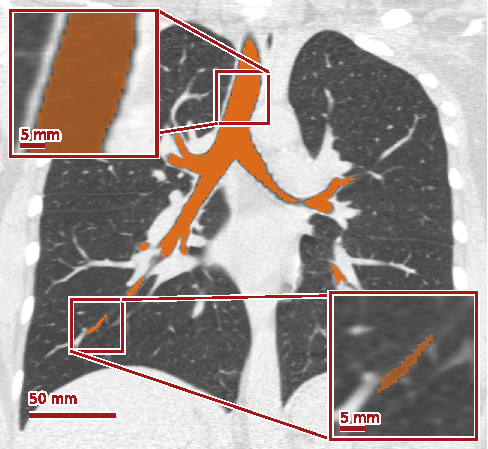
\includegraphics[width=\linewidth]{Figures/pdf/intro/airway_overview_slice.pdf}
    \caption{Coronal slice, reference airway overlaid. Both insets span
    \airwayInsetBox{}~mm; the magnified airways measure \airwayTracheaDiameter{}~mm
    and \airwayDistalDiameter{}~mm across.}
    % depth variant: Coronal slice, reference airway overlaid and split at branch
    % depth~\airwayProximalMaxGen{}. Both insets span \airwayInsetBox{}~mm; the
    % magnified airways measure \airwayTracheaDiameter{}~mm and
    % \airwayDistalDiameter{}~mm across.
    \label{fig:airway-overview-slice}
  \end{subfigure}\hfill
  \begin{subfigure}[b]{0.39\textwidth}
    \centering
    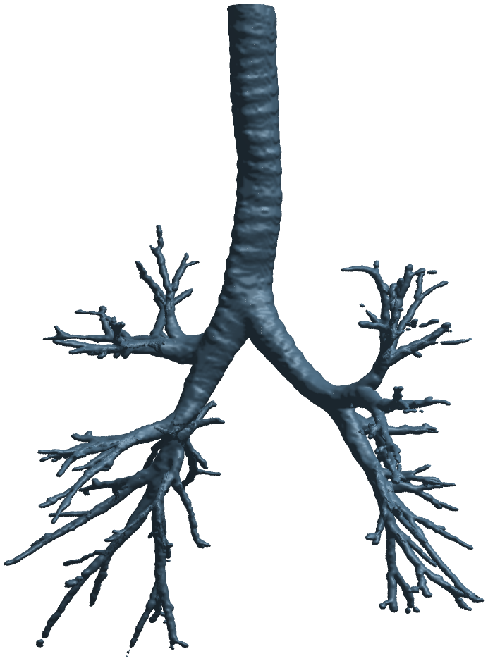
\includegraphics[width=\linewidth]{Figures/pdf/intro/airway_overview_tree_plain.pdf}
    \caption{The same tree in three dimensions.}
    % depth variant: The same tree, coloured by branch depth.
    \label{fig:airway-overview-tree}
  \end{subfigure}
  \caption[The airway tree in thoracic CT]{The airway tree in thoracic CT. ATM'22 case
  001~\cite{zhang2023atm22}, rendered for this study.}
  \label{fig:airway-overview}
\end{figure}

\section{Challenges in airway segmentation}
\label{sec:challenges}

Airway segmentation is difficult because two forms of imbalance occur simultaneously. The
first is the imbalance between airway foreground and background. Within the lung region supplied to the
network, annotated airway voxels form only a small fraction of the total volume
(Figure~\ref{fig:class-imbalance}). Moreover,
airway lumen and surrounding lung parenchyma can occupy overlapping intensity ranges, meaning
that the airway cannot be identified from voxel intensity alone. This becomes increasingly
important in peripheral branches, where the airway diameter approaches the spatial resolution
of the CT image and partial-volume effects reduce the distinction between lumen, airway wall
and surrounding tissue~\cite{montaudon2007,GarciaUceda2021AirwayCNN}.

A second imbalance exists within the airway foreground itself. The trachea and proximal
bronchi contain substantially more voxels than the numerous narrow distal branches. Consequently, the smallest
peripheral branches account for a small share of the segmented volume despite disproportionately determining the anatomical
extent of the reconstructed tree. A voxel-overlap objective such as Dice~\cite{dice1945association} is therefore dominated by the larger proximal structures
and can remain favourable even when a considerable proportion of the peripheral tree is absent~\cite{zhang2023atm22,zheng2021gradient}. 
This distinction is particularly important because airway segmentation is not simply a problem of recovering
foreground voxels, but of recovering a connected branching structure. A small discontinuity near a bifurcation may disconnect an
otherwise correctly segmented distal subtree while producing only a minor change in global
overlap.

% Placed after the two imbalance paragraphs because it evidences both: the rarity and
% intensity overlap of paragraph one, and the proximal/distal split of paragraph two.
% First referenced in paragraph one, so [tbp] can put it at the top of that page.
%
% The caption now defines generation depth and the proximal/distal split, so the
% panel legend is self-contained. What it deliberately does NOT carry is the
% justification for drawing the line there rather than at the clinical small-airway
% definition (under 2 mm, near generation eight), which sits below CT resolution and
% is largely absent from the annotation. That argument is prose, not caption; it is
% still only in the superseded section and should move up if it is wanted at all.
%
% The whole-scan version of this figure (denominator = uncropped volume, y-axis clipped above
% the parenchyma mode with the field-of-view air spike annotated) is still produced by
% dissertation/scripts/generate_hu_imbalance_histogram.py as
% Figures/pdf/background/airway_class_imbalance.pdf. It was cut deliberately: its extra
% content is the motivation for lung cropping, and its severity is partly produced by voxels
% preprocessing discards. Re-include it only if that motivation needs a figure of its own.
\begin{figure}[htbp]
  \centering
  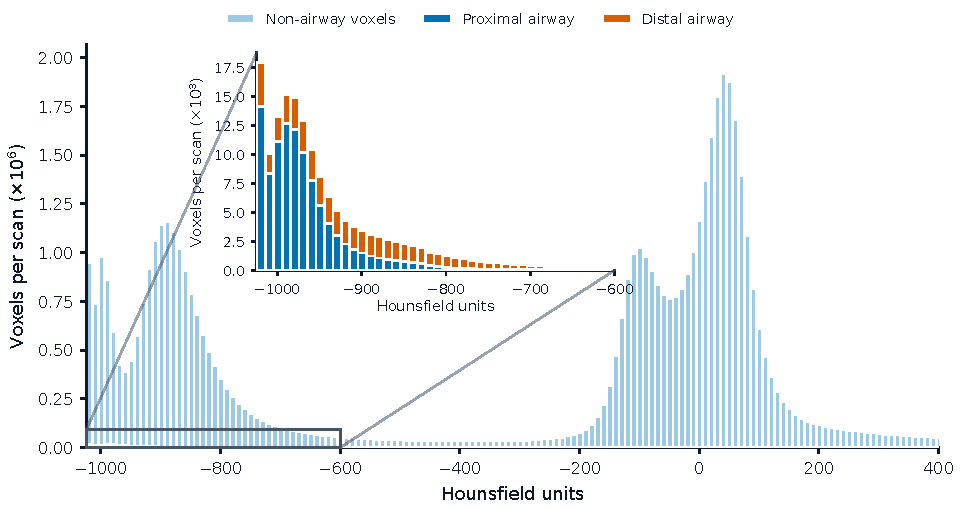
\includegraphics[width=\textwidth]{Figures/pdf/background/airway_class_imbalance_roi.pdf}
  \caption[Airway class imbalance by generation depth]{Hounsfield distribution of the lung
  region the network is trained on, over the \airwayNcases{} ATM'22 training scans. The airway
  window is magnified in both axes and split by generation depth: generation counts branch
  depth from the trachea (generation zero), so proximal is depth \airwayProximalMaxGen{} or
  less (trachea, main and lobar bronchi) and distal is everything beyond.}
  \label{fig:class-imbalance}
\end{figure}

Consequently, Dice overlap alone does not fully describe airway-tree quality. Airway benchmarks such as
ATM'22~\cite{zhang2023atm22} therefore complement volumetric overlap with measures such as tree-length-detection (TLD) and
branch-detection (BD). These measures emphasise recovery of the reference tree, 
but must themselves be interpreted alongside precision since overprediction may increase apparent tree coverage.

The same properties that make peripheral airways difficult to segment also make them difficult
to annotate. Dense three-dimensional airway masks are slow and expert-intensive to produce;
the reference annotations used by ATM'22 required approximately 60--90 minutes per scan~\cite{zhang2023atm22}. 
Annotation also becomes increasingly uncertain towards the distal tree,
where branches become narrow and poorly resolved. As a result, large collections of CT can be available
without their corresponding complete airway annotation. This motivates semi-supervised learning:
rather than requiring every training volume to carry a dense reference mask, unlabelled CT can potentially
provide an additional training signal by introducing wider anatomical variation.

\section{Prior work and unresolved gap}

Modern airway segmentation methods are predominantly based on encoder--decoder convolutional
networks derived from U-Net. In particular, nnU-Net provides a strong baseline because it
configures preprocessing, image spacing, patch size, network architecture, augmentation,
training schedule and inference around the properties of the dataset rather than treating the
network architecture in isolation~\cite{isensee2021nnunet}. This is important when evaluating additional
losses or training strategies: comparing different pipelines changes several factors
simultaneously, whereas a matched intervention within the same pipeline allows the effect of a
single component to be isolated.

Airway-specific methods have attempted to improve peripheral recovery through class weighting,
small-airway oversampling, skeleton-based hard-example mining and explicit reconnection of
broken branches~\cite{qin2019airwaynet,yu2022break,zhang2023atm22}. Results from ATM'22 suggest
that improvements in tree completeness arise from the complete training pipeline rather than
from a single loss function. The challenge results also illustrate an important limitation of
pure volumetric optimisation: methods with similar overlap can differ substantially in detected
tree length and branch recovery~\cite{zhang2023atm22}. This motivates incorporating geometry
directly when comparing airway predictions.

One such representation is clDice, which measures agreement using the centreline support of
two tubular masks~\cite{shit2021cldice}. Unlike volumetric Dice, its directional terms distinguish
between missing reference structure and additional predicted structure. It therefore provides
a natural geometry for measuring consistency between two airway predictions. However, clDice
does not itself guarantee anatomical correctness: the published topological result concerns
binary masks, whereas training requires finite differentiable skeletonisation of probability
maps. It is also relatively insensitive to airway calibre, and branches contribute according to
their length. For this reason, clDice is not
treated here as a replacement for conventional supervised objectives or evaluation metrics.
Instead, it is used as the geometry in which consistency between student and teacher
predictions is encouraged.

Semi-supervised segmentation methods attempt to exploit unlabelled images in addition to a
smaller labelled set. Pseudo-labelling assigns discrete labels to unlabelled examples before
using them as additional training targets. Mean Teacher instead maintains a second network
whose parameters are an exponential moving average of the student parameters and encourages
the student's prediction to remain consistent with the teacher under perturbation~\cite{tarvainen2017mean}. Importantly, the original Mean Teacher formulation supplies a
continuous teacher prediction rather than a thresholded pseudo-label.

Conventional Mean Teacher formulations enforce consistency voxel by voxel. Because background
voxels greatly outnumber airway voxels, accumulated background disagreement can dominate a
voxelwise objective even under patch-based training~\cite{zheng2021gradient}. The errors that matter clinically are also of the wrong kind for
such an objective: losing a narrow peripheral branch changes only a small number of foreground voxels
while removing a segment of the tree. This motivates asking whether consistency defined on
airway centreline geometry supplies a more useful unlabelled training signal than voxelwise
agreement alone, and that question is answered here by training both.

This distinction may matter particularly for airway segmentation. A label-starved teacher may
assign weak but non-zero probability to a peripheral branch that it does not recover at the
final inference threshold. Thresholding that prediction before computing consistency removes
this information entirely and makes the target behave more like online pseudo-labelling.
Conversely, retaining the continuous probability map preserves uncertainty, but does not
guarantee that the student will discover anatomy absent from the teacher. The central question
is therefore whether teacher-derived consistency can add peripheral structure or whether it
primarily consolidates the structures already represented by the teacher.

Existing semi-supervised work provides limited evidence for this question in sparse tubular
segmentation. An influential three-dimensional Mean Teacher application studied the
comparatively dense left atrium rather than a branching tree~\cite{yu2019uamt}.
Airway- and vessel-specific studies instead use feature specialisation, cross-geometry and
distance consistency, or pseudo-labelling to accommodate thin structures
~\cite{gu2023featurespecialisation,zhu2024crossgeometry,zhao2025vesselselftraining}. These studies
support the premise that voxel agreement alone may be insufficient, but their labelled fractions,
data and comparison pipelines differ. Semi-supervised models may also receive additional
optimisation, augmentation exposure or EMA inference relative to their supervised baselines.
Without a continuation control sharing that training envelope, an observed difference cannot be
assigned uniquely to the unlabelled consistency objective.

The unresolved gap addressed in this dissertation is therefore not simply whether a
semi-supervised model can obtain a higher headline Dice score. It is whether a
geometry-aware Mean Teacher can exploit unlabelled thoracic CT to recover airway-tree
structure beyond that learned from a limited labelled set, under the closest available matched
training comparison. A second question is whether any change is localised by airway calibre and
branch depth, and whether it is specific to centreline-aware rather than voxelwise agreement.

\section{Aim and objectives}

The aim of this dissertation is to determine whether geometry-aware Mean Teacher consistency
on unlabelled thoracic CT can improve airway-tree recovery under limited labelled supervision,
and to identify the mechanism by which any improvement or failure occurs.

To address this aim, the study:

\begin{enumerate}
    \item reports a label-limited supervised seed and a more fully labelled supervised model as
    scale references for the semi-supervised configurations;

    \item implements a two-stream Mean Teacher framework in which student predictions on
    unlabelled CT are regularised against an exponential-moving-average teacher using
    centreline-aware consistency;

    \item compares this model with a no-consistency continuation using the same training
    configuration;

    \ifshowcurrentcontrol
    \begin{currentcontrolroute}
    The available checkpoints estimate a configuration contrast but do not isolate consistency
    from independently realised output heads and training trajectories.
    \end{currentcontrolroute}
    \fi

    \ifshowpairedcontrol
    \begin{pairedcontrolroute}
    Prospective seed pairs additionally share the complete initial state and stochastic schedule,
    allowing variation in the fold-0 treatment effect to be estimated.
    \end{pairedcontrolroute}
    \fi

    \item tests consistency objective and weight as ablations, while
    separating changes in unlabelled pool size from changes in its training exposure;

    \item evaluates the resulting models using complementary volumetric and topology-aware
    measures, including Dice, detected tree length, branch detection and topology
    precision; and

    \item evaluates the final ordering on a held-out test cohort and on the external AeroPath
    dataset without dataset-specific tuning~\cite{stoverud2023aeropath}.
\end{enumerate}

The following chapter describes the datasets, nnU-Net training pipeline, Mean Teacher
implementation and matched experimental controls. The subsequent chapters report the
experimental results, interpret the observed behaviour and consider the implications and
limitations of geometry-aware semi-supervised learning for airway segmentation.

%\include{Chapters/Background}
% !TEX root = ../main.tex
% Chapter: Methods
\chapter{Methods}
\label{ch:methods}

% Booklet brief: detailed enough to reproduce.
%
% CUT PASS 2026-08-19 per methods_cut_guide.md. The chapter is now a definitional Methods,
% not a technical record: equations are protected, the prose around them is minimal.
%
% MOVED OUT of this chapter -- these are written and correct, they are just not Methods.
% Recover them from git history rather than rewriting:
%   -> APPENDIX A: region-of-interest audit (98-voxel superior overhang, margin sweep,
%      100% airway retention, ~75% volume discarded, per-case retention range); nnU-Net Dice
%      smoothing/aggregation convention; consistency instrumentation (gradient-norm probe,
%      teacher-evidence counters, same-patch counterfactual, objective decomposition);
%      checkpoint semantics (student vs final EMA teacher vs "best teacher" snapshot);
%      reproducibility audit (source hashes, launcher validation, cuDNN/GPU non-determinism,
%      the epoch-441 resume, prediction-metadata gap, test coverage).
%   -> DISCUSSION: clDice is not a zero-at-equality divergence for fractional maps, so part
%      of the term is irreducible binarisation pressure; the topology term is patch-local and
%      cannot enforce whole-lung connectivity; the failed class-balanced voxel-MSE arm; the
%      canonical-MT-vs-pseudo-labelling argument; the K/pool
%      compute confound; ATM'22 provenance (LIDC-IDRI + Shanghai Chest) for the ethics section.
%
% FIGURES DROPPED from Methods (files still exist, both are still built):
%   - fig:soft-skeleton-real-patch (4-panel real EMA-teacher patch) -- the operator schematic
%     covers the definition; this one illustrates, so it belongs in Results or Appendix A.
%
% STARRED / OPEN (2026-08-19) -- two things this chapter is waiting on:
%
%   1. A matched full-supervision reference on 260 labelled cases with
%      NoDeepSupervision + NoMirroring, single fold, no TTA. NOT RUN YET. The 110-label
%      reference currently in the chapter changes labels AND ensembling AND TTA at once, which
%      is why it is worded as a bracket rather than a ceiling. When the 260 arm exists, it
%      replaces that sentence and becomes the clean upper reference. See PROJECT_STATE.md.
%
%
% DO NOT re-add prose that defends a choice, interprets a result, or reports an audit.
% Every equation here was read off the implementation, not off a plan document.

\section{Study design and datasets}

All experiments were performed within a common nnU-Net pipeline, so that differences in
performance reflect the training strategy rather than the segmentation framework. ATM'22 was
used as the primary
dataset~\cite{zhang2023atm22,zhang2022cfda,zheng2021gradient,yu2022break,qin2019airwaynet,zhang2021fda}.
A fixed set of 20 cases was held out for external validation and a further 20 for final
testing; exact partitions are reported in Appendix~\ref{AppendixA}. AeroPath provided an
additional out-of-distribution test set of 27 thoracic CT volumes with airway
annotations~\cite{stoverud2023aeropath}, contributing airway anatomy altered by disease and CT
characteristics unlike those of ATM'22.

\section{Pre-processing and segmentation pipeline}
\label{sec:pipeline}

Volumes were left on their acquisition grid and affine. A lung and trachea region of interest
was constructed for every case from the CT and a lung mask inferred with the off-the-shelf
U-net(R231) model of \texttt{lungmask}~\cite{hofmanninger2020lungmask}, by expanding the
lung-mask bounding box by 8~voxels on its ordinary faces and by 120~voxels along the
affine-derived superior axis to retain the cervical trachea
(Figure~\ref{fig:lung-roi}). No annotation enters this construction, so the identical
field of view is available at inference.

All experiments used nnU-Net v2~\cite{isensee2021nnunet} in its three-dimensional
full-resolution configuration, under the settings of Table~\ref{tab:nnunet-config} derived by
the framework from the dataset fingerprint. Two defaults were disabled. Deep supervision was
disabled because the centreline objective of Section~\ref{sec:mean-teacher} erodes at a fixed
voxel scale and so has no consistent geometric meaning at downsampled auxiliary heads;
mirroring was disabled so that student and teacher views of a patch cannot differ by an
unmatched spatial transform. The resulting architecture is the PlainConvUNet of
Figure~\ref{fig:nnunet-backbone}, shared by student and teacher. Remaining pre-processing
detail, including the region-of-interest audit, is given in Appendix~\ref{AppendixA}.

\begin{figure}[htbp]
  \centering
  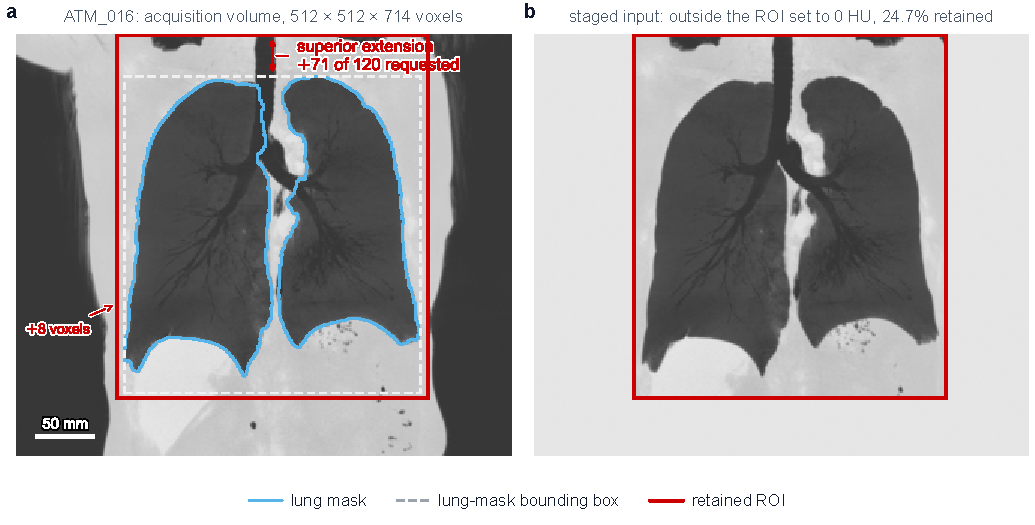
\includegraphics[width=\linewidth]{Figures/pdf/methods/lungroi/lung_roi_bbox.pdf}
  \caption[Airway region of interest]{The region of interest of Section~\ref{sec:pipeline} for
  ATM'22 case 016, coronal view. (a) Acquisition volume with the lung mask, its bounding box
  and the retained region. (b) The staged network input, with voxels outside the region set to
  $0$~HU; here $24.7\%$ of the volume is retained.}
  \label{fig:lung-roi}
\end{figure}

% ---------------------------------------------------------------------------
% ALTERNATIVE TO Figure~\ref{fig:lung-roi}, NOT AN ADDITION: the same staging drawn as a
% scene rather than as two coronal panels. Keep one, delete the other -- this block runs
% marker to marker. Drawn by dissertation/scripts/generate_lung_roi_3d_figure.py.
% ---------------------------------------------------------------------------
\begin{figure}[htbp]
  \centering
  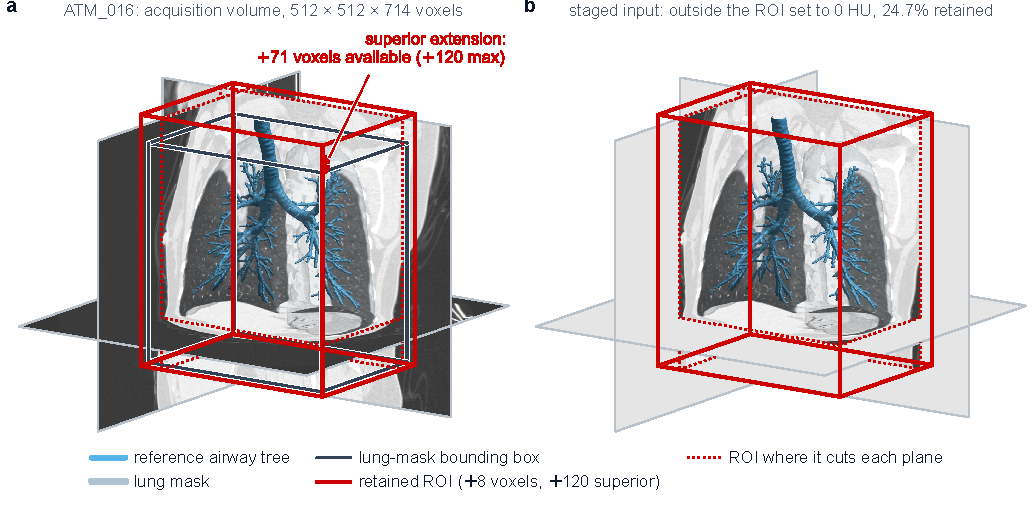
\includegraphics[width=\linewidth]{Figures/pdf/methods/lungroi/lung_roi_bbox_3d.pdf}
  \caption[Airway region of interest, three-dimensional]{The region of interest of
  Section~\ref{sec:pipeline} for ATM'22 case 016, seen from the patient's left and slightly
  above. Three orthogonal CT planes stand behind the anatomy, the lung mask is drawn as a
  translucent surface and the reference annotation as an isosurface; both boxes are drawn
  whole, in front of the scene, and dotted where the retained region cuts each plane. The
  solid box stands in front of the planes it is drawn over, so only the dotted rectangles
  meet the edge of the retained data. (a) Acquisition volume
  with the lung-mask bounding box and the retained region, whose superior face is raised to
  hold the cervical trachea; here the scan ends before the whole margin can be taken. (b)
  The staged network input, with voxels outside the region set to $0$~HU; here $24.7\%$ of
  the volume is retained. The airway tree is drawn for orientation only and takes no part
  in constructing the region, which is built from the lung mask alone. A coronal projection
  cannot show the anterior-posterior margin, which is two of the six faces.}
  \label{fig:lung-roi-3d}
\end{figure}
% ------------------------- end alternative figure --------------------------

\begin{table}[htbp]
  \centering
  \caption[nnU-Net configuration]{Planned and training configuration. Warm-started values apply
  to the Mean Teacher arms and the configuration-matched no-consistency continuation;
  supervised models use the from-scratch values.}
  \label{tab:nnunet-config}
  \begin{tabular}{ll}
    \toprule
    Setting & Value \\
    \midrule
    Configuration        & \texttt{3d\_fullres} \\
    Target spacing (mm)  & $0.820\times0.500\times0.820$ \\
    Patch size (voxels)  & $128\times160\times112$ \\
    Batch size           & 2 \\
    Normalisation        & \texttt{CTNormalization} (fingerprint percentiles) \\
    Optimiser            & SGD, Nesterov momentum 0.99, polynomial decay \\
    Learning rate        & $10^{-2}$ from scratch; $10^{-3}$ warm-started \\
    Schedule             & 1000 epochs from scratch; 500 warm-started, 250 iterations each \\
    Deep supervision     & disabled \\
    Mirroring            & disabled \\
    \bottomrule
  \end{tabular}
\end{table}

\begin{figure}[htbp]
  \centering
  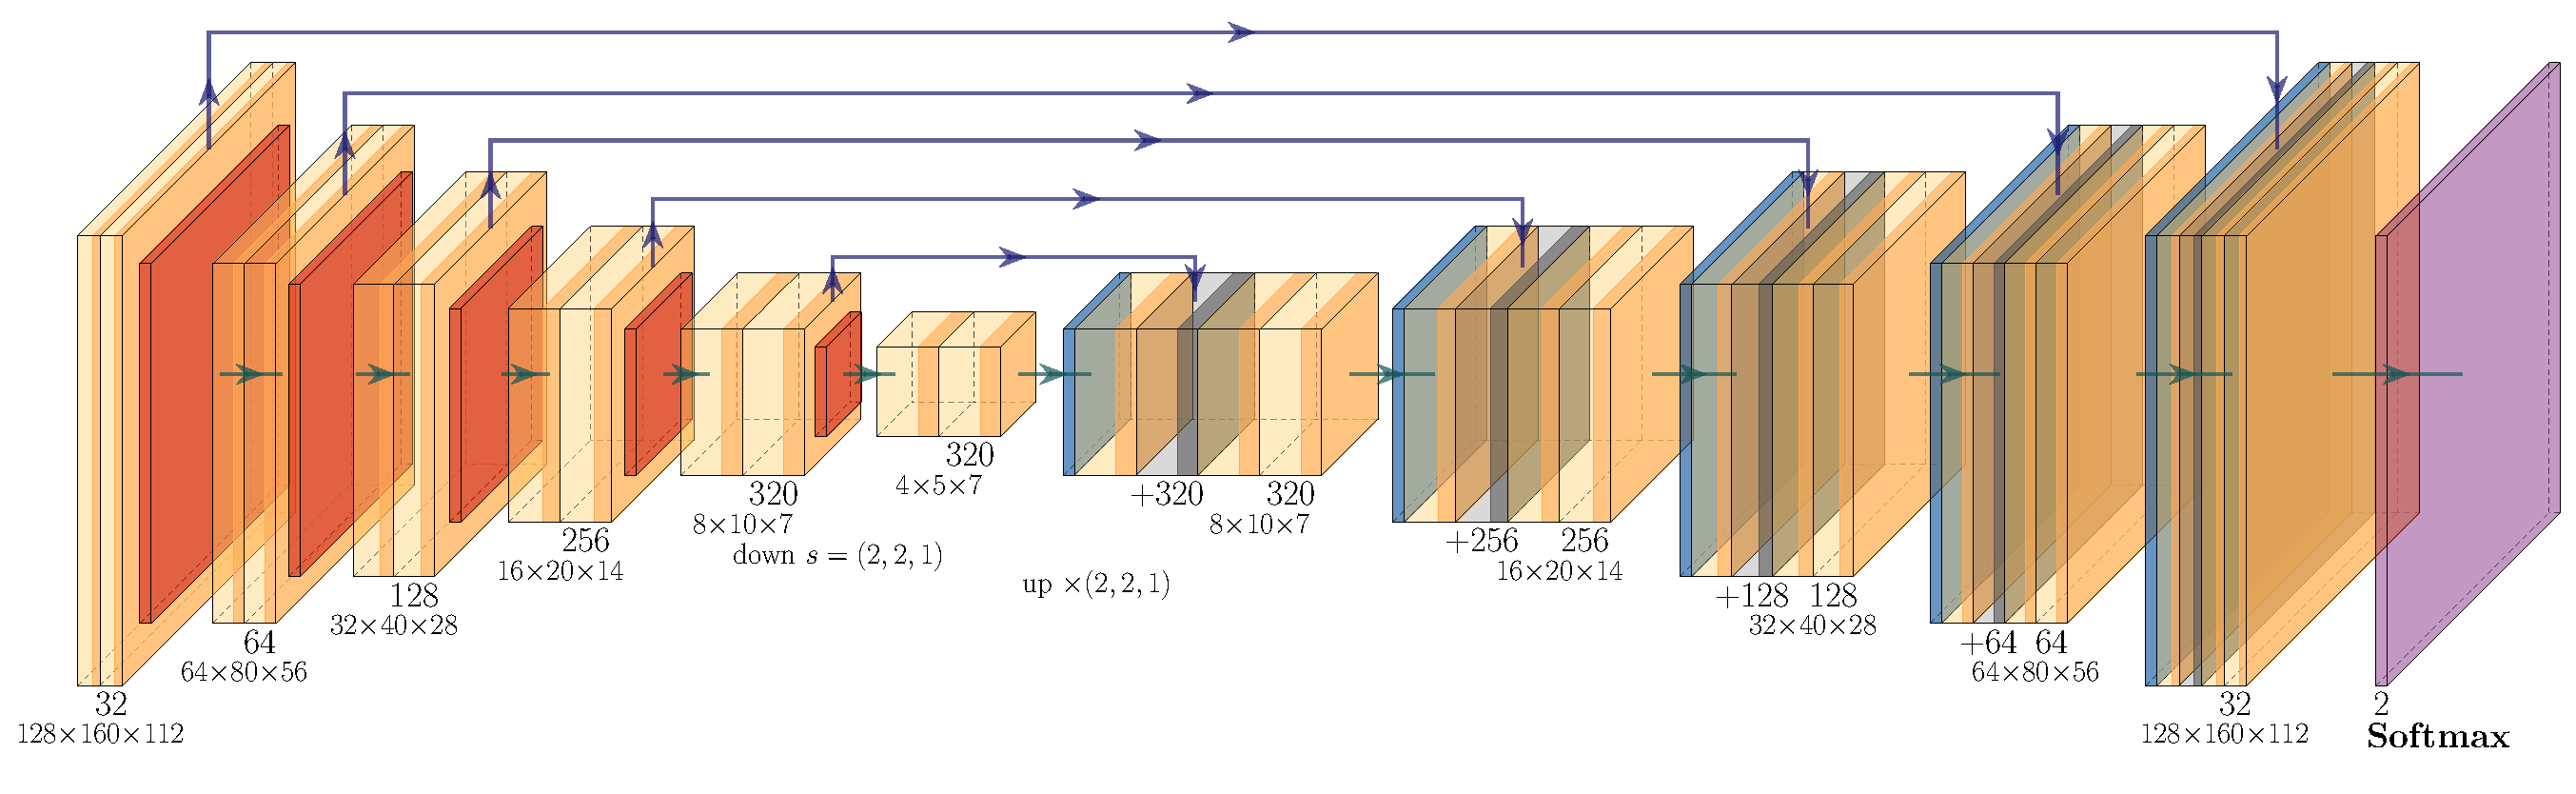
\includegraphics[width=\linewidth]{Figures/pdf/methods/mean_teacher/nnunet_backbone.pdf}
  \caption[Three-dimensional nnU-Net backbone]{The PlainConvUNet of
  Table~\ref{tab:nnunet-config}, shared by student and teacher. Block height and depth track
  spatial resolution and front-face width tracks channel count, with output channels and
  spatial size beneath each stage. Red slabs are strided convolutions, blue slabs transposed
  convolutions, and grey boxes the encoder features arriving on the skips. Drawn with
  PlotNeuralNet~\cite{iqbal2018plotneuralnet}.}
  \label{fig:nnunet-backbone}
\end{figure}

\section{Geometry-aware Mean Teacher}
\label{sec:mean-teacher}

\subsection{Notation and student--teacher formulation}

Let the labelled and unlabelled training sets be
\begin{equation}
  \mathcal{D}_{L}=\{(x_i,y_i)\}_{i=1}^{N_L},
  \qquad
  \mathcal{D}_{U}=\{x_j\}_{j=1}^{N_U},
  \label{eq:data}
\end{equation}
with $x$ a CT patch and $y\in\{0,1\}$ its airway annotation. Each step sampled one labelled and
one unlabelled patch. Writing $f_\theta$ for the airway probability channel of the softmax
output, the student with parameters $\theta_S$ and the teacher with parameters $\theta_T$ give
\begin{equation}
  p_{S,L}=f_{\theta_S}(\tilde{x}_L),
  \qquad
  p_{S,U}=f_{\theta_S}(\tilde{x}_U),
  \qquad
  p_{T,U}=f_{\theta_T}(x_U),
  \label{eq:predictions}
\end{equation}
where $\tilde{x}$ is the perturbed student view of Equation~\eqref{eq:perturbation}. The
teacher is not trained by back-propagation; its parameters are an exponential moving average of
the student's, updated after each optimiser step~\cite{tarvainen2017mean},
\begin{equation}
  \theta_T^{(t)}=\alpha_t\,\theta_T^{(t-1)}+(1-\alpha_t)\,\theta_S^{(t)},
  \qquad
  \alpha_t=\min\!\left(1-\frac{1}{t+1},\ \bar{\alpha}(e)\right),
  \label{eq:ema}
\end{equation}
with $t$ the step index and $e$ the epoch. Gradients flow only through the student, and the
final EMA teacher is the model used at inference. Figure~\ref{fig:mean-teacher-flow} shows the
resulting computation.

\begin{figure}[htbp]
  \centering
  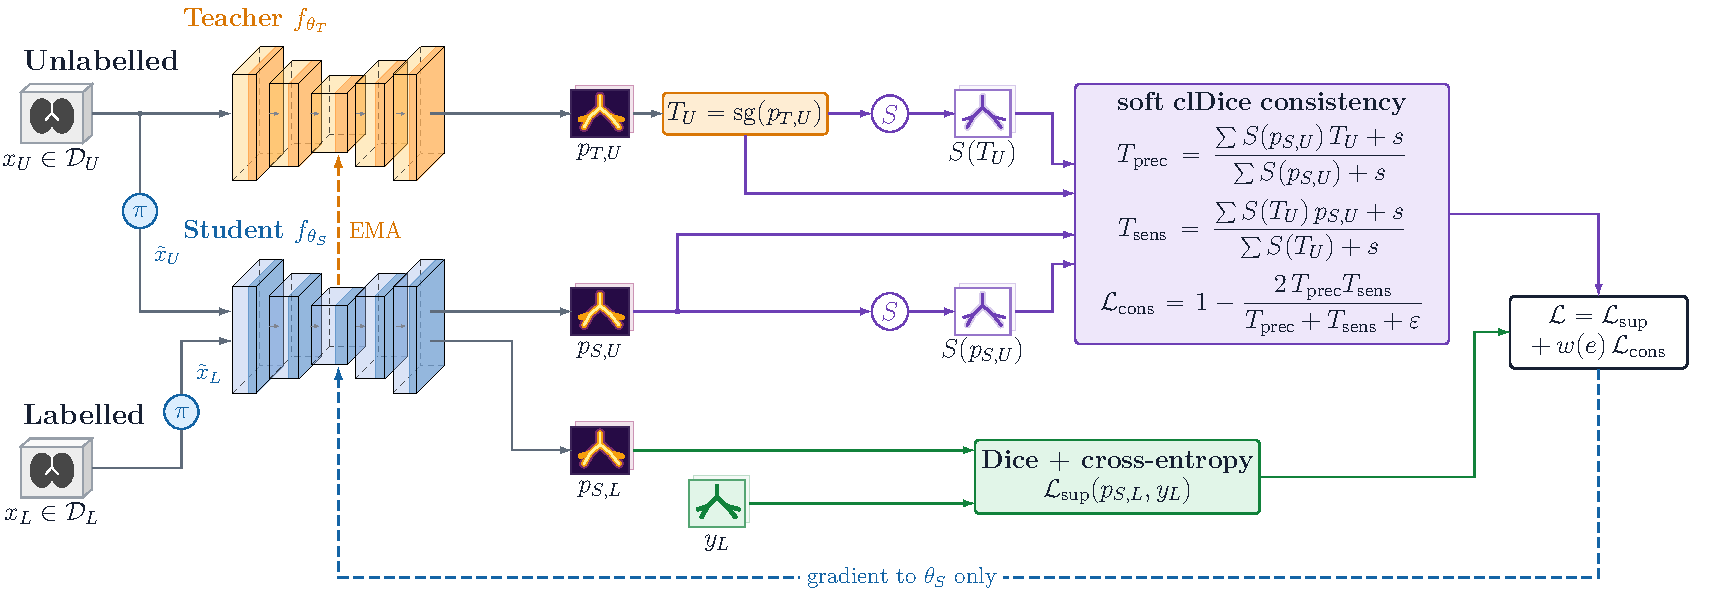
\includegraphics[width=\linewidth]{Figures/pdf/methods/mean_teacher/mean_teacher_flow.pdf}
  \caption[Two-stream Mean Teacher computation]{Two-stream Mean Teacher computation, with
  symbols as in Equations~\eqref{eq:data}--\eqref{eq:lcons}. Colour carries the roles: teacher
  warm, student blue, supervised path green and topology path purple, with back-propagation
  returning to the student alone along the dashed route. The image tiles are schematic rather
  than model outputs, and the network glyphs summarise the backbone of
  Figure~\ref{fig:nnunet-backbone}.}
  \label{fig:mean-teacher-flow}
\end{figure}

\subsection{Supervised objective}

The labelled stream uses nnU-Net's segmentation objective, the unweighted sum of soft Dice and
cross-entropy~\cite{isensee2021nnunet},
\begin{equation}
  \mathcal{L}_{\mathrm{sup}}(p,y)=\mathcal{L}_{\mathrm{Dice}}(p,y)+\mathcal{L}_{\mathrm{CE}}(p,y),
  \qquad
  \mathcal{L}_{\mathrm{Dice}}=1-\frac{2\sum_{\mathbf{u}}p(\mathbf{u})y(\mathbf{u})+\epsilon}
          {\sum_{\mathbf{u}}p(\mathbf{u})+\sum_{\mathbf{u}}y(\mathbf{u})+\epsilon},
  \label{eq:lsup}
\end{equation}
where $\mathbf{u}$ indexes voxels and $\epsilon$ is the framework's smoothing constant.

\subsection{Student perturbation}

The teacher receives the base view of an unlabelled patch and the student an additional
intensity perturbation,
\begin{equation}
  \tilde{x}=\pi(x)=a\,x+b+\eta,
  \qquad
  a\sim\mathcal{U}(1-s_a,\,1+s_a),
  \quad
  b\sim\mathcal{U}(-s_b,\,s_b),
  \quad
  \eta\sim\mathcal{N}(0,\sigma^2),
  \label{eq:perturbation}
\end{equation}
with $s_a=s_b=\sigma=0.1$, applied from epoch 5 to the student's whole input. Ordinary nnU-Net
augmentation is applied upstream and is therefore shared by both views, so the two outputs are
voxel-aligned and no inverse transform is required.

\subsection{Differentiable centreline extraction}

The consistency term compares centrelines, which requires a differentiable skeletonisation. The
implementation follows Shit et al.~\cite{shit2021cldice}, whose operators are the grey-scale
erosion and dilation of mathematical morphology under flat structuring
elements~\cite{serra1982morphology,haralick1987morphology,soille2003morphology}. Soft erosion
takes the minimum over a voxel and its six face-connected neighbours and soft dilation takes the
maximum over the full $3\times3\times3$ neighbourhood,
\begin{equation}
  \mathcal{E}(X)(\mathbf{u})=\!\!\min_{\mathbf{v}\in\mathcal{N}_6(\mathbf{u})\cup\{\mathbf{u}\}}\!\!X(\mathbf{v}),
  \qquad
  \mathcal{D}(X)(\mathbf{u})=\!\!\max_{\mathbf{v}\in\mathcal{N}_{26}(\mathbf{u})\cup\{\mathbf{u}\}}\!\!X(\mathbf{v}),
  \label{eq:morph}
\end{equation}
where $X$ is the input probability map, $\mathbf{u}$ denotes the voxel at which the operator
is evaluated, and $\mathbf{v}$ indexes voxels in its neighbourhood. 
$\mathcal{N}_6(\mathbf{u})$ and $\mathcal{N}_{26}(\mathbf{u})$ denote respectively the six
face-connected and the 26 surrounding neighbours of voxel $\mathbf{u}$.
Their composition $\mathcal{O}=\mathcal{D}\circ\mathcal{E}$ is the soft opening
of Shit et al.~\cite{shit2021cldice}. Ridge evidence at erosion depth $k$ is the positive part of what
the soft opening removes, an opening residual analogous to a white
top-hat~\cite{soille2003morphology}, and successive depths are combined by a differentiable
union,
\begin{align}
  X^{(0)}&=X,
  \qquad
  X^{(k)}=\mathcal{E}\!\left(X^{(k-1)}\right),
  \quad k=1,\dots,K,
  \nonumber\\
  \delta^{(k)}&=\operatorname{ReLU}\!\left(X^{(k)}-\mathcal{O}\!\left(X^{(k)}\right)\right),
  \quad k=0,\dots,K,
  \label{eq:residual}\\
  S^{(0)}&=\delta^{(0)},
  \qquad
  S^{(k)}=S^{(k-1)}+\operatorname{ReLU}\!\left(\delta^{(k)}-S^{(k-1)}\delta^{(k)}\right),
  \quad k=1,\dots,K.
  \label{eq:accumulate}
\end{align}
Residuals are therefore taken at depth $0$ and after each of $K=10$ erosion updates, and we
write $S(\cdot)=S^{(K)}$ for the resulting soft skeleton, illustrated in
Figure~\ref{fig:soft-skeleton-iteration} and set out procedurally in
Algorithm~\ref{alg:soft-skeleton}. Equations~\eqref{eq:residual} and~\eqref{eq:accumulate}
follow the form of Lantu\'ejoul's skeleton by
openings~\cite{lantuejoul1980skeleton,serra1982morphology}, with the set union over erosion
depths replaced by the probabilistic sum $a+b-ab$, the standard fractional union that keeps the
accumulation differentiable~\cite{klir1995fuzzy,bloch1995fuzzymorphology}.

\begin{figure}[htbp]
  \centering
  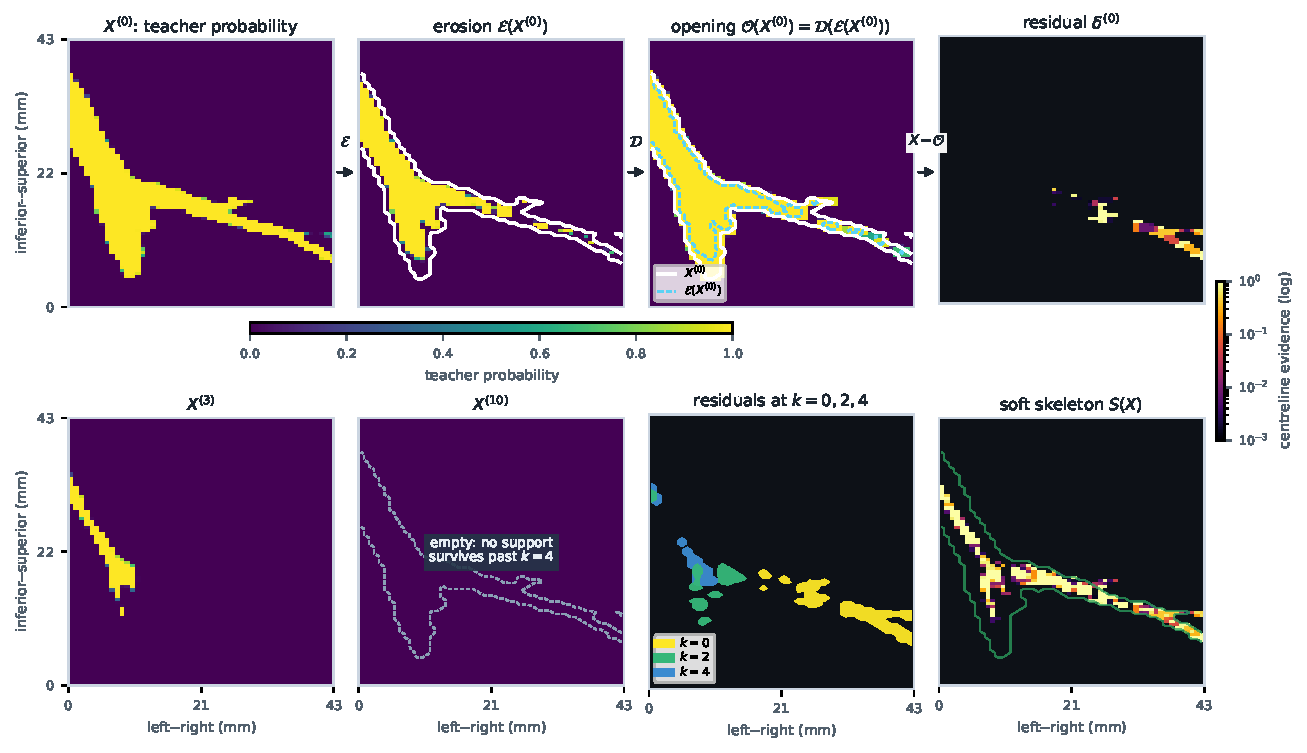
\includegraphics[width=\linewidth]{Figures/pdf/methods/cldice/soft_skeleton_iteration.pdf}
  \caption[Differentiable soft skeletonisation]{Equations~\eqref{eq:morph}--\eqref{eq:accumulate}
  on a real EMA-teacher airway-probability patch, as a maximum projection through a seven-voxel
  coronal slab. Top row, one iteration: erosion, the opening $\mathcal{O}(X^{(0)})$, and the
  residual $\delta^{(0)}$. Contours give $X^{(0)}$ at $0.5$ (solid white) and where erosion left
  it (dashed cyan), so the trunk is regrown by the dilation and the thin distal branch is not.
  Bottom row, successive erosion depths and their union, the soft skeleton $S(X)$; the grey
  dashed outline marks the original airway support. Green is the reference airway, for
  orientation only.}
  \label{fig:soft-skeleton-iteration}
\end{figure}

An implementation-matched diagnostic quantified how this finite operator allocated its mass.
Six foreground-centred, training-shaped patches were sampled from each of four final EMA-teacher
probability maps. Teacher foreground and $S(T_U)$ were assigned to the operational calibre of the
nearest reference centreline voxel, and their mass shares were aggregated over the 24 patches.
The calculation was repeated after twofold trilinear upsampling, using $K=20$ to preserve the
physical erosion range, and timed with gradient checkpointing. This probe characterises the
implemented loss on fitted predictions; it is not a training arm or an estimate of the Mean
Teacher effect.

\subsection{Geometry-aware consistency}
\label{sec:consistency}

The consistency target is the detached teacher probability map,
$T_U=\operatorname{sg}(p_{T,U})$, where $\operatorname{sg}$ denotes the stop-gradient. Student
and target are compared by the topology precision and topology sensitivity of Shit et
al.~\cite{shit2021cldice},
\begin{equation}
  T_{\mathrm{prec}}
  =\frac{\sum_{\mathbf{u}}S(p_{S,U})T_U+s}{\sum_{\mathbf{u}}S(p_{S,U})+s},
  \qquad
  T_{\mathrm{sens}}
  =\frac{\sum_{\mathbf{u}}S(T_U)\,p_{S,U}+s}{\sum_{\mathbf{u}}S(T_U)+s},
  \label{eq:tterms}
\end{equation}
with smoothing $s=1$ in numerator and denominator, and the consistency loss is one minus their
harmonic mean,
\begin{equation}
  \mathcal{L}_{\mathrm{cons}}
  =1-\frac{2\,T_{\mathrm{prec}}T_{\mathrm{sens}}}{T_{\mathrm{prec}}+T_{\mathrm{sens}}},
  \label{eq:lcons}
\end{equation}
which is soft clDice~\cite{shit2021cldice}, here evaluated between the student and the EMA
teacher rather than between a prediction and an annotation. Both terms are computed per sample
and averaged over the batch.

The voxel-MSE arm replaces Equation~\eqref{eq:lcons} with the squared-error consistency of
Tarvainen and Valpola~\cite{tarvainen2017mean}, applied per voxel to the airway channel as in
semi-supervised 3D segmentation~\cite{yu2019uamt},
\begin{equation}
  \mathcal{L}_{\mathrm{MSE}}
  =\frac{1}{|\Omega|}\sum_{\mathbf{u}\in\Omega}
   \left(p_{S,U}(\mathbf{u})-T_U(\mathbf{u})\right)^{2},
  \label{eq:lmse}
\end{equation}
over the patch domain $\Omega$, with every other setting held fixed.

Wallace and Dahabreh define separate class-specific Brier scores~\cite{wallace2014imbalanced};
Bellinger et al. average these to form the balanced Brier score~\cite{bellinger2020remix}.
Adapting this to soft teacher targets, voxels were split into teacher-predicted foreground
($\geq0.5$) and background ($<0.5$). For non-empty groups,
\begin{equation}
  \begin{aligned}
    \mathrm{MSE}_{\mathrm{fg}}
    &=\frac{1}{N_{\mathrm{fg}}}
      \sum_{\substack{\mathbf{u}\in\Omega\\T_U(\mathbf{u})\geq0.5}}
      \left(p_{S,U}(\mathbf{u})-T_U(\mathbf{u})\right)^2,\\
    \mathrm{MSE}_{\mathrm{bg}}
    &=\frac{1}{N_{\mathrm{bg}}}
      \sum_{\substack{\mathbf{u}\in\Omega\\T_U(\mathbf{u})<0.5}}
      \left(p_{S,U}(\mathbf{u})-T_U(\mathbf{u})\right)^2,\\
    \mathcal{L}_{\mathrm{balMSE}}
    &=\frac{1}{2}\left(\mathrm{MSE}_{\mathrm{fg}}+\mathrm{MSE}_{\mathrm{bg}}\right),
  \end{aligned}
  \label{eq:lbalancedmse}
\end{equation}
where $N_{\mathrm{fg}}$ and $N_{\mathrm{bg}}$ are the respective voxel counts; an empty
group contributed zero. This gives each predicted group equal weight without centreline geometry.

\subsection{Training objective and schedule}

The total objective is the supervised loss plus a ramped consistency term,
\begin{equation}
  \mathcal{L}=\mathcal{L}_{\mathrm{sup}}\!\left(p_{S,L},y_L\right)
  +w(e)\,\mathcal{L}_{\mathrm{cons}}\!\left(p_{S,U},T_U\right),
  \label{eq:total}
\end{equation}
with the Gaussian ramp of Laine and Aila~\cite{laine2017temporal},
\begin{equation}
  w(e)=w_{\max}\exp\!\left[-5\left(1-r(e)\right)^{2}\right],
  \qquad
  r(e)=\operatorname{clamp}\!\left(\frac{e-e_0}{e_r},\,0,\,1\right),
  \label{eq:ramp}
\end{equation}
and $w(e)=0$ for $e<e_0$. Following UA-MT~\cite{yu2019uamt} we set $w_{\max}=0.1$, with warm-up
$e_0=5$ epochs and ramp $e_r=20$ epochs. The EMA ceiling $\bar{\alpha}$ of
Equation~\eqref{eq:ema} is $0.99$ during the ramp and $0.999$
afterwards~\cite{tarvainen2017mean}. Warm-started training ran for 500 epochs at initial
learning rate $10^{-3}$, following nnU-Net's fine-tuning
guidance~\cite{nnunetdocs_finetuning,wald2024maepretraining}; each Mean Teacher fold was
warm-started from its same-numbered supervised checkpoint.

\section{Experimental design}
\label{sec:experimental-design}

Continuation arms used 16 labelled training cases, four internal-validation cases and 240
label-withheld cases, with a common crop, architecture, sampler, schedule and final EMA
deployment. The primary contrast was
\begin{equation}
  \mathcal{L}_{\mathrm{control}}=\mathcal{L}_{\mathrm{sup}},
  \qquad
  \mathcal{L}_{\mathrm{MT}}=\mathcal{L}_{\mathrm{sup}}+w(e)\,\mathcal{L}_{\mathrm{cons}}.
  \label{eq:contrast}
\end{equation}
The control omitted the unlabelled gradient and teacher forward pass.

\ifshowcurrentcontrol
\begin{currentcontrolroute}
\noindent\textbf{Current fitted-checkpoint route.}
The scored control and Mean Teacher runs named the same supervised warm start, but transfer
excluded their segmentation heads and their RNG, augmentation and CUDA trajectories were
independent. They therefore provide a single-run configuration contrast, not a realised-paired
control.
\end{currentcontrolroute}
\fi

\ifshowpairedcontrol
\begin{pairedcontrolroute}
\noindent\textbf{Prospective paired-seed route.}
Five fold~0 control--Mean Teacher pairs load the same complete checkpoint within each pair and
share the seeded data order, augmentation draws and deterministic CUDA settings. Only pairs in
which both arms finish are analysed; three complete pairs are the minimum.
\end{pairedcontrolroute}
\fi

Plain and class-balanced voxel MSE, consistency weight and skeleton depth are ablations; the
five-fold Mean Teacher ensemble and 110-case supervised model provide deployment and scale
context, respectively.

\begin{table}[htbp]
  \centering
  \small
  \setlength{\tabcolsep}{3pt}
  \caption[Experimental arms and their scientific roles]{Experimental arms retained in the
  main study. ``L'' and ``U'' denote labelled and label-withheld training cases.}
  \label{tab:experimental-arms}
  \begin{tabular}{@{}>{\raggedright\arraybackslash}p{0.16\linewidth}
                      >{\raggedright\arraybackslash}p{0.25\linewidth}
                      >{\raggedright\arraybackslash}p{0.13\linewidth}
                      >{\raggedright\arraybackslash}p{0.36\linewidth}@{}}
    \toprule
    Role & Arm & Training data & Question answered \\
    \midrule
    \ifshowcurrentcontrol
    \textcolor{ImperialBlue}{Current contrast} & \textcolor{ImperialBlue}{Control and soft-clDice MT} & \textcolor{ImperialBlue}{16 L $+$ 240 U} & \textcolor{ImperialBlue}{Available fitted-checkpoint comparison} \\
    \fi
    \ifshowpairedcontrol
    \textcolor{ImpRed}{Seeded contrast} & \textcolor{ImpRed}{Five control--soft-clDice pairs} & \textcolor{ImpRed}{16 L $+$ 240 U} & \textcolor{ImpRed}{Training-run variation at fixed fold} \\
    \fi
    Objectives & Plain and balanced voxel MSE & 16 L $+$ 240 U & Geometry versus voxel agreement \\
    Parameters & Soft-clDice weight and skeleton depth & 16 L $+$ 240 U & Sensitivity around the primary setting \\
    Deployment & Five-fold soft-clDice ensemble & 16 L/fold $+$ 240 U & Absolute ensemble performance \\
    References & 16-label seed; 110-case supervised model & 16 L; 88 L & Warm-start and label-scale context \\
    \bottomrule
  \end{tabular}
\end{table}

\section{Inference and post-processing}

Predictions used nnU-Net's sliding-window inference without test-time augmentation, and the
native argmax output is the primary result; no probability threshold was tuned. For Mean
Teacher arms the final EMA teacher is the model evaluated. A single connected-component
sensitivity analysis is reported alongside, retaining the six-connected component that
intersects an affine-derived window covering the superior quarter and the central half of each
remaining axis, and falling back to the largest component if none intersects. Checkpoint
provenance is given in Appendix~\ref{AppendixA}.

\section{Evaluation protocol and tree analysis}
\label{sec:evaluation}

\subsection{Voxel-level and topology-aware metrics}

Let $P$ be the predicted foreground and $G$ the reference airway mask, with
\begin{equation}
  \operatorname{Dice}=\frac{2|P\cap G|}{|P|+|G|},
  \qquad
  \operatorname{Prec}=\frac{|P\cap G|}{|P|},
  \qquad
  \operatorname{Rec}=\frac{|P\cap G|}{|G|}.
  \label{eq:voxel}
\end{equation}
Following the ATM'22 protocol the reference is reduced to its largest connected component
before skeletonisation, which uses three-dimensional medial-axis thinning~\cite{lee1994thinning}. Writing $S_G$ for that skeleton and $S_P$ for the skeleton of the
prediction, tree-length detected and topology precision are
\begin{equation}
  \operatorname{TLD}=\frac{|S_G\cap P|}{|S_G|},
  \qquad
  \operatorname{TPrec}=\frac{|S_P\cap G|}{|S_P|}.
  \label{eq:tld}
\end{equation}
Branch detection parses $S_G$ into branches by removing junction
voxels and discarding fragments shorter than five voxels; for reference branch $b$ with
skeleton $S_b$,
\begin{equation}
  c_b=\frac{|S_b\cap P|}{|S_b|},
  \qquad
  \operatorname{BD}=\frac{1}{N_B}\sum_{b=1}^{N_B}\mathbf{1}\!\left[c_b\ge0.8\right].
  \label{eq:bd}
\end{equation}
Dice, voxel precision, TLD and BD are the four primary measures. Where reported, the secondary
ATM-style clDice quantity is the harmonic mean
$2\,\operatorname{TLD}\operatorname{TPrec}/
(\operatorname{TLD}+\operatorname{TPrec})$. Because its TLD term uses the largest connected
component of the reference while its topology-precision term uses the full prediction, this is
a mixed-support diagnostic rather than standard full-mask clDice. All metrics are computed per
patient and reported as macro means over cases.

\subsection{Calibre-stratified recovery}
\label{sec:methods-calibre}

Recovery was stratified by local airway calibre, defined granulometrically as what a voxel fits
inside~\cite{matheron1975randomsets,serra1982morphology}. The operational calibre uses the
operators of Equation~\eqref{eq:morph}, so that it speaks about what the training objective can
resolve,
\begin{equation}
  n(\mathbf{u})=\max\left\{n:\ \mathbf{u}\in\mathcal{D}^{\,n}\!\left(\mathcal{E}^{\,n}(G)\right)\right\},
  \label{eq:opclass}
\end{equation}
where class $n$ corresponds to a thickness of $\{2n+1,2n+2\}$ voxels, so that the histogram of
$n$ over the reference tree is an opening size distribution, or pattern
spectrum~\cite{maragos1989patternspectrum,soille2003morphology}.
Intuitively, $n(\mathbf{u})$ is the largest erosion--dilation scale that the airway
surrounding $\mathbf{u}$ survives; larger values therefore correspond to locally thicker
airways.

The anatomical calibre is the Euclidean local thickness in millimetres, the diameter of the
largest ball that fits inside the structure and contains the
voxel~\cite{hildebrand1997thickness,dougherty2007localthickness},
\begin{equation}
  \tau(\mathbf{u})=2\max\left\{r:\ \mathbf{u}\in\mathcal{O}_{r}(G)\right\},
  \label{eq:mmthickness}
\end{equation}
with $\mathcal{O}_r$ opening by a ball of radius $r$ on the voxel spacing. Both refer to lumen
calibre, not airway-wall thickness.

Writing $S_G^{(k)}$ for the reference centreline voxels in
band $B_k$ under either definition, band-wise recovery is
\begin{equation}
  \operatorname{TLD}_k=\frac{\left|S_G^{(k)}\cap P\right|}{\left|S_G^{(k)}\right|}.
  \label{eq:tldband}
\end{equation}
Calibre is defined from the reference tree and the same banding is applied to every arm.

\subsection{Branch-depth analysis}
\label{sec:methods-depth}

Branch depth was used as a measure of position within the airway tree, following the
established practice of reducing a segmented tree to its centreline and analysing it branch by
branch~\cite{tschirren2005airway,palagyi2006airway}. The reference
skeleton was first divided into branches as in Equation~\eqref{eq:bd}, and these branches
were connected to form a graph. The ATM'22 branch-refinement procedure was then applied
iteratively until the graph no longer changed. In particular, consecutive branch fragments
connected through only a single child were absorbed into the same path, so that depth
increased at branch divisions rather than at every skeleton fragment.

On the resulting branch graph $G_B=(V_B,E_B)$, each node $v\in V_B$ represents a refined
airway branch and each edge represents a connection between branches. The largest-volume
branch was taken as the graph root; in practice this corresponded to the tracheal branch
in the reference trees examined,
\begin{equation}
  v_0=\operatorname*{arg\,max}_{v\in V_B}\operatorname{Vol}(v),
\end{equation}
and the depth of branch $v$ was defined as its graph distance from this root,
\begin{equation}
  d(v)=\operatorname{dist}_{G_B}(v_0,v).
  \label{eq:depth}
\end{equation}

Thus, $d(v)$ approximately counts the number of successive branch divisions separating a
branch from the trachea. It is therefore treated as a branching-order proxy
rather than as an anatomical Weibel generation~\cite{weibel1963morphometry}, which is fixed by
anatomical correspondence rather than by distance on a parsed
graph~\cite{tschirren2005airway}.

Figure~\ref{fig:branch-depth-definition} shows this assignment on an example reference tree
together with the distribution of annotated centreline length over depth across all 260
training cases. Reference centreline length is concentrated around intermediate depths,
peaking at depth six, and the external validation cohort follows the same distribution to
within 2.3 percentage points at every depth. Airway trees do not all end at the same
generation: the shallowest validation tree ends at depth eight, and only 46 of the 260 training
cases reach depth twelve. Depth-stratified recovery is therefore reported over depths zero to
seven individually, with depths eight and above pooled as $8+$, which keeps all 20 cases in
every point and retains the deep tree rather than discarding it.

\begin{figure}[htbp]
  \centering
  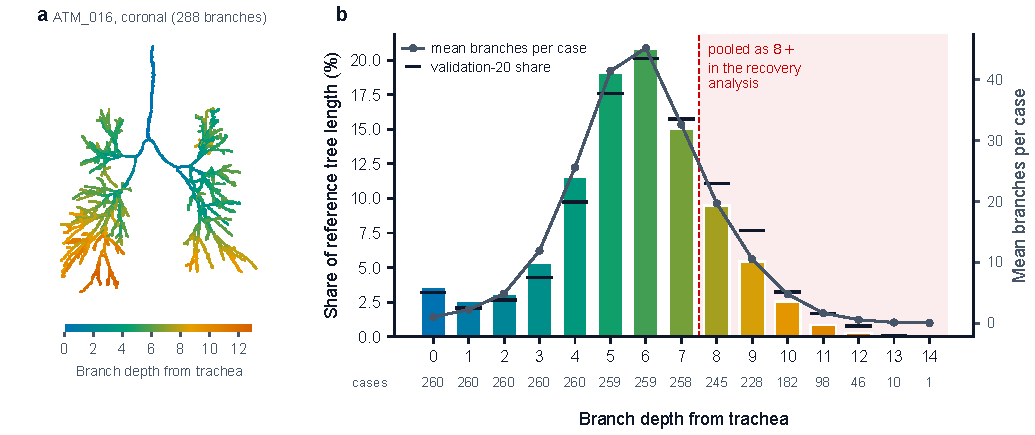
\includegraphics[width=\linewidth]{Figures/pdf/methods/depth/branch_depth_definition.pdf}
  \caption[Branch-depth coordinate and cohort distribution]{The branch-depth coordinate of
  Equation~\eqref{eq:depth}. (a) Coronal projection of the ATM\_016 reference skeleton, each
  centreline voxel coloured by the depth of its refined branch; the patient's right is on the
  left. (b) Share of annotated centreline length at each depth over the 260 training cases
  (bars, left axis), mean refined branches per case (line, right axis), and the corresponding
  share in the 20-case external validation cohort (black dashes). The row beneath the axis
  gives how many cases reach each depth. Shading marks the depths pooled into the $8+$ bin of
  the depth-stratified results.}
  \label{fig:branch-depth-definition}
\end{figure}

For a depth group $D_k$, the corresponding reference centreline is
\begin{equation}
  S_G^{(k)}
  =
  \bigcup_{v:\,d(v)\in D_k} S_v,
\end{equation}
and recovery within that group is calculated using the band-wise TLD definition of
Equation~\eqref{eq:tldband}. Depth labels are derived only from the reference tree and are
applied identically to every model.

\paragraph{Statistical comparisons.}
The patient is the unit of evaluation and checkpoint comparisons are paired because every arm
segments the same cases. Per-patient arm-minus-comparator differences are summarised by their
mean, the number favouring the arm, a pointwise 95\% paired-$t$ interval and the standardised
effect $d_z$; figures explicitly labelled as bootstrap intervals instead resample patients as
pairs. Two-sided paired $t$-tests are accompanied by Wilcoxon signed-rank tests, with
Bonferroni correction within each contrast across Dice, voxel precision, TLD, BD and the
secondary ATM-style clDice diagnostic. These patient-level intervals condition on the fitted
checkpoints and do not estimate training-run variation. For the prospective replication, a
cohort-mean treatment effect is first calculated within each complete seed pair and the
resulting replicate-level effects are reported by their mean, standard deviation and range;
patients from different training replicates are not treated as independent observations.

\section{Reproducibility}

Exact case identifiers, per-arm memberships, fold assignments, configuration files, training
commands and checkpoint provenance are provided in Appendix~\ref{AppendixA}. Training used
non-deterministic CUDA operations and mixed precision, and each experimental configuration was
trained once, so results are reproducible as a configuration rather than bitwise.

% !TEX root = ../main.tex
% Chapter: Results
\chapter{Results}
\label{ch:results}

% Booklet brief: "punchy and dry" -- present results, NO interpretation (that belongs in the
% Discussion). Curate hard: <=20 figures + tables TOTAL across the whole report.
%
% REWIRED 2026-08-14. Ordering principle: the chapter runs PRIMARY -> ABLATION -> CONTEXT,
% not chronologically. The soft-clDice arm and its exact control are the primary result and
% are still training, so they appear as marked placeholders at the TOP, not appended at the
% end. Everything from the from-scratch MONAI era (sealed-test three-model table,
% 128-cubed patches, reduced downsampling, distal sampling, calibre weighting, gap
% reconnection) has been REMOVED to Appendix A.
%
% NAMING: use descriptive arm names in prose (labelled-only seed, MT90, MT240, exposure arm),
% not internal dataset numbers. Internal IDs are kept in comments for traceability only.
% This is a COMPLIANCE point, not a style preference: the Guide states the assessors (at
% least two academic staff besides the module lead) will not have followed the project, so
% unexplained internal shorthand costs marks for clarity.
%
% FIGURE/TABLE BUDGET: 20 combined across the whole body, appendix excluded. Six figures are
% already committed (2 Background/Methods clDice+skeleton, backbone, MT flow, target
% construction, target skeletons). Every FIGURE/TABLE CANDIDATE below must therefore earn
% its slot. The grade rubric rewards figures that "incorporate relevant and ORIGINALLY
% PRESENTED content" -- the paired per-case delta plot and the diagnostics dashboard are the
% two most original artefacts available here, so protect those slots first.
%
% EXCLUDED BY DESIGN -- do not reinstate: the cold-start MT arm whose uniform sampler produced
% warm-up batches with no supervised gradient. That is an implementation fault, not a
% scientific result. It is named once in Methods/Discussion as a protocol lesson and nowhere
% else. Same for the loss-ablation arm that was walltime-truncated at epoch 319/1000 -- if it
% appears at all, it is labelled an early-checkpoint snapshot, never a completed ablation.
%
% ROUGH DRAFT: descriptive only. All "why" statements belong in Chapter 5.
% FORMAT: introduce each display, state only a non-obvious pattern, and never transcribe rows
% of values into prose. The displays carry the numerical record; interpretation belongs in
% Discussion and supporting breakdowns in Appendix A.

% OUTSTANDING RESULTS (2026-08-19). Every item below has a \pending marker in the
% text or a \pending row in a table, so grep for "\pending" to find them all. The
% document must contain none at submission.
%
%   1. Soft-clDice five-fold -- COMPLETE and entered in tab:primary. Its absolute
%      calibre/depth profiles are being regenerated; without a five-fold control it
%      is not used for treatment-minus-control attribution.
%   2. Consistency weight w_max = 0.30 -- COMPLETE and entered in tab:weight-sensitivity.
%   3. Voxel-MSE consistency at w_max=0.30 is scored and entered in tab:primary.
%      Wait for the nominally matched w_max=0.10 arm before adding the objective
%      comparison to a figure. This is the empirical answer to "why a centreline
%      objective rather than a voxelwise one"; its own subsection is retained below.
%   4. Seed snapshots at earlier epochs. HOME: Appendix A, not Results -- it is a
%      probe of when the teacher becomes saturated, not an arm on the primary axis.
%      Exception: if it dates the case-044 break, one sentence in Discussion 4.7.
%   5. 2x upsampled soft skeleton. HOME: row in tab:primary if it is run as a full
%      arm; Appendix A if it stays a cost/gradient probe.
%
% RECOMMENDED FIGURES not yet made, both generatable from data already on disk:
%   A. Calibre delta-TLD (the guide's "Option B"). The calibre section is the only
%      load-bearing analysis with no figure, and the 1-2 voxel band carries the
%      headline. HIGHEST VALUE.
%   B. Paired per-case difference strip, one panel each for TLD, BD, precision,
%      20 points and a mean line. The prose claims the gain is "diffuse rather than
%      carried by a small number of cases" and currently supports that with win
%      counts alone; this is the figure that shows it.

\section{Overall segmentation performance}
\label{sec:primary-matched-pair}

\ifshowcurrentcontrol
\begin{currentcontrolroute}
\noindent\textbf{Current fitted-checkpoint route.}
Primary validation performance is summarised in Table~\ref{tab:primary-current}.

\begin{table}[htbp]
  \centering
  \footnotesize
  \setlength{\tabcolsep}{4.5pt}
  \caption[Current fitted-checkpoint comparison on external validation]{Performance on the
  20-case external validation cohort. Native output is primary; LCC is the connected-component
  sensitivity. Metrics are percentages and differences are percentage points. Differences are
  patient-paired across independently realised checkpoints, not training-seed replicates.}
  \label{tab:primary-current}
  \begin{tabular}{lrrrrcrrrr}
    \toprule
    & \multicolumn{4}{c}{Raw output} & & \multicolumn{4}{c}{Connected component (LCC)} \\
    \cmidrule(lr){2-5} \cmidrule(lr){7-10}
    Arm & Dice & TLD & BD & Prec. & & Dice & TLD & BD & Prec. \\
    \midrule
    16-label seed                  & 92.17 & 91.34 & 83.37 & 92.82 & & 92.62 & 89.51 & 81.38 & 93.99 \\
    110-case-pool scale reference & 92.50 & 93.33 & 88.17 & \textbf{94.91} & & 92.53 & 91.67 & 85.87 & 95.28 \\
    \addlinespace
    Configuration comparator       & 92.64 & 92.02 & 85.47 & 93.57 & & 92.23 & 88.42 & 81.34 & 94.57 \\
    Mean Teacher, fold~0           & 92.25 & \textbf{93.98} & \textbf{89.09} & 94.15 & & 91.56 & 90.43 & 85.09 & 94.91 \\
    Mean Teacher, five folds       & \textbf{92.77} & 93.81 & 88.93 & 94.55 & & \textbf{93.14} & \textbf{92.50} & \textbf{87.21} & \textbf{95.53} \\
    \addlinespace
    Voxel-MSE, $w_{\max}=0.30$     & 92.55 & 91.69 & 84.84 & 93.40 & & 92.29 & 88.23 & 80.96 & 94.66 \\
    \addlinespace
    $\Delta$ MT $-$ control (pp)   & $-$0.39 & $+$1.96 & $+$3.62 & $+$0.57 & & $-$0.66 & $+$2.01 & $+$3.75 & $+$0.34 \\
    \quad cases favouring treatment & 7/20 & 20/20 & 19/20 & 13/20 & & 7/20 & 19/20 & 16/20 & 13/20 \\
    \bottomrule
  \end{tabular}
\end{table}
\end{currentcontrolroute}
\fi

\ifshowpairedcontrol
\begin{pairedcontrolroute}
\noindent\textbf{Prospective paired-seed route.}
\pending[Insert the paired-seed summary table: mean within-seed change, interval and number of
seed pairs favouring Mean Teacher for each metric.]
\end{pairedcontrolroute}
\fi

\section{Airway-tree recovery by calibre}
\label{sec:calibre}

\ifshowcurrentcontrol
\begin{currentcontrolroute}
Figure~\ref{fig:calibre-delta} and Tables~\ref{tab:calibre-td}
and~\ref{tab:calibre-precision} localise the fitted-checkpoint difference by airway calibre. The
TLD difference was concentrated in one-to-two-voxel reference airways; no band at or above five
voxels differed significantly. Prediction-calibre precision fell in the one-to-two-voxel band
and increased in every wider band.

\begin{figure}[htbp]
  \centering
  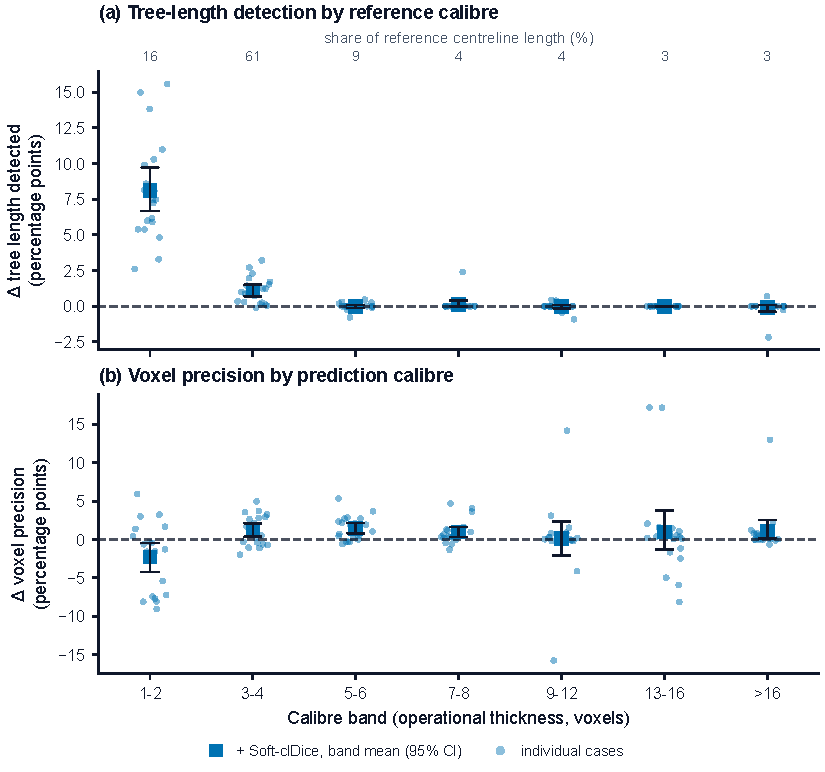
\includegraphics[width=\linewidth]{Figures/pdf/results/calibre_delta_td_noinset.pdf}
  \caption[Tree-length and precision changes by airway calibre]{Paired Soft-clDice minus
  comparator differences on the 20-case validation cohort. A: TLD stratified by reference
  calibre. B: voxel precision stratified by each prediction's own calibre because false-positive
  voxels have no reference calibre. Squares show band means with 95\% patient-bootstrap
  intervals; pale points show cases, and positive values favour Soft-clDice. The upper axis gives
  each band's share of reference centreline length.}
  \label{fig:calibre-delta}
\end{figure}

\begin{table}[htbp]
  \centering
  \footnotesize
  \setlength{\tabcolsep}{2pt}
  \caption[Tree length stratified by ground-truth airway calibre]{Tree length detected by local
  lumen calibre on the external validation cohort. Bands are the exhaustive operational classes
  of Equation~\eqref{eq:opclass}, and ``GT len'' is each band's share of annotated centreline
  length. ``Seed'' is the 16-label initial checkpoint and ``Sup. ref.'' the 110-label scale
  reference. TLD values are percentages and differences are percentage points.}
  \label{tab:calibre-td}
  \begin{tabular}{lrrrrrrrr}
    \toprule
    Thickness & GT len & Seed & Config. & MT & MT & Sup. & $\Delta$ MT & Wins \\
    (voxels) & (\%) & & & fold~0 & 5-fold & ref. & $-$ control & \\
    \midrule
    1--2   & 15.65 & 64.44 & 67.10 & \textbf{75.20} & 73.82 & 70.73 & $+$8.10$^{***}$ & 20/20 \\
    3--4   & 61.34 & 95.23 & 95.68 & 96.77 & \textbf{96.90} & 96.81 & $+$1.09$^{***}$ & 19/20 \\
    5--6   &  9.11 & 99.68 & 99.72 & 99.72 & 99.77 & \textbf{99.78} & 0.00 & 4/20 \\
    7--8   &  3.92 & 99.85 & 99.48 & 99.62 & 99.88 & \textbf{99.93} & $+$0.14 & 2/20 \\
    9--12  &  4.13 & 99.77 & 99.69 & 99.66 & 99.82 & \textbf{99.84} & $-$0.03 & 2/20 \\
    13--16 &  2.56 & 98.47 & 98.50 & 98.50 & 98.53 & \textbf{98.76} & 0.00 & 0/20 \\
    $>$16  &  3.29 & \textbf{96.20} & 96.06 & 95.95 & 94.53 & 93.57 & $-$0.11 & 1/18 \\
    \midrule
    All    & 100.00 & 91.34 & 92.02 & \textbf{93.98} & 93.81 & 93.33 & $+$1.96$^{***}$ & 20/20 \\
    \bottomrule
  \end{tabular}
  \parbox{\linewidth}{\footnotesize $^{***}p<0.001$, Wilcoxon signed-rank; unmarked
  differences $p>0.05$. The $>$16 band uses 18 cases because two contain no voxels in it.}
\end{table}

\begin{table}[htbp]
  \centering
  \footnotesize
  \setlength{\tabcolsep}{3pt}
  \caption[Voxel precision stratified by predicted airway calibre]{Voxel precision stratified by
  each prediction's own local calibre on the external validation cohort. Bands use the
  operational classes of Equation~\eqref{eq:opclass}; prediction-derived classes are required
  because false-positive voxels have no reference calibre. Values are patient-level means in
  percent and differences are percentage points. Arm abbreviations match
  Table~\ref{tab:calibre-td}.}
  \label{tab:calibre-precision}
  \begin{tabular}{lrrrrrrr}
    \toprule
    Thickness & Seed & Config. & MT & MT & Sup. & $\Delta$ MT & Wins \\
    (voxels) & & & fold~0 & 5-fold & ref. & $-$ control & \\
    \midrule
    1--2   & 76.43 & 76.11 & 73.82 & 76.42 & \textbf{78.75} & $-$2.29 &  6/20 \\
    3--4   & 91.56 & 92.42 & 93.69 & 93.91 & \textbf{93.93} & $+$1.27 & 13/20 \\
    5--6   & 94.12 & 94.72 & \textbf{96.19} & 95.74 & 96.05 & $+$1.47 & 15/20 \\
    7--8   & 94.84 & 95.39 & \textbf{96.38} & 96.16 & 96.35 & $+$0.99 & 17/20 \\
    9--12  & 95.87 & 96.28 & 96.42 & \textbf{97.08} & 96.67 & $+$0.14 & 14/20 \\
    13--16 & 95.96 & 95.05 & 96.01 & 95.54 & \textbf{98.43} & $+$0.96 & 14/20 \\
    $>$16  & 92.51 & 95.30 & \textbf{96.37} & 96.30 & 95.79 & $+$1.07 & 15/18 \\
    \bottomrule
  \end{tabular}
  \parbox{\linewidth}{\footnotesize ``Wins'' counts cases with higher precision under fold-0
  Soft-clDice than under the configuration comparator. The $>$16 band uses 18 complete cases;
  overall voxel precision is reported in Table~\ref{tab:primary-current}.}
\end{table}
\end{currentcontrolroute}
\fi

\ifshowpairedcontrol
\begin{pairedcontrolroute}
\noindent\textbf{Prospective paired-seed route.}
\pending[Replace the fitted-checkpoint display with seed-paired calibre differences and
across-seed intervals.]
\end{pairedcontrolroute}
\fi

\section{Airway-tree recovery by branch depth}
\label{sec:depth}

\ifshowcurrentcontrol
\begin{currentcontrolroute}
Figure~\ref{fig:depth-recovery} shows tree-length recovery by reference branch depth. The
fitted-checkpoint difference emerged beyond depth~3 on both validation and held-out cohorts.

\begin{figure}[htbp]
  \centering
  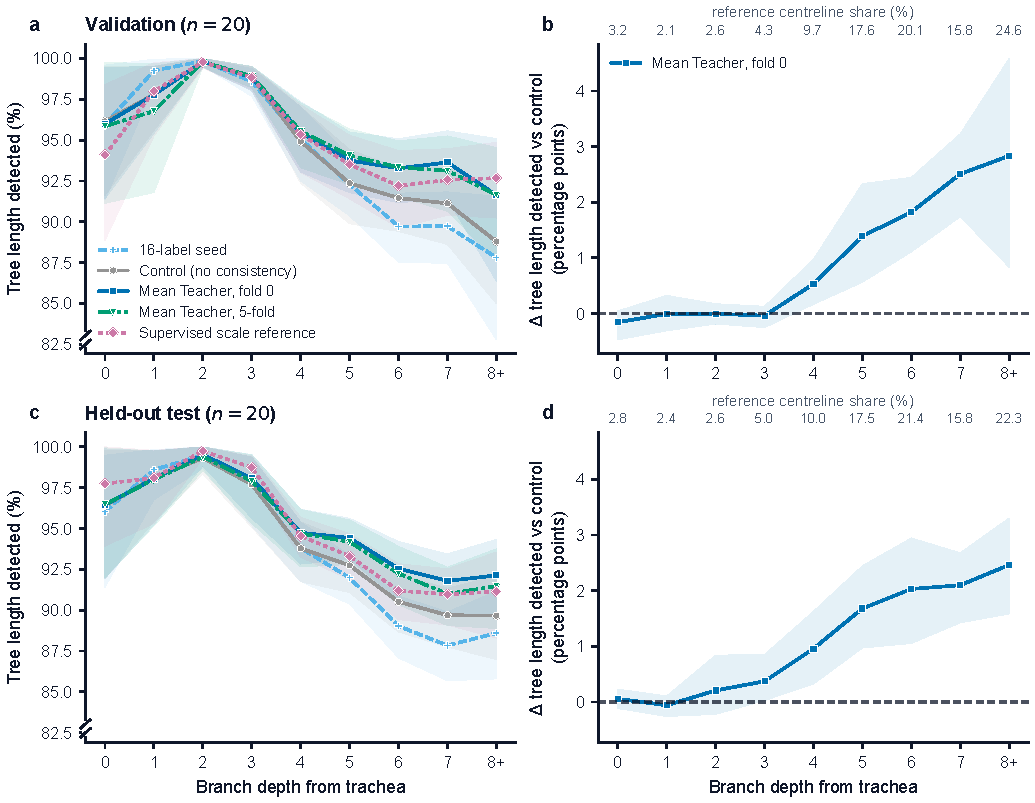
\includegraphics[width=\linewidth]{Figures/pdf/results/generation_depth_recovery.pdf}
  \caption[Tree-length recovery by branch depth]{Branch-depth recovery on the ATM'22 validation (a,b) and held-out test
(c,d) cohorts. Left: absolute tree-length detection percentages, including the 16-label seed
and 110-label scale reference. Right: paired percentage-point difference between the fold-0
Mean Teacher and its configuration-matched no-consistency comparator. Lines and shaded regions
show cohort means and 95\% bootstrap intervals over 20 cases. Depths eight and above are pooled
as $8+$.}
  \label{fig:depth-recovery}
\end{figure}
\end{currentcontrolroute}
\fi

\ifshowpairedcontrol
\begin{pairedcontrolroute}
\noindent\textbf{Prospective paired-seed route.}
\pending[Replace the fitted-checkpoint display with seed-paired depth differences and
across-seed intervals.]
\end{pairedcontrolroute}
\fi

\section{Secondary comparisons}
\label{sec:ablation-mse}
\label{sec:soft-fivefold}
\label{sec:ablation-weight}

\ifshowcurrentcontrol
\begin{currentcontrolroute}
The five-fold ensemble and voxel-MSE arm are included in
Table~\ref{tab:primary-current}.
\end{currentcontrolroute}
\fi
Table~\ref{tab:weight-sensitivity} reports the completed soft-clDice consistency-weight sweep.

\begin{table}[htbp]
  \centering
  \footnotesize
  \caption[Consistency-weight sensitivity]{Fold-0 validation sensitivity to the maximum
  soft-clDice consistency weight. Metrics are percentages. These are single runs;
  $w_{\max}=0.10$ is the reported operating point.}
  \label{tab:weight-sensitivity}
  \begin{tabular}{lrrrrrr}
    \toprule
    $w_{\max}$ & Dice & TLD & BD & Precision & TPrec. & clDice \\
    \midrule
    0.03 & 92.76 & 92.99 & 87.39 & 93.54 & 92.27 & 92.48 \\
    0.10 & 92.25 & 93.98 & 89.09 & 94.15 & 90.57 & 92.08 \\
    0.30 & 92.14 & 95.26 & 91.42 & 93.53 & 86.69 & 90.61 \\
    \bottomrule
  \end{tabular}
\end{table}

\section{External evaluation}
\label{sec:external}

\ifshowcurrentcontrol
\begin{currentcontrolroute}
Held-out ATM'22 and AeroPath performance is summarised in
Table~\ref{tab:external-evaluation}.

\begin{table}[htbp]
  \centering
  \footnotesize
  \setlength{\tabcolsep}{5pt}
  \caption[External evaluation]{Native-output performance on the sealed 20-case ATM'22 test
  cohort and the 27-case AeroPath cohort. Mean Teacher rows use the deployed EMA teacher.
  Metrics are percentages; differences are percentage points comparing fold~0 Mean Teacher
  with the no-consistency comparator.}
  \label{tab:external-evaluation}
  \begin{tabular}{lrrrrr}
    \toprule
    Arm & Dice & TLD & BD & Prec. & clDice \\
    \midrule
    \multicolumn{6}{l}{\itshape Sealed ATM'22 test cohort} \\
    Supervised scale reference & 92.58 & 92.69 & 86.98 & 93.14 & \textbf{92.17} \\
    16-label seed              & 91.84 & 90.63 & 83.14 & 92.11 & 90.86 \\
    No-consistency control     & 92.10 & 91.63 & 85.39 & 92.25 & 91.63 \\
    Mean Teacher, fold~0       & 92.01 & \textbf{93.44} & \textbf{89.18} & 93.30 & 91.47 \\
    Mean Teacher, five folds   & \textbf{92.93} & 93.01 & 88.22 & \textbf{94.19} & 92.00 \\
    $\Delta$ fold-0 MT $-$ control (pp) & $-$0.09 & $+$1.81 & $+$3.79 & $+$1.05 & $-$0.16 \\
    \addlinespace
    \multicolumn{6}{l}{\itshape AeroPath out-of-distribution cohort} \\
    Supervised scale reference & \textbf{84.95} & 94.59 & 92.03 & \textbf{86.28} & \textbf{80.74} \\
    No-consistency control     & 84.22 & 94.46 & 91.20 & 82.56 & 78.50 \\
    Mean Teacher, fold~0       & 84.24 & 95.03 & 92.52 & 83.99 & 76.18 \\
    Mean Teacher, five folds   & 84.90 & \textbf{95.41} & \textbf{92.73} & 84.67 & 77.76 \\
    \addlinespace
    $\Delta$ fold-0 MT $-$ control (pp) & $+$0.02 & $+$0.57 & $+$1.32 & $+$1.43 & $-$2.32 \\
    \bottomrule
  \end{tabular}
\end{table}
\end{currentcontrolroute}
\fi

\ifshowpairedcontrol
\begin{pairedcontrolroute}
\noindent\textbf{Prospective paired-seed route.}
\pending[Insert seed-paired external-evaluation table for held-out ATM'22 and AeroPath.]
\end{pairedcontrolroute}
\fi

% !TEX root = ../main.tex
% Chapter: Discussion
\chapter{Discussion}
\label{ch:discussion}

% Booklet brief: begin with a 1--2 sentence summary, interpret rather than repeat Results,
% compare objectively with literature, identify failures and limitations, and propose
% improvements. The working draft deliberately shows both control routes. Before submission,
% exactly one route must be enabled in main.tex.
% Target after the final whole-document cut: approximately 1,750 words including ethics and
% future work. Percentages and percentage points follow the convention used in Results.

\section{Principal findings and their meaning}

This study implemented geometry-aware Mean Teacher training for pulmonary airway segmentation
and tested whether unlabelled CT changed recovery of the airway tree rather than only voxel
overlap.

\ifshowcurrentcontrol
\begin{currentcontrolroute}
The fitted Mean Teacher recovered more thin and deep airway structure on validation and held-out
data while its Dice score remained broadly unchanged, but the unpaired training runs restrict
this to a fitted-checkpoint comparison.

Against the current configuration-matched comparator, validation TLD and BD increased by
1.96 and 3.62 percentage points, respectively, whereas Dice decreased by 0.39 points. The
held-out ATM'22 cohort showed differences of similar size (TLD $+1.81$, BD $+3.79$ and Dice
$-0.09$ points). This reproducibility across patients and cohorts suggests that the two fitted
models occupy different operating points, but it does not establish a training-method effect:
their output heads and stochastic training trajectories were independently realised.
\end{currentcontrolroute}
\fi

\ifshowpairedcontrol
\begin{pairedcontrolroute}
Across the completed pairs, Mean Teacher \pending[: increased/did not consistently increase]
thin and deep airway recovery while Dice \pending[: remained stable/changed]; this supports
\pending[: a repeatable training-method effect/a run-specific fitted-model difference].

Across \pending[: number] complete seed pairs, Mean Teacher changed TLD by \pending and BD by
\pending percentage points, with effects in the same direction in \pending and \pending pairs;
Dice changed by \pending points. Because each eligible pair shared its complete initial state and
stochastic schedule, this estimates a fold-0 training-method effect rather than a difference
between two selected checkpoints. It remains conditional on one labelled split and the completed
pairs available by the pre-specified deadline.
\end{pairedcontrolroute}
\fi

The useful result is therefore the emph{shape} of the change, not a claim that the model became
uniformly better. The calibre, branch-depth and error-type analyses together ask whether the
consistency term changed where the network committed foreground and what it sacrificed to do so.

\ifshowcurrentcontrol
\begin{currentcontrolroute}
On validation, the TLD difference was 8.10 points in one-to-two-voxel airways, compared with
1.09 points at three to four voxels and no significant difference above four voxels. After
weighting by each band's share of the reference centreline, the one-to-two-voxel class supplied
approximately 65\% of the total TLD difference and the three-to-four-voxel class supplied the
remainder. Independently, the difference was negligible through branch depths 0--3 and rose to
2.83 points in the pooled $8+$ tail. BD followed the same depth profile, suggesting that reference
branches crossed the 80\% detection criterion rather than only acquiring isolated foreground
voxels. Agreement between the two axes localises the fitted-model difference to peripheral
reference structure, but does not distinguish anatomically valid extension from thin-branch
over-segmentation.
\end{currentcontrolroute}
\fi

\ifshowpairedcontrol
\begin{pairedcontrolroute}
Across complete pairs, the mean TLD effect was \pending in one-to-two-voxel airways and \pending
above four voxels. It was \pending through branch depths 0--3 and \pending in the pooled distal
tail, with the peripheral pattern present in \pending[: number] of \pending[: number] pairs.
Agreement between calibre and depth would support a repeatable peripheral redistribution;
disagreement would preclude a consistent localisation claim.
\end{pairedcontrolroute}
\fi

Airway-specific work has likewise identified foreground imbalance, discontinuity and peripheral
branch loss as related but distinct problems~\cite{qin2019airwaynet,zheng2021gradient,
yu2022break,Nan2024FANN}. The present analysis adds localisation along two measured anatomical
coordinates, while the selected control route determines whether that pattern belongs only to
two fitted models or generalises across training runs.

The apparent disagreement between Dice and tree recovery follows directly from airway geometry.
The one-to-two-voxel class contains 15.65\% of annotated centreline length but only 3.31\% of
airway volume. The same imbalance appears topologically: depths 0--3 contain 66.2\% of annotated
volume but only 12.2\% of centreline length. A volume-weighted score can therefore remain almost
fixed while a length-weighted score changes in the peripheral 87.8\% of the tree
~\cite{dice1945association,zheng2021gradient,shit2021cldice,zhang2023atm22}.

\ifshowcurrentcontrol
\begin{currentcontrolroute}
The error decomposition makes the exchange more specific. In one-to-two-voxel airways, the
8.10-point TLD difference was almost twice the 4.54-point voxel-recall difference, while precision
within predictions assigned to that class fell by 2.29 points. Above two voxels, voxel recall
fell while TLD was retained and voxel precision increased. This is a redistribution towards
centreline reach with fewer retained voxels elsewhere; it is not evidence that anatomical wall
thickness improved. Higher TLD is also insufficient by itself: a dilated or false-positive
extension that overlaps the reference centreline can raise coverage while creating an invalid
route. The fitted model therefore moved towards peripheral completeness at a bounded thin-branch
precision cost, rather than improving every part of the mask.

Whole-tree surfaces remain difficult to compare because most prediction voxels are shared.
Figure~\ref{fig:supp-qualitative} therefore traces one change across three scales. ATM~087 was
selected before rendering as the largest patient-level paired TLD gain, making it an illustrative
mechanistic best case rather than a representative patient. Panel A localises the change on the
whole tree; Panel B isolates the same region in 3-D; and Panel C places the selected component on
the underlying CT and reference annotation. The component was selected automatically before
visual inspection as the largest connected, thin and elongated annotated volume present only
under Soft-clDice. It spans 12.3~mm along its long axis, contains 83 newly correct foreground
voxels and accounts for 18 Soft-clDice-only reference-centreline voxels. Thus the patient-level
TLD improvement can, in this example, be spatially attributed partly to a coherent
reference-supported addition rather than merely to a diffuse change in segmentation overlap.
Preserving such distal paths is relevant to airway morphometry and navigation
~\cite{Wang2023qct,Dhillon2017PeripheralBronchoscopy,HammadAltaq2023robotic}, but this example does
not show that Soft-clDice generally restores distal branches, nor does it establish downstream
connectivity, bronchoscopic traversability or clinical benefit.
\end{currentcontrolroute}

\begin{figure}[p]
  \centering
  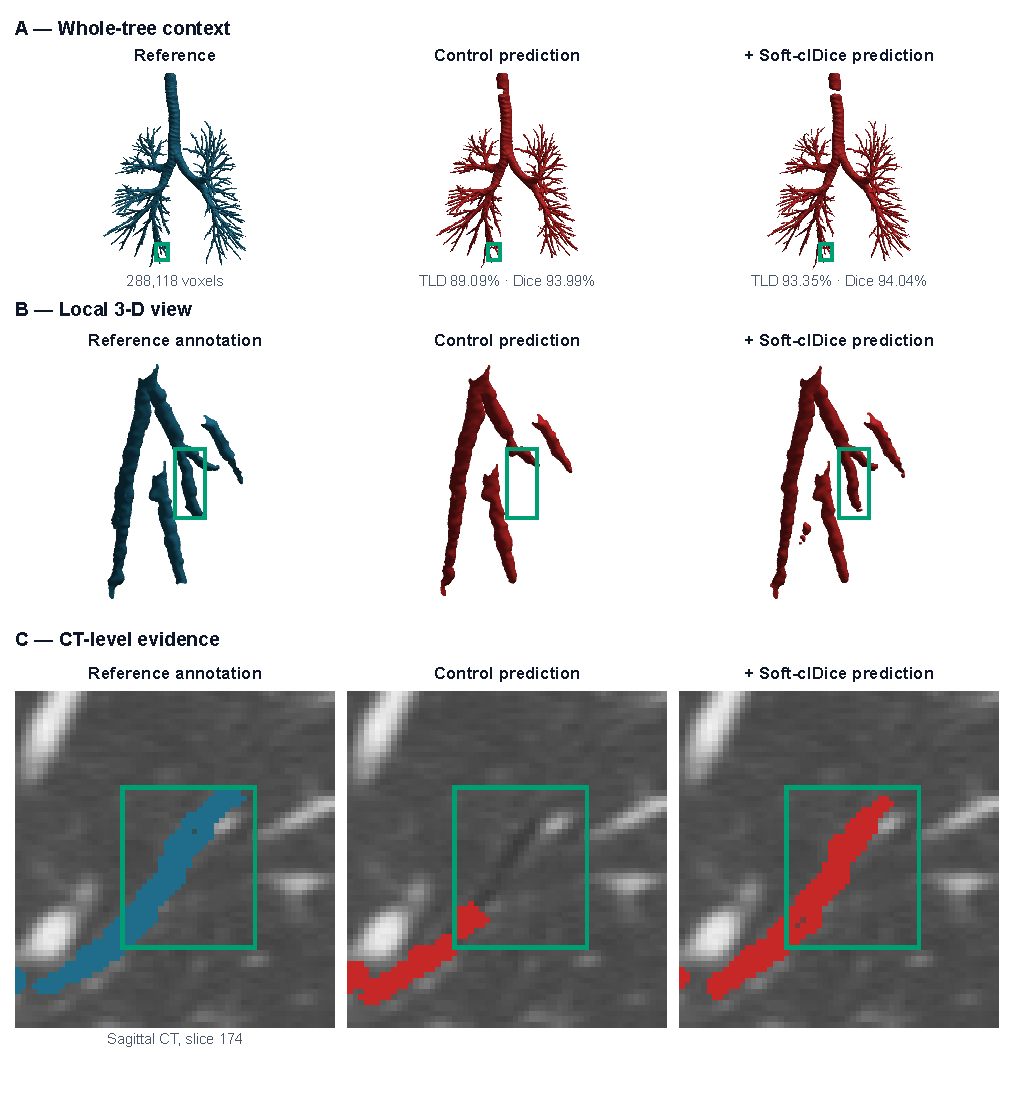
\includegraphics[width=\linewidth,height=0.79\textheight,keepaspectratio]{Figures/pdf/discussion/qualitative_plate_val_087.pdf}
  \caption[Multiscale localisation of a reference-supported addition]{Illustrative mechanistic
  best case, not cohort-level evidence. ATM~087 was selected before rendering as the largest
  patient-level paired TLD gain ($89.09\%$ to $93.35\%$; $+4.26$ percentage points). A gives
  whole-tree context and boxes the region; B enlarges the same 3-D segment; C shows its location on
  sagittal CT. Each row has the same order: reference annotation, control prediction and
  Soft-clDice prediction. Blue denotes the reference mask, red the model predictions, and green
  boxes identify the same region rather than an additional segmentation class. The automatically
  selected component contains 83 foreground and 18 centreline voxels and spans 12.3~mm. It
  spatially explains part of this patient's TLD difference but does not establish generally
  recovered anatomy or clinical utility.}
  \label{fig:supp-qualitative}
\end{figure}
\fi

\ifshowpairedcontrol
\begin{pairedcontrolroute}
Across complete pairs, voxel precision changed by \pending overall and by \pending in the
one-to-two-voxel class, while centreline precision changed by \pending. These results support
\pending[: a repeatable shift towards peripheral completeness/a less stable recall--precision
trade-off], rather than uniform improvement.
\end{pairedcontrolroute}
\fi

\section{Why the change localised to thin and deep airways}

The loss supplies the first part of a mechanistic explanation. Voxelwise MSE in
Equation~\eqref{eq:lmse} counts every cross-sectional voxel, so wide proximal structures can
contribute more disagreement than a narrow branch of the same length. By contrast, the
directional terms of Equation~\eqref{eq:tterms} normalise against soft-skeleton mass. Soft-clDice
has improved connectivity in tubular segmentation~\cite{shit2021cldice}; related semi-supervised
airway and vessel work likewise replaces plain voxel agreement with specialised or cross-geometry
representations~\cite{gu2023featurespecialisation,zhu2024crossgeometry}. The claim here is narrower
than the topological guarantee proved for binary masks: finite soft morphology on probability maps
neither enforces one connected airway tree nor establishes that a predicted branch is
anatomically correct.

The implementation introduces a more specific effect. As Figure~\ref{fig:soft-skeleton-iteration}
shows, a structure at most two voxels across is annihilated by the first cross erosion. Its opening
is then zero and the depth-zero residual equals the entire probability structure, rather than an
ideal one-voxel centreline. In the implementation-matched probe, the one-to-two-voxel class
formed 9.47\% of sampled teacher foreground but 28.69\% of teacher soft-skeleton mass: a
threefold relative representation. The apparent defect therefore does not suppress the thinnest
tree. It acts as an accidental thin-structure weighting, summarised in
Figure~\ref{fig:discussion-mechanism}.

\begin{figure}[htbp]
  \centering
  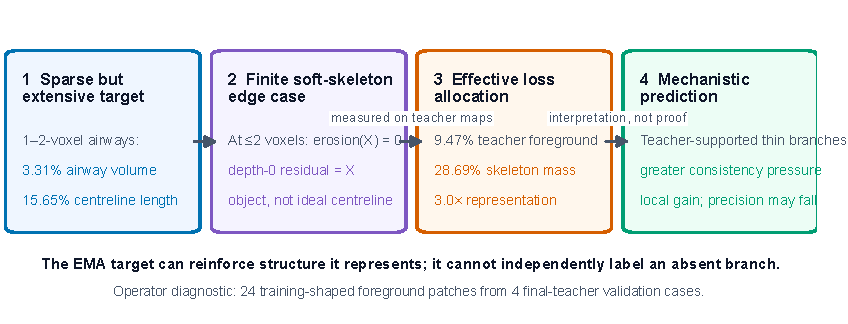
\includegraphics[width=\linewidth]{Figures/pdf/discussion/mean_teacher_mechanism.pdf}
  \caption[Mechanistic account of the thin-airway effect]{Implementation-matched account of how
  thin airways acquire leverage in the consistency loss. The target census uses the 20-case
  validation cohort. The loss-allocation diagnostic uses 24 training-shaped, foreground-centred
  patches sampled from four final EMA-teacher probability maps. Solid arrows join definitions or
  measurements; the dashed arrow is a mechanistic interpretation, not causal proof. The predicted
  localisation is tested independently by the calibre and depth results in
  Figures~\ref{fig:calibre-delta} and~\ref{fig:depth-recovery}.}
  \label{fig:discussion-mechanism}
\end{figure}

The same probe explains why twofold upsampling is not an automatic repair. Upsampling reduced
the fraction of teacher foreground annihilated by one erosion from 34.03\% to 20.39\% and reduced
total skeleton mass from 8.78\% to 3.07\% of foreground, so it produced a geometrically thinner
skeleton. However, the thinnest class still received 25.89\% of skeleton mass, compared with
28.69\% at native resolution, while a checkpointed consistency pass increased from approximately
0.16 to 3.10 seconds. It changes the skeleton's magnitude far more than the relative allocation
that drives the normalised sensitivity term. A full upsampled training arm could therefore spend
substantial compute while also weakening the accidental weighting associated with the primary
effect; geometric correctness alone does not predict a better fitted model.

\ifshowcurrentcontrol
\begin{currentcontrolroute}
The predicted signature is present: this class produced the largest fitted-model TLD difference
in all 20 validation cases and approximately 65\% of the aggregate difference. The concordance
between an implementation-derived prediction and a separately measured outcome supports the
weighting mechanism, although the post-hoc probe and unpaired checkpoints do not identify it
causally.
\end{currentcontrolroute}
\fi

\ifshowpairedcontrol
\begin{pairedcontrolroute}
The paired effect was \pending[: largest/not consistently largest] in this class, which
\pending[: supports/does not support] thin-structure weighting as a repeatable mechanism.
\end{pairedcontrolroute}
\fi

Neither route shows that differentiable skeletonisation preserved topology for its intended
mathematical reason. This distinction is important because
recent airway methods obtain structural gains through different mechanisms, including
connectivity-aware learning, feature specialisation and multi-task topology enhancement
~\cite{qin2019airwaynet,gu2023featurespecialisation,yang2024topoenhance}.

Calibre does not, however, explain the entire spatial pattern. Across the reference centreline,
branch depth and calibre were only moderately correlated ($\rho=-0.48$): 94.3\% of the
one-to-two-voxel centreline lay at depth~5 or deeper, but 81.0\% of the depth-$\geq5$ centreline
was wider than two voxels. Thus ``thin'' usually means peripheral, but ``peripheral'' does not
mean only the thinnest class.

\ifshowcurrentcontrol
\begin{currentcontrolroute}
Descriptively, the fitted TLD difference still increased with depth within the fixed
one-to-two- and three-to-four-voxel bands ($\rho=0.78$ and $0.98$). The 110-label supervised
reference showed the same depth-graded shape at smaller magnitude through depths 4--7. The
location is therefore a general signature of improving peripheral recovery, while the
soft-skeleton weighting plausibly helps set its magnitude.
\end{currentcontrolroute}
\fi

\ifshowpairedcontrol
\begin{pairedcontrolroute}
Within fixed calibre bands, the across-pair TLD effect changed with depth by \pending. A retained
depth trend would support a spatial effect beyond calibre; its absence would restrict the
mechanistic account to thin-structure weighting.
\end{pairedcontrolroute}
\fi

This remaining depth association is plausibly produced by the interaction between the target and
the data. Peripheral lumina approach the acquisition resolution, so partial-volume effects and
weak contrast make their predictions less stable under intensity perturbation
~\cite{montaudon2007,GarciaUceda2021AirwayCNN}. EMA averaging supplies a temporally smoother target
~\cite{tarvainen2017mean,laine2017temporal,yu2019uamt}; consistency can therefore discourage the
student from intermittently dropping a weak branch that the teacher already represents. It does
not encode branch depth explicitly, so this remains an evidence-consistent explanation rather
than a learned anatomical-depth mechanism.

The consistency-weight sweep explains why gains in tree recovery are accompanied by losses
elsewhere. Increasing $w_{\max}$ from 0.03 to 0.30 monotonically increased TLD and BD, but topology
precision fell from 92.27\% to 86.69\% and the corresponding evaluation clDice fell from 92.48\%
to 90.61\% (Table~\ref{tab:weight-sensitivity}). A larger weight therefore made the network commit
to more reference centreline while accepting more unsupported predicted centreline. This is an
operating-point curve, not monotonic improvement, and no turning point was bracketed.

\ifshowcurrentcontrol
\begin{currentcontrolroute}
Only $w_{\max}=0.10$ has five-fold, held-out and out-of-distribution evaluation.
\end{currentcontrolroute}
\fi

\ifshowpairedcontrol
\begin{pairedcontrolroute}
The seeded programme fixes $w_{\max}=0.10$; the other weights remain single-run sensitivity
points and do not estimate variation in the weight response.
\end{pairedcontrolroute}
\fi

\ifshowcurrentcontrol
\begin{currentcontrolroute}
The voxel-MSE arm at $w_{\max}=0.30$ remained close to the configuration comparator. This is
consistent with the proposed normalisation account: Equation~\eqref{eq:lmse} averages disagreement
over the patch, whereas Equation~\eqref{eq:tterms} allocates it through skeleton mass. Similar
concerns motivate geometry- and distance-consistency methods for tubular targets
~\cite{gu2023featurespecialisation,zhu2024crossgeometry,zhao2025vesselselftraining}. It is not
controlled proof that soft-clDice is superior, because the objectives were not weight-matched and
their gradient scales differ.
\end{currentcontrolroute}
\fi

\ifshowpairedcontrol
\begin{pairedcontrolroute}
The existing voxel-MSE result is not part of the seeded treatment contrast: it is one run at
$w_{\max}=0.30$ without an identical-state MSE--control pair. It therefore provides descriptive
evidence about that fitted objective, not an across-seed comparison with soft-clDice.
\end{pairedcontrolroute}
\fi

A matched plain and foreground--background-balanced MSE comparison is needed before attributing
the result specifically to centreline geometry.

The mechanism also explains why stronger consistency eventually loses precision. The target is
an EMA model, not the reference annotation. If a teacher extension is stable but anatomically
wrong, increasing its weight makes the student more consistent with that error; this is analogous
to confirmation bias in pseudo-label learning~\cite{arazo2020confirmation}. Conversely, Mean
Teacher cannot provide independent positive evidence for a branch wholly absent from the teacher.
EMA averaging can stabilise a represented branch under perturbation
~\cite{tarvainen2017mean,laine2017temporal,yu2019uamt}, but teacher and student errors remain
correlated. Supervised gradients may still let the student exceed its teacher, so this is an
information constraint rather than an absolute ceiling.

That constraint is stronger in the implemented experiment because ordinary spatial augmentation
was shared between the two streams; only the additional intensity scale, shift and noise of
Equation~\eqref{eq:perturbation} separated them. The unlabelled signal therefore tests whether an
existing structure survives photometric perturbation, not whether two independent anatomical
views discover the same branch. This makes consolidation of weak teacher-supported evidence a
more likely explanation than anatomical discovery. Feature-specialised peers and task-level
cross-geometry consistency are credible alternatives precisely because they create more distinct
representations~\cite{gu2023featurespecialisation,zhu2024crossgeometry}.

\section{Robustness and relation to prior work}

\ifshowcurrentcontrol
\begin{currentcontrolroute}
Five-fold ensembling improved the balance between volumetric and topology-aware metrics and
removed the severe connected-component failure observed in one fold. It is the preferred
absolute deployment estimate, but the absence of a five-fold control means that it cannot be
used as a second treatment contrast. Similarly, the supervised model trained from a 110-case
pool supplies label-scale context rather than a ceiling or causal comparator: it differs in
training cases and pipeline. The fact that several Mean Teacher models exceed it in TLD while
not uniformly exceeding Dice or precision reinforces the need to report complementary measures,
as adopted by ATM'22~\cite{zhang2023atm22}.
\end{currentcontrolroute}
\fi

\ifshowcurrentcontrol
\begin{currentcontrolroute}
The fitted-model TLD and BD ordering persisted on held-out ATM'22 data and was attenuated on
AeroPath. This is evidence of retrospective robustness rather than clinical generalisability.
\end{currentcontrolroute}
\fi

\ifshowpairedcontrol
\begin{pairedcontrolroute}
The mean paired effect changed from \pending on validation to \pending on held-out ATM'22 and
\pending on AeroPath, retaining its direction in \pending and \pending complete pairs. This
provides \pending[: cross-cohort support/no stable external support] for the fold-0 effect.
\end{pairedcontrolroute}
\fi

AeroPath was designed to include pathology that challenges airway segmentation
~\cite{stoverud2023aeropath}, but acquisition spacing, annotation policy and case mix differ, so
absolute voxel-calibre bands are not directly transferable. Published semi-supervised airway
studies also use different labelled fractions, cohorts and baselines
~\cite{gu2023featurespecialisation,zhu2024crossgeometry}; numerical ranking against them would
therefore confound method with data and evaluation. The more useful comparison is conceptual:
all treat peripheral airway structure as a problem that conventional voxel consistency does not
fully represent, while this study additionally exposes how sensitive that conclusion is to the
choice of control.

\section{Limitations and improvements}

\ifshowcurrentcontrol
\begin{currentcontrolroute}
The dominant limitation is unmeasured training variation. Patient-paired tests and bootstrap
intervals quantify variation across evaluation cases conditional on two checkpoints; they do not
include variation from initialisation, data order, augmentation, GPU execution or labelled fold.
The present comparison should therefore be called a configuration contrast. Identical-state,
seed-paired control--Mean Teacher continuations are the direct improvement.
\end{currentcontrolroute}
\fi

\ifshowpairedcontrol
\begin{pairedcontrolroute}
Seed pairing measures training variation only for fold~0. It does not cover different labelled
splits, hardware or unpaired failures, and \pending[: number] completed pairs provide limited
precision for an across-seed effect. Replicating complete pairs on the remaining folds is the
direct improvement.
\end{pairedcontrolroute}
\fi

Each primary fold trained with 16 labelled patients, so augmentation increases the number of
views but not anatomical diversity. The held-out ATM'22 cohort is also not pristine confirmation:
historical development models had accessed it before the present comparison was frozen. AeroPath
adds a second case distribution, but neither cohort establishes performance across scanners,
institutions or demographic groups. Multicentre evaluation with metadata-defined subgroups is
required before making a population-level claim.

The unlabelled-pool experiment also did not isolate data quantity. Expanding the pool from 90 to
240 scans under 125{,}000 unlabelled draws reduced mean exposure from 1{,}388.9 to 520.8 draws per
scan. Increasing the number of unlabelled patches then changed compute as well as exposure. The
observed differences therefore cannot show whether the additional 150 scans lacked useful
information; a smaller-pool arm with matched exposure is the missing comparison.

Measurement introduces further uncertainty. TLD and BD depend on skeletonisation, junction
handling and an in-house branch parser that has synthetic tests but no golden parity test against
the official ATM'22 evaluator. Depth is a graph-derived branching order rather than Weibel
generation~\cite{weibel1963morphometry,tschirren2005airway,palagyi2006airway}. Centreline geometry is used both in the
training objective and in several outcomes, so Dice and precision remain necessary independent
checks. Reference annotations are themselves limited by CT resolution and annotation policy in
the distal tree; an additional plausible branch cannot be assumed correct simply because it
looks anatomically continuous. Finally, connected-component filtering can delete a genuine
subtree after one proximal break. Treating native output as primary and connected output as a
declared sensitivity makes that failure visible rather than averaging it away.

\section{Ethical considerations}

Engineering guidance places honesty, accuracy, public safety and communication of uncertainty at
the centre of professional practice~\cite{engineeringcouncil2026ethics}. For this study,
scientific integrity requires disclosure that a sampler fault invalidated an early arm and that
negative ablations were retained.

\ifshowcurrentcontrol
\begin{currentcontrolroute}
The configuration comparator is not a seeded causal control, and the current checkpoints cannot
be reproduced bit-for-bit. Integrity therefore rests on disclosing those limits rather than
hiding them behind patient-paired statistics.
\end{currentcontrolroute}
\fi

\ifshowpairedcontrol
\begin{pairedcontrolroute}
The prospective pairs pre-specify complete initial states, seeds, eligibility and checkpoint
policy. Integrity requires reporting incomplete pairs and deviations as well as successful runs;
pairing does not remove uncertainty from labelled fold, hardware or scoring provenance.
\end{pairedcontrolroute}
\fi

Configurations, code versions and machine-readable outputs improve reproducibility. Thresholds,
checkpoints and post-processing should not be selected after inspecting the desired outcome. This
follows Imperial's principles of integrity, proportional risk, beneficence and non-maleficence
~\cite{imperial2025ethicalframework}.

No new participant or animal was recruited, scanned or exposed to an intervention. ATM'22 and
AeroPath are public secondary datasets whose publishers describe their data provenance
~\cite{zhang2023atm22,stoverud2023aeropath}. Nevertheless, public availability does not remove
duties of confidentiality, licence compliance and purpose-limited use. Case examples should
remain anonymised, and any redistribution must follow each dataset's licence or access agreement.
The people represented in the training data are also not necessarily those who would bear deployment errors, so aggregate
performance cannot establish distributive fairness.

The direction of error matters clinically. A false-negative branch could hide a possible route,
whereas a confident false-positive branch could suggest a bronchoscopic path that does not exist
~\cite{Dhillon2017PeripheralBronchoscopy,HammadAltaq2023robotic}. A visually plausible tree may
encourage automation bias, particularly when connected-component processing converts a broken
prediction into a clean-looking but incomplete result. WHO guidance consequently emphasises
human oversight, accountability, inclusiveness and continuing evaluation for health AI
~\cite{who2021aiguidance}; software used for clinical decisions would also require an appropriate
medical-device evidence and governance pathway~\cite{mhra2025aimd}. The present models should
therefore remain research tools unless prospectively validated with clinician oversight,
failure warnings and application-specific acceptance criteria.

Computational cost is also an ethical trade-off. Retained logs account for at least 356 GPU-hours,
excluding failed, missing and queued jobs, so this is a lower bound rather than metered total
energy. Carbon estimates depend on accelerator power, host memory, data-centre efficiency and grid
intensity~\cite{lannelongue2021green}. Pre-specifying a limited number of paired runs, reusing
saved predictions for secondary analyses and publishing negative results reduce avoidable
repetition; the final
report should replace this floor with the scheduler-derived total.

\section{Future work}

\ifshowcurrentcontrol
\begin{currentcontrolroute}
The first priority is to complete identical-state control--Mean Teacher seed pairs and then
replicate them across labelled folds. Until then, additional performance tuning cannot repair the
main inferential weakness.
\end{currentcontrolroute}
\fi

\ifshowpairedcontrol
\begin{pairedcontrolroute}
With fold-0 seed variation estimated, the first priority is complete-pair replication across
labelled folds and external cohorts. This tests whether the effect survives a different labelled
sample rather than only a different training trajectory.
\end{pairedcontrolroute}
\fi

The next ablations should separate mechanisms rather than add an undirected sweep. First, plain
and foreground--background-balanced MSE must be compared at the same $w_{\max}$ and initial state
as soft-clDice. Extending the consistency-weight range is useful only until it brackets a turning
point or collapse; replication at a selected weight is then more informative than adding rungs.
Second, changing the soft-skeleton iteration depth from the reported $K=10$ can test the finite
representation of wider structures, but it cannot remove the depth-zero edge case that weights
one-to-two-voxel branches. It is therefore a secondary ablation, not a direct test of the primary
mechanism. A direct test would alter the iteration-zero contribution, or compare native and
upsampled skeletonisation at a shared initial state, then ask whether the thin-band effect weakens
as predicted. The existing twofold probe shows that upsampling repairs the morphology at an
approximately twentyfold per-pass time cost while leaving relative thin-band allocation similar;
a full arm is justified only if that mechanistic question outweighs seed replication. A 90-scan
arm with unlabelled exposure matched to the 240-scan arm would separately estimate the value of
pool size.

The central information constraint requires a different experiment. Replacing the EMA target
temporarily with a more fully supervised teacher would distinguish teacher capacity from the
consistency mechanism, although it would be a diagnostic that imports label information rather
than a deployable semi-supervised method. Independently initialised peers, or a segmentation and
distance-transform dual head with cross-geometry and Hausdorff consistency, could then introduce
genuinely different representations~\cite{zhu2024crossgeometry}. A fully supervised 260-label
model would strengthen label-scale context but would still not replace the matched continuation
control. Finally, metric parity testing and prospective multicentre, clinician-facing evaluation
are prerequisites for anatomical or clinical claims.

% !TEX root = ../main.tex
% Chapter: Conclusion
\chapter{Conclusion}
\label{ch:conclusion}

% One paragraph (booklet: "1 paragraph"): the take-home message and how the findings could
% be used or explored further. May instead be folded into the final paragraph of the
% Discussion -- if so, delete this chapter and its \include in main.tex.
%
% REWIRED 2026-08-14: the take-home is now about what teacher-derived consistency can and
% cannot supply on a sparse tubular target, and about the value of measuring the mechanism
% rather than reporting the delta. Do NOT reintroduce the from-scratch or retired-loss conclusions.
%
% ROUGH-DRAFT CONTENT: condense these bullets into one final paragraph.
% FINAL WORD BUDGET: 150 words.
\begin{itemize}
  \item Opening claim: geometry-aware consistency makes semi-supervised training on sparse
  airway foreground numerically viable where per-voxel consistency does not, contributing on
  the order of 15\% of gradient norm without class balancing and without collapsing the
  teacher.
  \item[] \textcolor{red}{\textbf{This should be changed to:} Do not describe voxel-MSE as
  numerically non-viable. The completed $w_{\max}=0.30$ run trained and scored normally but
  remained close to, and slightly below, the no-consistency comparator. The defensible distinction
  is outcome and anatomical localisation; finalise it after the matched $w_{\max}=0.10$ arm is
  scored.}
  \item PLACEHOLDER --- the measured outcome against the exactly matched control, stated in
  one clause with its direction (completeness versus precision) and its single-seed bound.
  \item[] \textcolor{red}{\textbf{This should be changed to:} state the measured outcome
  against the configuration-matched no-consistency comparator and explicitly bound it to one
  independently initialised run per configuration. Conclude that the pattern is consistent
  with a consistency benefit, not that the comparison identifies a causal method effect.}
  \item Include the completed deployment estimate: the five-fold Mean Teacher ensemble
  retained the fold-0 topology result (TLD 0.9381, BD 0.8893) while improving Dice to 0.9277 and
  precision to 0.9455. Present this as absolute robustness across folds, not as a second controlled
  effect because no five-fold no-consistency ensemble was evaluated.
  \item The bounding insight, which is the part worth remembering: consistency redistributes
  the operating point but supplies no positive target for a branch the teacher never
  represents, so the achievable gain is set by teacher content rather than by the loss.
  \item Method-level take-home for the field: report semi-supervised results against a
  continuation control, separate unlabelled pool size from unlabelled exposure, and instrument
  the consistency term --- otherwise a null is uninterpretable and a gain is unattributable.
  \item Closing line: topology-aware measurement should be standard for airway models, and
  teacher-derived supervision is a targeted operating-point tool rather than a substitute for
  annotation.
\end{itemize}


%----------------------------------------------------------------------------------------
%	THESIS CONTENT - APPENDICES
%----------------------------------------------------------------------------------------

%TC:ignore  (appendix is not counted toward the 6000-word limit)
\appendix % Cue to tell LaTeX that the following "chapters" are Appendices

% !TEX root = ../main.tex
% Appendix A
\chapter{Supplementary Material}
\label{AppendixA}

% REWIRED 2026-08-14. This appendix now carries everything displaced from the body by the
% Mean Teacher rewire: the from-scratch MONAI study and the retired ablations. The
% appendix is NOT word-counted, so it is the right home for that material -- but it is still
% read, so it must stay accurate and must not contradict the body.
%
% ROUGH DRAFT: split into further appendices if navigation suffers.

\section{Dataset manifests}

\begin{itemize}
  \item Exact ATM'22 identifiers in the labelled, label-withheld, external validation and
  sealed test partitions, plus the split-generation seed and code version.
  \item Record that the split is a frozen manifest rather than a re-runnable splitter, and
  show the consequence: re-running the original count-based splitter over the enlarged
  inventory would have moved most previously held-out cases into training. Give the numbers.
  \item Declare which identifiers were added to the unlabelled pool only, and confirm no
  validation or test case entered any training pool.
  \item nnU-Net internal fold membership listed separately from the external project split,
  including the exact four-case internal validation set per fold.
  \item AeroPath case identifiers, with confirmation of external-evaluation-only use.
\end{itemize}

\section{Loss and objective definitions}

\begin{itemize}
  \item Full equations: weighted cross-entropy, soft Dice, differentiable skeletonisation,
  topology sensitivity, topology precision, soft clDice, and the consistency term as
  $1-F_1$ of the two directional terms at smoothing constant one.
  \item Document numerical stabilisers, erosion depth, pooling kernels, reduction over batch
  and channel dimensions, and the exact accumulation of ridge residuals.
  \item Derive and state the property referenced in the Discussion: for fractional maps the
  unthresholded objective is not zero at equality, hence a residual sharpening component.
  Show the algebra --- this is a load-bearing claim, so it should end in a result rather than
  a gesture.
\end{itemize}

Algorithm~\ref{alg:soft-skeleton} gives the skeletonisation of
Equations~\eqref{eq:morph}--\eqref{eq:accumulate} in the form it is implemented, with the
pooling kernels and the accumulation order made explicit.

\begin{algorithm}[htbp]
  \caption[Differentiable soft skeletonisation]{Differentiable soft skeletonisation, after Shit
  et al.~\cite{shit2021cldice}. \textsc{MinPool} and \textsc{MaxPool} are unit-stride pooling
  with shape-preserving padding; the three directional minimum pools compose to the
  six-neighbour erosion of Equation~\eqref{eq:morph}, and the cubic maximum pool is the
  26-neighbour dilation. Every operation is differentiable, so gradient reaches $X$ through each
  retained residual. Called on the student probability map and on the thresholded teacher tree
  with $K=10$.}
  \label{alg:soft-skeleton}
  \begin{algorithmic}[1]
    \Require probability map $X\in[0,1]^{D\times H\times W}$, erosion depth $K$
    \Ensure soft skeleton $S\in[0,1]^{D\times H\times W}$
    \Function{Erode}{$X$}\Comment{$\mathcal{E}$}
      \State \Return $\min\!\big(\textsc{MinPool}_{3\times1\times1}(X),\,
                                 \textsc{MinPool}_{1\times3\times1}(X),\,
                                 \textsc{MinPool}_{1\times1\times3}(X)\big)$
    \EndFunction
    \Function{Open}{$X$}\Comment{$\mathcal{O}=\mathcal{D}\circ\mathcal{E}$}
      \State \Return $\textsc{MaxPool}_{3\times3\times3}(\Call{Erode}{X})$
    \EndFunction
    \Statex
    \State $S \gets \operatorname{ReLU}\!\left(X-\Call{Open}{X}\right)$
      \Comment{$\delta^{(0)}$, Equation~\eqref{eq:residual}}
    \For{$k \gets 1$ \textbf{to} $K$}
      \State $X \gets \Call{Erode}{X}$ \Comment{$X^{(k)}$}
      \State $\delta \gets \operatorname{ReLU}\!\left(X-\Call{Open}{X}\right)$
        \Comment{$\delta^{(k)}$}
      \State $S \gets S+\operatorname{ReLU}\!\left(\delta-S\,\delta\right)$
        \Comment{probabilistic union, Equation~\eqref{eq:accumulate}}
    \EndFor
    \State \Return $S$
  \end{algorithmic}
\end{algorithm}

Figure~\ref{fig:soft-skeleton-operator} states the operator geometry that the main-text
figure demonstrates but cannot show: the two structuring neighbourhoods are different shapes,
so the composition is the implemented soft opening and not an adjoint morphological pair.
Figure~\ref{fig:soft-skeleton-extended} then expands the main-text illustration to show
intermediate erosion depths on a second patch. All panels are computed from three-dimensional
probability crops; only their presentation is two-dimensional.

\begin{figure}[htbp]
  \centering
  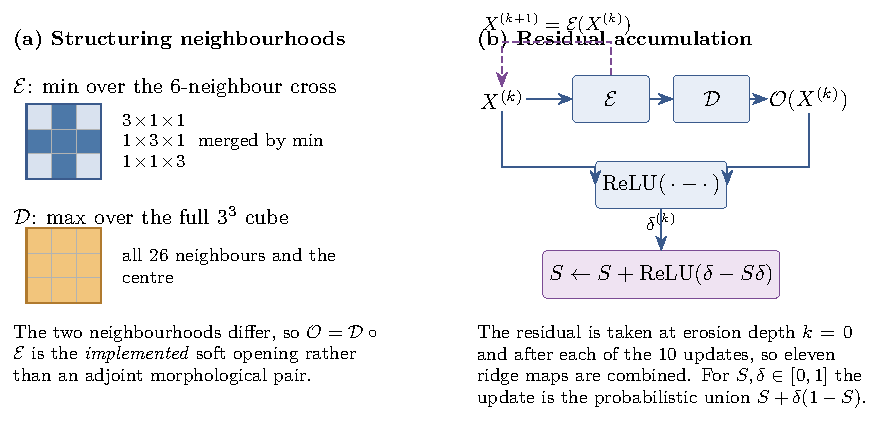
\includegraphics[width=\linewidth]{Figures/pdf/methods/cldice/soft_skeleton_operator.pdf}
  \caption[Soft-skeletonisation operators]{The implemented soft skeleton.
  (a)~Erosion takes the minimum over the six face-connected neighbours and the centre, built
  from three directional minimum pools; dilation takes the maximum over the full $3^3$ cube.
  (b)~Each erosion depth contributes the positive residual left by the opening, and the
  residuals are combined by a probabilistic union so that evidence is not double-counted.
  Operator geometry and dataflow only; no patient data is shown.}
  \label{fig:soft-skeleton-operator}
\end{figure}

\begin{figure}[htbp]
  \centering
  \begin{subfigure}[t]{0.32\textwidth}
    \centering
    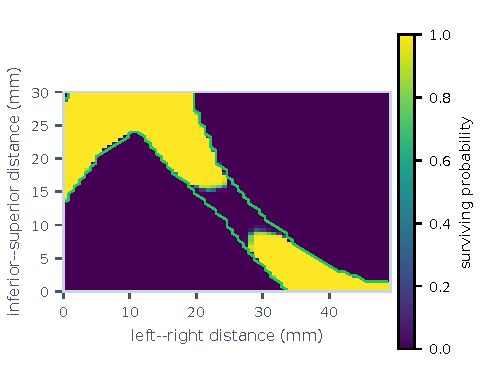
\includegraphics[width=\linewidth]{Figures/pdf/methods/cldice/soft_erosion_depth_0.pdf}
    \caption{Depth 0.}
  \end{subfigure}\hfill
  \begin{subfigure}[t]{0.32\textwidth}
    \centering
    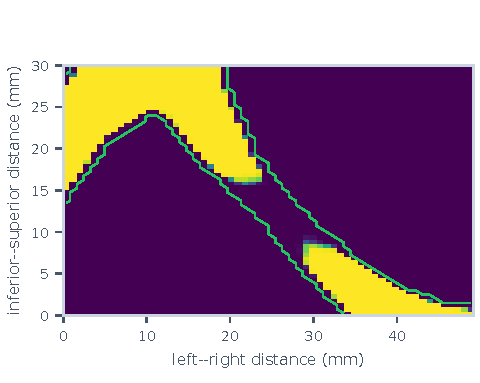
\includegraphics[width=\linewidth]{Figures/pdf/methods/cldice/soft_erosion_depth_1.pdf}
    \caption{Depth 1.}
  \end{subfigure}\hfill
  \begin{subfigure}[t]{0.32\textwidth}
    \centering
    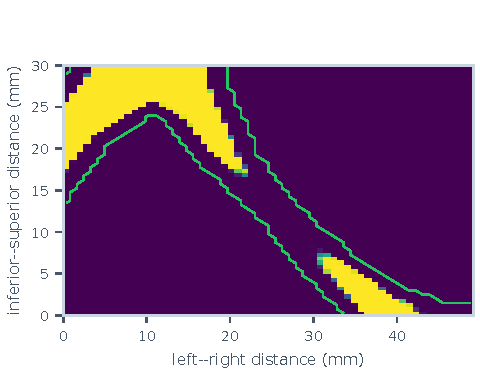
\includegraphics[width=\linewidth]{Figures/pdf/methods/cldice/soft_erosion_depth_3.pdf}
    \caption{Depth 3.}
  \end{subfigure}

  \medskip
  \begin{subfigure}[t]{0.32\textwidth}
    \centering
    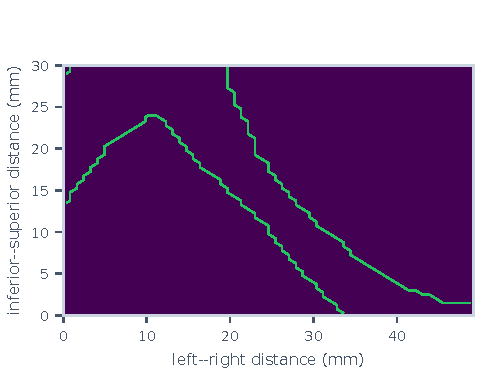
\includegraphics[width=\linewidth]{Figures/pdf/methods/cldice/soft_erosion_depth_7.pdf}
    \caption{Depth 7.}
  \end{subfigure}\hfill
  \begin{subfigure}[t]{0.32\textwidth}
    \centering
    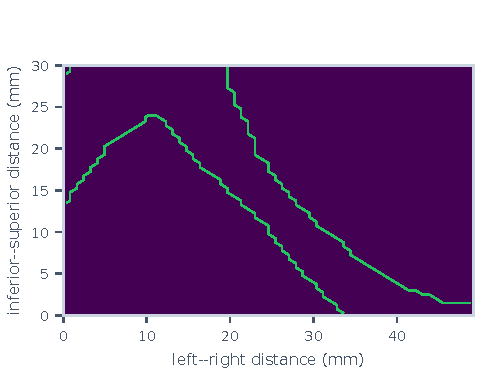
\includegraphics[width=\linewidth]{Figures/pdf/methods/cldice/soft_erosion_depth_10.pdf}
    \caption{Depth 10.}
  \end{subfigure}\hfill
  \begin{subfigure}[t]{0.32\textwidth}
    \centering
    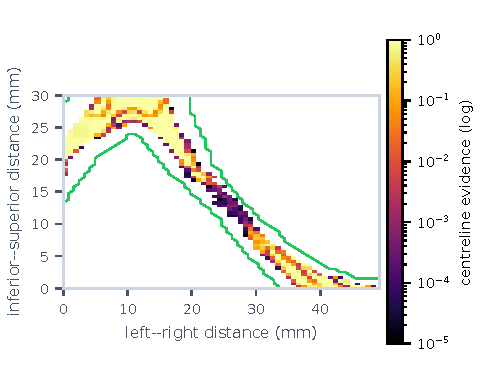
\includegraphics[width=\linewidth]{Figures/pdf/methods/cldice/soft_skeleton_accumulated.pdf}
    \caption{Accumulated $S(p_T)$.}
  \end{subfigure}
  \caption[Extended soft-erosion sequence]{Extended soft-erosion sequence for the real
  airway patch, taken from the final fold-0 EMA teacher. Repeated directional
  minimum pooling removes successive tube layers; ridge residuals extracted at depths
  0--10 are combined into the final graded soft skeleton.}
  \label{fig:soft-skeleton-extended}
\end{figure}

\section{Metric definitions and edge cases}

\begin{itemize}
  \item Pseudocode for native and connected scoring, tree-length detection, branch parsing,
  topology precision and the corrected hard clDice.
  \item Truth table for empty prediction, empty target, both empty, and non-empty disjoint
  trees; document the corrected behaviour and the exact magnitude by which it changed a
  previously reported baseline mean.
  \item Define 6- and 26-neighbour connectivity, the trachea-seed window construction from
  the affine, and the largest-component fallback rule.
  \item Record the ground-truth support inconsistency across historical scoring paths, which
  cases it affects, and the rescoring policy applied before the final tables.
  \item State explicitly why the legacy wall-shell distance bin is excluded from anatomical
  claims, so a reader encountering it in the repository is not misled.
  \item Official-evaluator parity results when complete.
\end{itemize}

\section{Training and inference configurations}

\begin{itemize}
  \item Table of all reportable runs: semantic run name, data, pool, fold, architecture,
  patch, sampling, objective, warm-up and ramp, optimiser, schedule, epochs, checkpoint
  selector and inference settings.
  \item nnU-Net plan summary: target spacing, median image size, patch size, batch size,
  normalisation, deep supervision and mirroring status, ensemble membership.
  \item Full online augmentation specification with per-transform probabilities and ranges,
  plus the additional student perturbation amplitudes and their start epoch.
  \item Exposure arithmetic worked through for each arm: steps per epoch, epochs, total
  labelled and unlabelled patch presentations, per-case draws, and distinct cases sampled per
  epoch.
  \item Hardware and software table: GPU, CUDA, PyTorch, MONAI, nnU-Net versions, operating
  system, git commit, approximate training and inference wall-clock time, and resume history
  for any run that exceeded its walltime.
\end{itemize}

\section{Extended results for the main study}

\begin{itemize}
  \item Per-case tables for every matched pair, with paired differences and bootstrap
  intervals.
  \item Native versus connected audits at 6- and 26-neighbour connectivity, including the
  fragmentation-sensitive cases and the retained-foreground fractions.
  \item Full parsed diagnostic series behind the mid-training measurements: gradient
  contribution and cosine per epoch, teacher evidence statistics, counterfactual losses and
  the objective decomposition. The body reports summary statistics; the appendix carries the
  series and states the sampling frequency.
  \item Checkpoint comparison across all arms under one policy, with the alternative policy as
  a full sensitivity table.
  \item Offline pseudo-labelling per-case differences.
  \item AeroPath per-case table and representative failures once the external test is run.
  \item Deduplicated score inventory for the nnU-Net arms this dissertation reports
  (Table~\ref{tab:nnunet-all-scores}), so that any number quoted in the body can be traced back
  to a single score file.
\end{itemize}

Table~\ref{tab:nnunet-all-scores} collects every arm the body relies on, together with the
reference rungs it is measured against. It reports cohort means only; per-case
values are in the tables above. One score file was selected per prediction directory --- the most
recent complete \texttt{hard-cldice-v2} evaluation at six-neighbour connectivity, falling back to
the original single-connectivity report where no rescored file exists --- and prediction
directories whose means agree to full double precision were collapsed to a single row. The
supervised @110 predictions are the only such collision: two directories hold the same masks under
different names, and appear once here.

\begin{table}[htbp]
  \centering
  \footnotesize
  \setlength{\tabcolsep}{3pt}
  \caption[Deduplicated nnU-Net scores on the frozen external cohorts]{Cohort-mean scores for
  each reported nnU-Net arm, on the native (RAW) mask and after trachea-seeded
  six-neighbour largest-connected-component selection (LCC-6). Dice and precision are voxel-wise;
  TLD is tree length detected and BD is branch detected. All ATM'22 rows use the frozen external
  VAL-20 cohort \{016, 027, 028, 033, 034, 043, 044, 046, 056, 068, 078, 081, 087, 116, 125, 126,
  147, 150, 151, 152\}; the final row is the AeroPath out-of-distribution cohort and shares no
  cases with it. RAW is the primary output and LCC-6 is a sensitivity, not a competing headline.}
  \label{tab:nnunet-all-scores}
  \begin{tabular}{llcrrrrrrrr}
    \toprule
    & & & \multicolumn{4}{c}{RAW (native)} & \multicolumn{4}{c}{$+$ trachea-LCC-6} \\
    \cmidrule(lr){4-7} \cmidrule(lr){8-11}
    Run & Dir. & $n$ & Dice & TLD & BD & Prec. & Dice & TLD & BD & Prec. \\
    \midrule
    \multicolumn{11}{l}{\itshape Supervised nnU-Net, 110 labelled cases (full volume)} \\
    \quad No deep supervision/no mirroring, fold~0 & \texttt{111\_nods\_f0} & 20 & 0.925 & 0.933 & 0.882 & 0.949 & 0.925 & 0.917 & 0.859 & 0.953 \\
    \quad Stock 5-fold ensemble $+$ TTA & \texttt{111\_5f} & 20 & 0.926 & 0.938 & 0.890 & 0.944 & 0.926 & 0.926 & 0.870 & 0.947 \\
    \addlinespace
    \multicolumn{11}{l}{\itshape Supervised and offline-SSL controls, 20 labelled cases (full volume)} \\
    \quad Dice fold~0* & \texttt{120\_dice} & 20 & 0.924 & 0.914 & n/a & 0.934 & 0.919 & 0.875 & 0.798 & 0.942 \\
    \quad clDice fold~0* & \texttt{120\_cldice} & 20 & 0.923 & 0.920 & n/a & 0.927 & 0.916 & 0.883 & 0.810 & 0.933 \\
    \quad Offline pseudo-label SSL & \texttt{121} & 20 & 0.921 & 0.899 & n/a & 0.943 & 0.921 & 0.879 & 0.782 & 0.945 \\
    \addlinespace
    \multicolumn{11}{l}{\itshape Historical ignore-label Mean Teacher, 20 labelled + 90 unlabelled (full volume)} \\
    \quad Cold start & \texttt{122} & 20 & 0.810 & 0.423 & n/a & 0.859 & 0.818 & 0.387 & 0.315 & 0.890 \\
    \quad Warm start, symmetric\textsuperscript{\ddag} & \texttt{122\_sym} & 20 & 0.923 & 0.948 & n/a & 0.922 & 0.926 & 0.922 & 0.876 & 0.937 \\
    \quad Warm symmetric, lung-ROI inference\textsuperscript{\ddag} & \texttt{122\_sym\_roi} & 20 & 0.923 & 0.948 & 0.903 & 0.923 & 0.926 & 0.922 & 0.876 & 0.937 \\
    \addlinespace
    \multicolumn{11}{l}{\itshape Supervised lung-crop seed, 16 labelled cases} \\
    \quad Seed, fold~0 & \texttt{123\_f0} & 20 & 0.922 & 0.913 & 0.834 & 0.928 & 0.926 & 0.895 & 0.814 & 0.940 \\
    \quad Seed, 5-fold ensemble & \texttt{123\_5f} & 20 & 0.923 & 0.915 & 0.840 & 0.937 & 0.927 & 0.901 & 0.823 & 0.947 \\
    \addlinespace
    \multicolumn{11}{l}{\itshape Corrected two-stream arms, 16 labelled + 90 unlabelled (lung crop)} \\
    \quad No-consistency control (final)* & \texttt{124\_ctrl} & 20 & 0.925 & 0.916 & 0.845 & 0.943 & 0.917 & 0.876 & 0.803 & 0.949 \\
    \quad MT90 symmetric (final teacher)* & \texttt{124\_mt\_fin} & 20 & 0.926 & 0.943 & 0.897 & 0.927 & 0.919 & 0.909 & 0.858 & 0.935 \\
    \quad MT90 symmetric (best teacher) & \texttt{124\_mt\_best} & 20 & 0.926 & 0.942 & 0.888 & 0.927 & 0.930 & 0.928 & 0.869 & 0.941 \\
    \quad Offline pseudo-label two-stream* & \texttt{125} & 20 & 0.926 & 0.915 & 0.839 & 0.944 & 0.919 & 0.878 & 0.795 & 0.948 \\
    \addlinespace
    \multicolumn{11}{l}{\itshape Mean Teacher MT240, 16 labelled + 240 unlabelled (lung crop)} \\
    \quad No-consistency control, fold~0 (final)* & \texttt{126\_ctrl} & 20 & 0.926 & 0.920 & 0.855 & 0.936 & 0.922 & 0.884 & 0.813 & 0.946 \\
    \quad K1 fold~0 (final teacher)* & \texttt{126\_K1\_fin} & 20 & 0.925 & 0.938 & 0.884 & 0.941 & 0.920 & 0.905 & 0.848 & 0.949 \\
    \quad K1 fold~0 (best teacher)* & \texttt{126\_K1\_best} & 20 & 0.923 & 0.942 & 0.891 & 0.933 & 0.922 & 0.909 & 0.854 & 0.951 \\
    \quad 5-fold ensemble (final teacher) & \texttt{126\_5f\_fin} & 20 & 0.931 & 0.939 & 0.890 & 0.951 & 0.932 & 0.924 & 0.871 & 0.958 \\
    \quad 5-fold ensemble (best teacher) & \texttt{126\_5f\_best} & 20 & 0.929 & 0.940 & 0.890 & 0.949 & 0.931 & 0.926 & 0.873 & 0.957 \\
    \quad Soft-clDice consistency, fold~0 (final teacher)* & \texttt{126\_softcl\_fin} & 20 & 0.923 & 0.940 & 0.891 & 0.941 & 0.916 & 0.904 & 0.851 & 0.949 \\
    \quad Soft-clDice consistency, fold~0 (best teacher)* & \texttt{126\_softcl\_best} & 20 & 0.922 & 0.940 & 0.891 & 0.937 & 0.917 & 0.904 & 0.849 & 0.946 \\
    \quad Soft-clDice consistency, 5-fold (final teacher) & \texttt{126\_softcl\_5f\_fin} & 20 & 0.928 & 0.938 & 0.889 & 0.946 & 0.931 & 0.925 & 0.872 & 0.955 \\
    \addlinespace
    \multicolumn{11}{l}{\itshape External out-of-distribution evaluation (AeroPath, 27 cases)} \\
    \quad MT240 5-fold ensemble (final teacher) & \texttt{126\_aero} & 27 & 0.845 & 0.951 & 0.924 & 0.845 & 0.841 & 0.920 & 0.896 & 0.855 \\
    \quad Soft-clDice MT240, 5-fold ensemble (final teacher) & \texttt{126\_softcl\_5f\_aero} & 27 & 0.849 & 0.954 & 0.927 & 0.847 & 0.846 & 0.925 & 0.902 & 0.857 \\
    \bottomrule
  \end{tabular}

  \medskip
  \begin{minipage}{\textwidth}
    \footnotesize
    \textbf{Dir.} abbreviates the prediction directory
    \texttt{data/nnunet/predict\_out/Dataset<n>\_...}\ that holds the mask and its score file.
    \textbf{*} marks a run in which case ATM\_044 suffers a connected-component fracture: a short
    bronchial break of roughly 8--15\,mm leaves the left tree detached, so trachea-seeded LCC-6
    deletes it. In every starred run the case retains
    only about 70\,\% of its raw foreground and its tree-length detection falls from roughly 0.98
    raw to 0.58 connected, which is enough on its own to move the LCC-6 cohort mean by more than
    the treatment effects being compared. This is the evidence behind the RAW-primary reporting
    policy, and no arm was selected or tuned to avoid it.
    \textbf{\ddag} These are two separate prediction sets, not a duplicated row; whole-volume and
    lung-ROI-restricted inference agree to three decimal places for the symmetric arm, and differ
    only in the fourth (RAW Dice 0.9228 versus 0.9234).
    \textbf{n/a} indicates that branch metrics were not computed in that score file; the mask exists
    and can be rescored.
  \end{minipage}
\end{table}

\section{Exploratory AeroPath branch-depth profile}
\label{sec:aeropath-depth}

The fold-0 checkpoint difference was negative at depths 0--2 on AeroPath, crossed zero at
depth 3 and reached $+0.0072$ in the pooled $6+$ tail. The five-fold ensemble achieved 0.9593
recovery in that tail, compared with 0.9546 for fold~0 and 0.9474 for the control. This supports
the distal localisation out of domain, but remains exploratory rather than a replicated
training-run effect.

\begin{figure}[htbp]
  \centering
  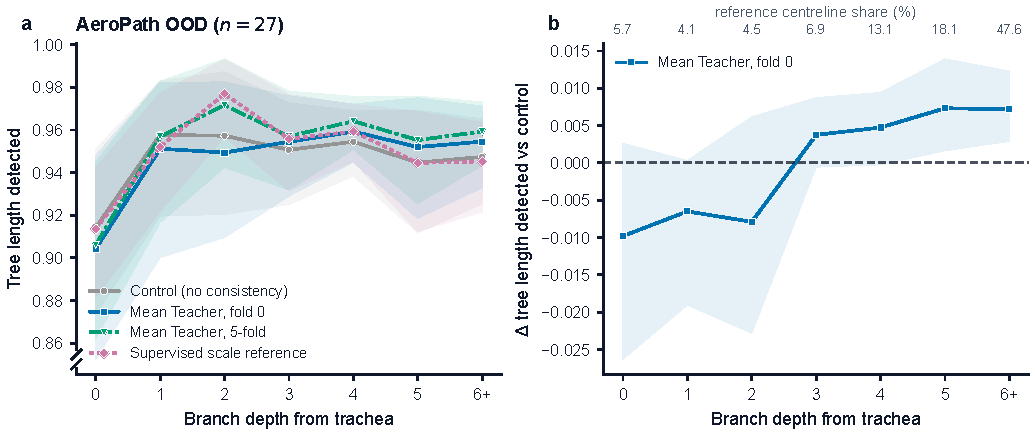
\includegraphics[width=\linewidth]{Figures/pdf/appendix/generation_depth_recovery_aeropath.pdf}
  \caption[AeroPath recovery by branch depth]{Exploratory AeroPath branch-depth recovery.
  (a)~Absolute profiles; (b)~fold-0 Mean Teacher minus control. Depths $\geq6$ are pooled to
  retain all 27 cases. Parser-labelled support excludes 0.25\% of the plain centreline.}
  \label{fig:aeropath-depth}
\end{figure}

\section{Branch depth against airway calibre}
\label{sec:depth-calibre}

The calibre and depth analyses of Sections~\ref{sec:calibre} and~\ref{sec:depth} localise the
same gain along two coordinates, and Figure~\ref{fig:depth-calibre} says how far those
coordinates are the same one. They are related but not interchangeable. The proximal tree is
almost entirely thick: three quarters of the centreline length at depth zero exceeds sixteen
voxels. From depth four onwards the three-to-four-voxel band holds more than half the tree at
every remaining depth, and the narrowest band takes a growing share of the rest, from 8\% at
depth four to a third at the deepest annotated level. Over the reference centreline the two
coordinates rank-correlate at Spearman $\rho=-0.48$; this is a descriptive statistic over
centreline voxels rather than over patients, so no $p$-value is quoted for it. Depth therefore
predicts calibre only loosely, and neither section is a restatement of the other.

\begin{figure}[htbp]
  \centering
  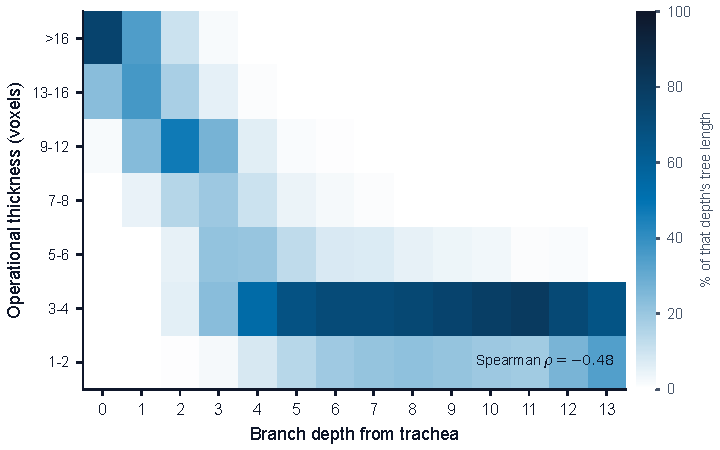
\includegraphics[width=0.86\linewidth]{Figures/pdf/appendix/depth_calibre_heatmap.pdf}
  \caption[Joint distribution of branch depth and airway calibre]{Distribution of reference
  centreline length over operational calibre within each branch depth, on the external
  validation cohort. Each column is normalised to that depth's own tree length, so colour
  reads as the calibre composition of the tree at that depth rather than as its size.}
  \label{fig:depth-calibre}
\end{figure}

\section{Preliminary from-scratch study (superseded)}

% This entire section is material REMOVED from the body during the 2026-08-14 rewire. It is
% retained because the runs happened and the repository contains them, and because a reader
% of the code should be able to reconcile what they find with what the body claims. It is
% NOT part of the dissertation's argument. Keep it descriptive and clearly time-stamped, and
% do not let any body chapter cite a number from here as evidence.

\begin{itemize}
  \item Purpose statement, written defensively: an earlier phase of the project trained a
  from-scratch 3D U-Net under a fixed low-label budget to explore topology-aware objectives
  before a self-configuring pipeline was adopted. It is reported for completeness and to
  document the pivot, not as evidence for any claim in the body.
  \item Configuration: MONAI 3D U-Net, channels $[32,64,128,256,512]$, four stride-2 stages,
  two residual units per level, instance normalisation, PReLU, dropout 0.1; $96^3$ patches,
  foreground-centred sampling probability 0.7, AdamW at $3\times10^{-4}$ with cosine decay and
  mixed precision.
  \item Objective: weighted cross-entropy plus soft Dice, with topology terms withheld for 15
  epochs and ramped over the following 10.
  \item Sealed-test result at validation-fixed thresholds (baseline 0.70, topology variants
  0.50), connected output: baseline hard clDice 0.383, TLD 0.289, topology precision 0.587,
  Dice 0.645, BD 0.229; centreline-loss variant 0.656, 0.592, 0.753, 0.517, 0.451; combined
  centreline plus radius-aware variant 0.709, 0.612, 0.860, 0.560, 0.467.
  \item State the one durable observation and stop there: overlap ranking and tree-completeness
  ranking disagreed sharply in that low-label regime --- the highest-Dice model recovered the
  least reference tree.
  \item State the reason it is superseded, plainly: a supervised nnU-Net trained on the same
  data exceeded these models on every axis including the topology metrics, so absolute airway
  quality in that study was pipeline-bound rather than loss-bound. That result is what
  motivated moving the entire study onto nnU-Net.
  \item Note the post-processing dependence that makes those numbers hard to compare forward:
  at the operating threshold the connected component carried most of the final overlap score
  for the centreline-loss model.
\end{itemize}

\section{Retired ablations (from-scratch pipeline)}

% All negative or inert. Kept as a compact record so the repository is legible and so the
% Discussion can say "these levers were tested" without spending body words on them.

\begin{itemize}
  \item \textbf{Larger patches.} $96^3$ to $128^3$ at otherwise matched settings regressed
  topology (hard clDice 0.683 to 0.334; TLD 0.608 to 0.224) while raising connected Dice
  0.518 to 0.616. The model became conservative rather than sharper. Negative as run, with
  unretuned sampling and epoch count as the stated caveat.
  \item \textbf{Reduced downsampling.} An architecture with a higher-resolution bottleneck
  reproduced the same trade almost exactly: hard clDice 0.516, TLD 0.430, connected Dice
  0.624. Two independent routes to more spatial fidelity both traded tree completeness for
  cleaner proximal masks.
  \item \textbf{Radius-aware objective.} Reduced dependence on connected-component
  post-processing substantially, but at matched tree completeness the final connected masks
  were tied with the centreline-only model, and the geometry-corrected version did not improve
  the balanced model. Retired as a forward lever.
  \item \textbf{Distal sampling and calibre weighting.} Behaved as over-painting rather than
  additional reach; failed their pre-specified decision rules.
  \item \textbf{Gap-bridging reconnection.} Changed tree-length and clDice only at noise scale
  at the tested gap size; the material deleted by connected-component selection was
  predominantly false-positive over-segmentation rather than orphaned true tree.
  \item \textbf{Early semi-supervised arms.} Record the sampler fault --- uniform case
  sampling made all-ignore cases produce batches with no supervised gradient during a long
  warm-up --- and state that the affected arm is excluded from all comparisons as an
  implementation failure rather than a scientific result. Record likewise the loss-ablation
  run truncated at epoch 319 of 1000, whose external score is an early-checkpoint snapshot.
  \item Frame the set honestly in one closing line: these constrain the mechanism by showing
  which levers did not move the completeness/precision frontier, and they informed the
  decision to attack the problem from the data side rather than the loss side.
\end{itemize}

\section{Reproducibility checklist}

\begin{itemize}
  \item Repository layout and exact commands for preprocessing, training, prediction and
  scoring; no machine-specific paths or credentials.
  \item Checksums for final checkpoints, split manifests, prediction bundles and score files;
  note the trainer-source hash pinning used by the launch guards.
  \item Document the known provenance gap --- generated prediction metadata does not record
  trainer, folds or checkpoint filename --- and the convergent evidence used to establish
  checkpoint provenance for affected historical prediction sets.
  \item Unit and integration test summary, including geometry, scoring, ignore-label and
  two-stream provenance tests, plus known deviations from deterministic execution.
  \item Data-access instructions and licence constraints; no redistribution of source scans
  where prohibited.
\end{itemize}

\section{Additional ethical analysis}

\begin{itemize}
  \item Map the main-text discussion onto the six required domains explicitly: scientific
  integrity, collegiality, human subjects, animal welfare, institutional integrity and social
  responsibility --- so the mapping is auditable even where the body text is compressed.
  \item Dataset provenance, licences and source approvals in full.
  \item Extended stakeholder analysis, and the compute/environmental accounting summarised in
  the body.
\end{itemize}

\section{Paired significance tests}

Every significance claim in Chapter~\ref{ch:results} resolves to a row of
Table~\ref{tab:paired-tests}. Because each cohort is scored per case, all comparisons are
paired by case identifier: the statistic is a two-sided paired $t$-test of the per-case
differences against zero, $t=\bar d/(s_d/\sqrt n)$ with $\mathrm{df}=n-1$. Five metrics are
tested per contrast, so a Bonferroni-adjusted $p$-value is given alongside the raw one and
\emph{the adjusted column is what licenses the word significant}. The paired $t$ assumes
approximately normal differences, which is not guaranteed for bounded metrics at $n=20$; a
distribution-free Wilcoxon signed-rank $p$ is therefore reported beside it, and where the two
disagree the Wilcoxon result is the one to quote. Cohen's $d_z=\bar d/s_d$ gives the paired
effect size, and the final column counts cases favouring the arm over its reference.

A limitation applies to every row and is stated once here: these tests quantify consistency
\emph{across patients}, not across training runs. Each arm is a single training run at a
single seed, so a unanimous win count shows that an effect is diffuse rather than carried by
one or two cases; it does not establish that retraining at another seed would reproduce it.

% The complete table environment is generated: \input inside a tabular alignment is a TeX
% error ("Missing \cr inserted"), so the script emits caption, label and all. Re-run
% dissertation/scripts/statistics/paired_significance_tests.py to update it; never hand-edit.
% GENERATED by dissertation/scripts/statistics/paired_significance_tests.py.
% Do not edit: re-run the script so the table and the data stay in agreement.
\begin{table}[htbp]
  \centering
  \scriptsize
  \setlength{\tabcolsep}{3pt}
  \caption[Paired significance tests for every claimed comparison]{Paired
  significance tests for every comparison claimed in this dissertation, on the native
  (RAW) mask. $\bar d$ is the mean per-case difference, arm minus reference. Stars mark
  the Bonferroni-adjusted $p$: ${*}\,p<0.05$, ${**}\,p<0.01$, ${***}\,p<0.001$.
  Generated by \texttt{dissertation/scripts/statistics/paired\_significance\_tests.py}.}
  \label{tab:paired-tests}
  \begin{tabular}{lrcrrrrrrr}
    \toprule
    Metric & $\bar d$ & 95\% CI & $t$ & df & $p$ & $p_{\text{adj}}$ & Wilcoxon & $d_z$ & wins \\
    \midrule
    \multicolumn{10}{l}{\itshape development: probability target vs no-consistency control} \\
    \quad Dice & $-0.0039$ & $[-0.0077,\,-0.0001]$ & $-2.17$ & 19 & $0.0428$ & $0.2139$ & $0.0441$ & $-0.49$ & 7/20 \\
    \quad TLD & $+0.0196$ & $[+0.0147,\,+0.0245]$ & $+8.42$ & 19 & $<\!10^{-4}$ & $<\!10^{-4}$*** & $<\!10^{-4}$ & $+1.88$ & 20/20 \\
    \quad BD & $+0.0362$ & $[+0.0232,\,+0.0491]$ & $+5.84$ & 19 & $<\!10^{-4}$ & $<\!10^{-4}$*** & $<\!10^{-4}$ & $+1.31$ & 19/20 \\
    \quad Prec. & $+0.0057$ & $[-0.0015,\,+0.0129]$ & $+1.66$ & 19 & $0.1129$ & $0.5647$ & $0.1536$ & $+0.37$ & 13/20 \\
    \quad clDice & $-0.0012$ & $[-0.0065,\,+0.0041]$ & $-0.48$ & 19 & $0.6376$ & $1.0000$ & $0.7012$ & $-0.11$ & 9/20 \\
    \addlinespace
    \multicolumn{10}{l}{\itshape development: thresholded target, 5 folds vs no-consistency control} \\
    \quad Dice & $+0.0041$ & $[-0.0053,\,+0.0134]$ & $+0.91$ & 19 & $0.3738$ & $1.0000$ & $0.0897$ & $+0.20$ & 14/20 \\
    \quad TLD & $+0.0190$ & $[+0.0152,\,+0.0228]$ & $+10.47$ & 19 & $<\!10^{-4}$ & $<\!10^{-4}$*** & $<\!10^{-4}$ & $+2.34$ & 20/20 \\
    \quad BD & $+0.0348$ & $[+0.0232,\,+0.0465]$ & $+6.27$ & 19 & $<\!10^{-4}$ & $<\!10^{-4}$*** & $<\!10^{-4}$ & $+1.40$ & 20/20 \\
    \quad Prec. & $+0.0154$ & $[+0.0035,\,+0.0273]$ & $+2.72$ & 19 & $0.0137$ & $0.0683$ & $0.0002$ & $+0.61$ & 17/20 \\
    \quad clDice & $+0.0051$ & $[+0.0013,\,+0.0090]$ & $+2.80$ & 19 & $0.0115$ & $0.0576$ & $0.0136$ & $+0.63$ & 14/20 \\
    \addlinespace
    \multicolumn{10}{l}{\itshape development: thresholded target, 5 folds vs 110-label supervised} \\
    \quad Dice & $+0.0055$ & $[-0.0020,\,+0.0131]$ & $+1.53$ & 19 & $0.1433$ & $0.7166$ & $0.1231$ & $+0.34$ & 13/20 \\
    \quad TLD & $+0.0059$ & $[+0.0009,\,+0.0109]$ & $+2.45$ & 19 & $0.0241$ & $0.1205$ & $0.0242$ & $+0.55$ & 14/20 \\
    \quad BD & $+0.0079$ & $[-0.0023,\,+0.0181]$ & $+1.62$ & 19 & $0.1228$ & $0.6139$ & $0.1089$ & $+0.36$ & 12/20 \\
    \quad Prec. & $+0.0020$ & $[-0.0119,\,+0.0159]$ & $+0.31$ & 19 & $0.7635$ & $1.0000$ & $0.7841$ & $+0.07$ & 8/20 \\
    \quad clDice & $-0.0004$ & $[-0.0048,\,+0.0040]$ & $-0.21$ & 19 & $0.8353$ & $1.0000$ & $0.6742$ & $-0.05$ & 9/20 \\
    \addlinespace
    \multicolumn{10}{l}{\itshape development: probability target, $\beta{=}2$ vs probability target} \\
    \quad Dice & $-0.0743$ & $[-0.1465,\,-0.0020]$ & $-2.15$ & 19 & $0.0446$ & $0.2228$ & $0.0037$ & $-0.48$ & 5/20 \\
    \quad TLD & $+0.0230$ & $[+0.0108,\,+0.0353]$ & $+3.94$ & 19 & $0.0009$ & $0.0044$** & $<\!10^{-4}$ & $+0.88$ & 18/20 \\
    \quad BD & $+0.0475$ & $[+0.0187,\,+0.0763]$ & $+3.45$ & 19 & $0.0027$ & $0.0133$* & $0.0005$ & $+0.77$ & 16/20 \\
    \quad Prec. & $-0.1357$ & $[-0.2266,\,-0.0448]$ & $-3.12$ & 19 & $0.0056$ & $0.0280$* & $<\!10^{-4}$ & $-0.70$ & 0/20 \\
    \quad clDice & $-0.1823$ & $[-0.2888,\,-0.0757]$ & $-3.58$ & 19 & $0.0020$ & $0.0100$** & $<\!10^{-4}$ & $-0.80$ & 0/20 \\
    \addlinespace
    \multicolumn{10}{l}{\itshape sealed test: probability target vs no-consistency control} \\
    \quad Dice & $-0.0008$ & $[-0.0059,\,+0.0042]$ & $-0.35$ & 19 & $0.7301$ & $1.0000$ & $0.8408$ & $-0.08$ & 10/20 \\
    \quad TLD & $+0.0181$ & $[+0.0126,\,+0.0236]$ & $+6.90$ & 19 & $<\!10^{-4}$ & $<\!10^{-4}$*** & $<\!10^{-4}$ & $+1.54$ & 19/20 \\
    \quad BD & $+0.0379$ & $[+0.0263,\,+0.0495]$ & $+6.85$ & 19 & $<\!10^{-4}$ & $<\!10^{-4}$*** & $<\!10^{-4}$ & $+1.53$ & 19/20 \\
    \quad Prec. & $+0.0104$ & $[+0.0021,\,+0.0187]$ & $+2.64$ & 19 & $0.0163$ & $0.0813$ & $0.0083$ & $+0.59$ & 14/20 \\
    \quad clDice & $-0.0016$ & $[-0.0065,\,+0.0034]$ & $-0.67$ & 19 & $0.5087$ & $1.0000$ & $0.5459$ & $-0.15$ & 8/20 \\
    \addlinespace
    \multicolumn{10}{l}{\itshape sealed test: thresholded target, 5 folds vs no-consistency control} \\
    \quad Dice & $+0.0116$ & $[+0.0051,\,+0.0181]$ & $+3.71$ & 19 & $0.0015$ & $0.0074$** & $<\!10^{-4}$ & $+0.83$ & 16/20 \\
    \quad TLD & $+0.0143$ & $[+0.0097,\,+0.0190]$ & $+6.43$ & 19 & $<\!10^{-4}$ & $<\!10^{-4}$*** & $<\!10^{-4}$ & $+1.44$ & 20/20 \\
    \quad BD & $+0.0300$ & $[+0.0192,\,+0.0407]$ & $+5.85$ & 19 & $<\!10^{-4}$ & $<\!10^{-4}$*** & $0.0002$ & $+1.31$ & 18/20 \\
    \quad Prec. & $+0.0233$ & $[+0.0108,\,+0.0358]$ & $+3.90$ & 19 & $0.0010$ & $0.0048$** & $<\!10^{-4}$ & $+0.87$ & 19/20 \\
    \quad clDice & $+0.0017$ & $[-0.0043,\,+0.0077]$ & $+0.59$ & 19 & $0.5619$ & $1.0000$ & $0.3488$ & $+0.13$ & 13/20 \\
    \addlinespace
    \multicolumn{10}{l}{\itshape sealed test: thresholded target, 5 folds vs 110-label supervised} \\
    \quad Dice & $+0.0067$ & $[-0.0058,\,+0.0193]$ & $+1.12$ & 19 & $0.2749$ & $1.0000$ & $0.4980$ & $+0.25$ & 11/20 \\
    \quad TLD & $+0.0037$ & $[-0.0020,\,+0.0095]$ & $+1.36$ & 19 & $0.1893$ & $0.9466$ & $0.0826$ & $+0.30$ & 14/20 \\
    \quad BD & $+0.0140$ & $[+0.0022,\,+0.0259]$ & $+2.48$ & 19 & $0.0227$ & $0.1133$ & $0.0400$ & $+0.55$ & 15/20 \\
    \quad Prec. & $+0.0145$ & $[-0.0089,\,+0.0379]$ & $+1.29$ & 19 & $0.2110$ & $1.0000$ & $0.7562$ & $+0.29$ & 11/20 \\
    \quad clDice & $-0.0037$ & $[-0.0091,\,+0.0017]$ & $-1.43$ & 19 & $0.1692$ & $0.8459$ & $0.2774$ & $-0.32$ & 8/20 \\
    \addlinespace
    \multicolumn{10}{l}{\itshape sealed test: probability target, $\beta{=}2$ vs no-consistency control} \\
    \quad Dice & $-0.0575$ & $[-0.0883,\,-0.0267]$ & $-3.91$ & 19 & $0.0009$ & $0.0047$** & $<\!10^{-4}$ & $-0.87$ & 0/20 \\
    \quad TLD & $+0.0348$ & $[+0.0265,\,+0.0431]$ & $+8.80$ & 19 & $<\!10^{-4}$ & $<\!10^{-4}$*** & $<\!10^{-4}$ & $+1.97$ & 20/20 \\
    \quad BD & $+0.0654$ & $[+0.0485,\,+0.0822]$ & $+8.14$ & 19 & $<\!10^{-4}$ & $<\!10^{-4}$*** & $<\!10^{-4}$ & $+1.82$ & 20/20 \\
    \quad Prec. & $-0.1097$ & $[-0.1547,\,-0.0646]$ & $-5.10$ & 19 & $<\!10^{-4}$ & $0.0003$*** & $<\!10^{-4}$ & $-1.14$ & 0/20 \\
    \quad clDice & $-0.1503$ & $[-0.2254,\,-0.0752]$ & $-4.19$ & 19 & $0.0005$ & $0.0025$** & $<\!10^{-4}$ & $-0.94$ & 0/20 \\
    \addlinespace
    \multicolumn{10}{l}{\itshape AeroPath: probability target vs no-consistency control} \\
    \quad Dice & $+0.0002$ & $[-0.0068,\,+0.0073]$ & $+0.06$ & 26 & $0.9511$ & $1.0000$ & $0.6964$ & $+0.01$ & 16/27 \\
    \quad TLD & $+0.0057$ & $[+0.0012,\,+0.0102]$ & $+2.59$ & 26 & $0.0155$ & $0.0774$ & $0.0082$ & $+0.50$ & 17/27 \\
    \quad BD & $+0.0132$ & $[+0.0041,\,+0.0222]$ & $+3.00$ & 26 & $0.0059$ & $0.0297$* & $0.0046$ & $+0.58$ & 15/27 \\
    \quad Prec. & $+0.0143$ & $[+0.0035,\,+0.0251]$ & $+2.71$ & 26 & $0.0116$ & $0.0581$ & $0.0017$ & $+0.52$ & 20/27 \\
    \quad clDice & $-0.0232$ & $[-0.0358,\,-0.0107]$ & $-3.81$ & 26 & $0.0008$ & $0.0038$** & $0.0007$ & $-0.73$ & 4/27 \\
    \addlinespace
    \multicolumn{10}{l}{\itshape AeroPath: thresholded target, 5 folds vs 110-label supervised} \\
    \quad Dice & $-0.0043$ & $[-0.0132,\,+0.0046]$ & $-0.99$ & 26 & $0.3293$ & $1.0000$ & $0.3242$ & $-0.19$ & 9/27 \\
    \quad TLD & $+0.0053$ & $[+0.0015,\,+0.0091]$ & $+2.85$ & 26 & $0.0085$ & $0.0423$* & $0.0013$ & $+0.55$ & 23/27 \\
    \quad BD & $+0.0034$ & $[-0.0017,\,+0.0084]$ & $+1.36$ & 26 & $0.1840$ & $0.9198$ & $0.1788$ & $+0.26$ & 11/27 \\
    \quad Prec. & $-0.0177$ & $[-0.0217,\,-0.0137]$ & $-9.00$ & 26 & $<\!10^{-4}$ & $<\!10^{-4}$*** & $<\!10^{-4}$ & $-1.73$ & 1/27 \\
    \quad clDice & $-0.0279$ & $[-0.0356,\,-0.0202]$ & $-7.47$ & 26 & $<\!10^{-4}$ & $<\!10^{-4}$*** & $<\!10^{-4}$ & $-1.44$ & 2/27 \\
    \addlinespace
    \bottomrule
  \end{tabular}
\end{table}


% ---------------------------------------------------------------------------
% SUPPLEMENTARY FIGURES (added 2026-08-21). Every figure here is generated by a
% script under dissertation/scripts/ and carries a provenance record under
% Figures/provenance/. Re-run the named script to update one; never edit a PDF.
%
% They are parked at the END OF THE APPENDIX on purpose. The body is capped at
% twenty figures and tables, the appendix is excluded from that cap, and several
% of these depend on arms that are still training. Promoting one into the body is
% a matter of moving its figure environment into the relevant Results section and
% re-running its script with --pdf-output-dir Figures/pdf/results.
%
% FloatBarrier after each group keeps them in the order they are written rather
% than letting LaTeX reorder a queue of fifteen floats.
% ---------------------------------------------------------------------------
\section{Supplementary figures}
\label{sec:supplementary-figures}

The figures collected here support claims the body states in prose or in a table of means.
They are grouped by what they are evidence for rather than by the order they were produced:
the consistency objective, the position of the arms against supervised scale, the
patient-level distribution of the treatment effect, what the difference looks like on an
airway, and the two behaviours --- component filtering and training-run variation --- that
bound how far the result can be read.

Each is generated from the per-case score files and prediction masks already on disk. The
generating script is named in every caption, and each writes a provenance record under
\texttt{Figures/provenance/} listing the exact prediction directories it read.

\subsection{Consistency objective and supervision scale}
\label{sec:supp-objective}

Section~\ref{sec:ablation-mse} asks whether the gain requires a topology-aware consistency
objective or would follow from unlabelled consistency of any form.
Figure~\ref{fig:supp-objective-val} answers it in the paired form the rest of the chapter
uses: both objectives are shown as differences from the \emph{same} no-consistency
comparator, rather than against each other, so the matched-comparator logic is preserved.

Both objectives are drawn at the same consistency weight, $w_{\max}=0.10$, so the two rows
differ in the consistency distance alone; the weight each arm carries is printed on its own
tick label rather than left to a footnote. The two arms are nonetheless independently
realised training runs, as is the comparator they are both differenced against, so the
figure shows consistency across patients and not across training seeds.

\begin{figure}[htbp]
  \centering
  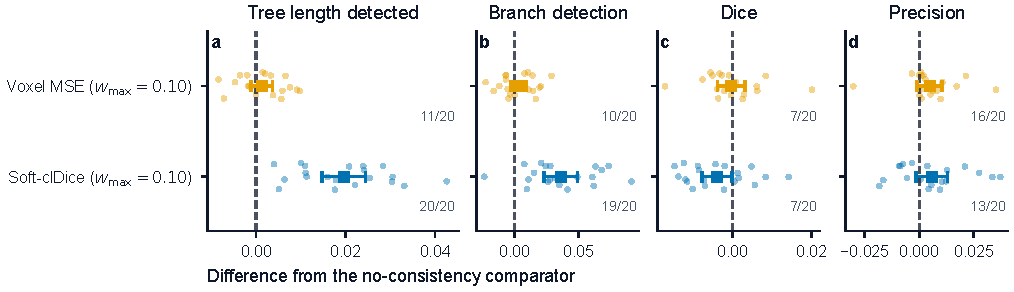
\includegraphics[width=\linewidth]{Figures/pdf/appendix/objective_comparison_val.pdf}
  \caption[Consistency objective, paired against the no-consistency comparator]{Centreline
  against voxelwise consistency on the external validation cohort, each as a paired per-case
  difference from the same no-consistency comparator. Points are patients, squares are means
  with 95\% intervals, and the fraction at the right of each row counts patients favouring
  that arm. Both arms run at $w_{\max}=0.10$: the weight each carries is printed on its own
  label. Both are single training runs, independently realised from the comparator, so this
  is consistency across patients rather than across seeds. Generated by
  \texttt{dissertation/scripts/plot\_arm\_comparison.py}.}
  \label{fig:supp-objective-val}
\end{figure}

\begin{figure}[htbp]
  \centering
  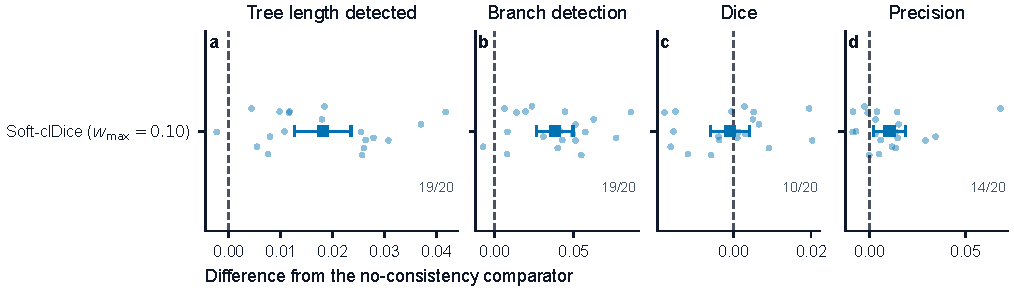
\includegraphics[width=\linewidth]{Figures/pdf/appendix/objective_comparison_test.pdf}
  \caption[Consistency objective on the held-out cohort]{The same contrast on the sealed
  ATM'22 test cohort. Only the centreline objective appears: the voxel-MSE arm has not been
  scored outside the development cohort, and no row is drawn for an arm that has no numbers.}
  \label{fig:supp-objective-test}
\end{figure}

\FloatBarrier

Figure~\ref{fig:supp-scale-val} places the semi-supervised arms against models trained from
larger labelled pools. The shaded rows are a \emph{scale reference} and nothing more. They
differ from the treated arms in labelled-case count, in internal fold membership and in
training protocol at once, so the distance to them is not a label-efficiency measurement,
does not isolate the effect of label count, and is not evidence of equivalence at any point.

\begin{figure}[htbp]
  \centering
  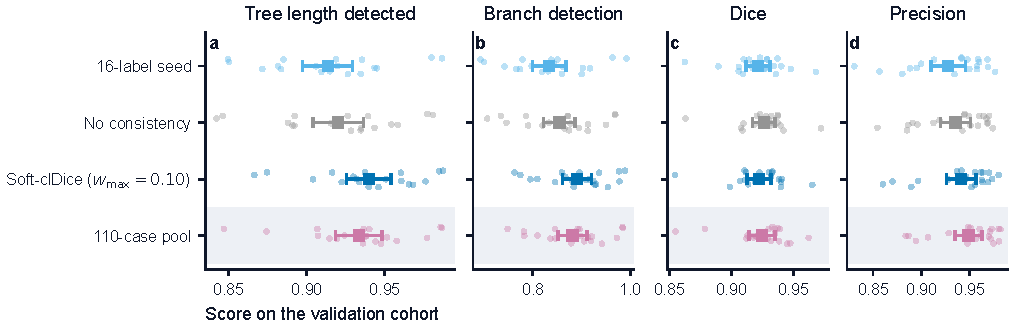
\includegraphics[width=\linewidth]{Figures/pdf/appendix/supervision_scale_val.pdf}
  \caption[Arms against the supervised scale reference, validation cohort]{Per-case scores
  with cohort means and 95\% intervals, external validation cohort. The shaded row is a
  supervised scale reference: it is confounded with fold membership and training protocol,
  so the gap to it is not a matched label-efficiency curve and no equivalence is claimed.
  Generated by \texttt{dissertation/scripts/plot\_arm\_comparison.py}.}
  \label{fig:supp-scale-val}
\end{figure}

\begin{figure}[htbp]
  \centering
  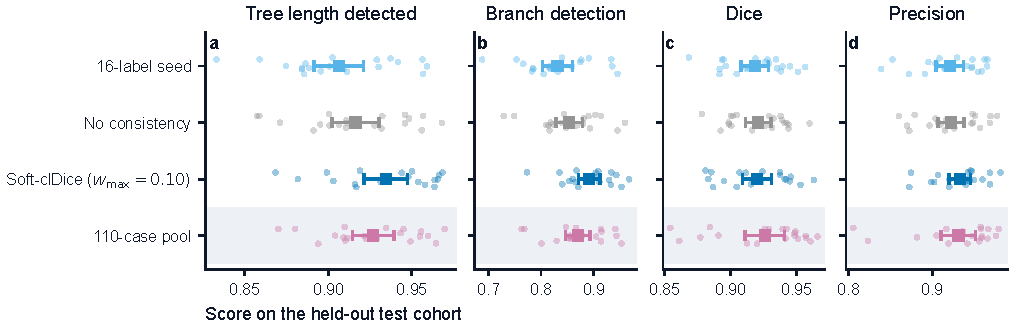
\includegraphics[width=\linewidth]{Figures/pdf/appendix/supervision_scale_test.pdf}
  \caption[Arms against the supervised scale reference, held-out cohort]{The same panel on
  the sealed ATM'22 test cohort. The same caveat applies unchanged.}
  \label{fig:supp-scale-test}
\end{figure}

\FloatBarrier

% Figure~\ref{fig:supp-objective-scale} is the two preceding pairs STACKED. It exists so that
% one slot can carry both arguments if the body ever needs it. Delete it, or delete the four
% figures above it -- do not submit both.
Figure~\ref{fig:supp-objective-scale} stacks the two arguments into a single figure, for the
case where one slot has to carry both. It contains no data the four preceding figures do not.

\begin{figure}[htbp]
  \centering
  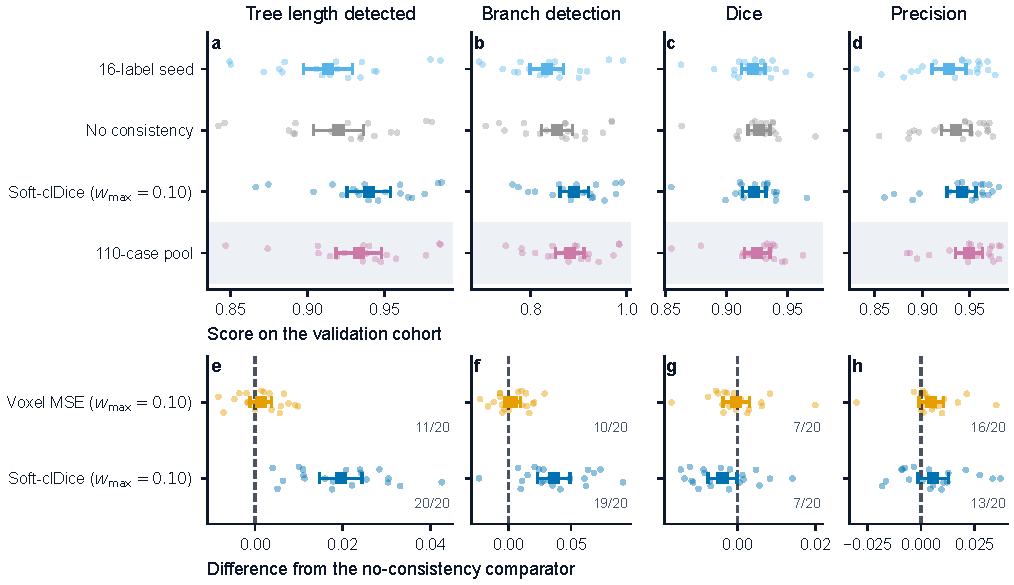
\includegraphics[width=\linewidth]{Figures/pdf/appendix/objective_and_scale_val.pdf}
  \caption[Objective comparison and supervision scale together]{Top row: where each arm sits
  on the external validation cohort, with the supervised scale reference shaded. Bottom row:
  the two consistency objectives as paired differences from the same no-consistency
  comparator. A combined form of Figures~\ref{fig:supp-objective-val}
  and~\ref{fig:supp-scale-val}.}
  \label{fig:supp-objective-scale}
\end{figure}

\FloatBarrier

\subsection{Patient-level treatment effect across cohorts}
\label{sec:supp-paired}

Sections~\ref{sec:primary-matched-pair} and~\ref{sec:external} support two claims with win
counts and cohort means: that the gain is diffuse rather than carried by a few patients, and
that it survives a change of cohort. Both are claims about a \emph{distribution} of paired
differences, which neither a mean nor a win count can show.

Figure~\ref{fig:supp-paired-summary} puts the three cohorts on one axis per metric, so the
effect sizes are compared directly rather than across three tables. AeroPath is drawn beside
the two ATM'22 cohorts but never pooled with them: it is a different scanner and a different
annotation protocol, and the visibly smaller topology difference there is the honest reading
of the out-of-distribution result.

Figure~\ref{fig:supp-paired-cases} then names every patient. All three panels share one
difference axis; the row pitch differs because the cohorts hold different numbers of
patients.

\begin{figure}[htbp]
  \centering
  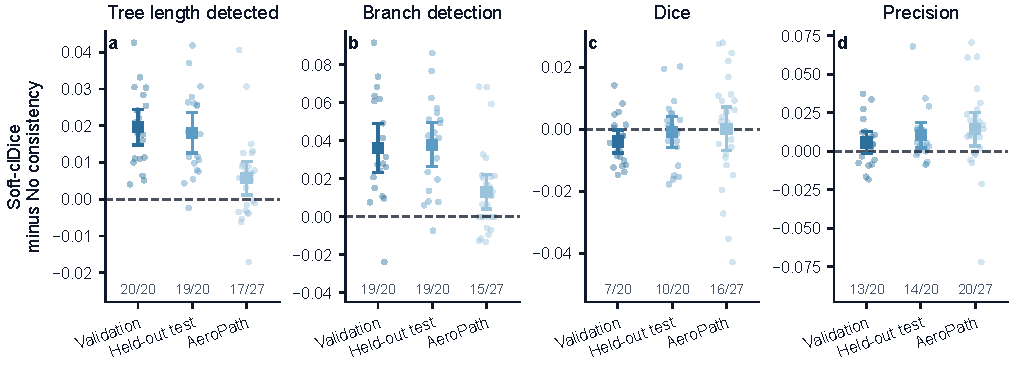
\includegraphics[width=\linewidth]{Figures/pdf/appendix/paired_effect_summary_soft_f0.pdf}
  \caption[Treatment effect by cohort]{Fold-0 Mean Teacher minus its no-consistency
  comparator, on the external validation, sealed test and AeroPath cohorts. Points are
  patients, squares are means with 95\% intervals, and the fraction on the floor of each
  panel counts patients favouring the treatment. Both arms are single training runs, so this
  is consistency across patients, not across seeds. Generated by
  \texttt{dissertation/scripts/plot\_paired\_effects.py}.}
  \label{fig:supp-paired-summary}
\end{figure}

\begin{figure}[htbp]
  \centering
  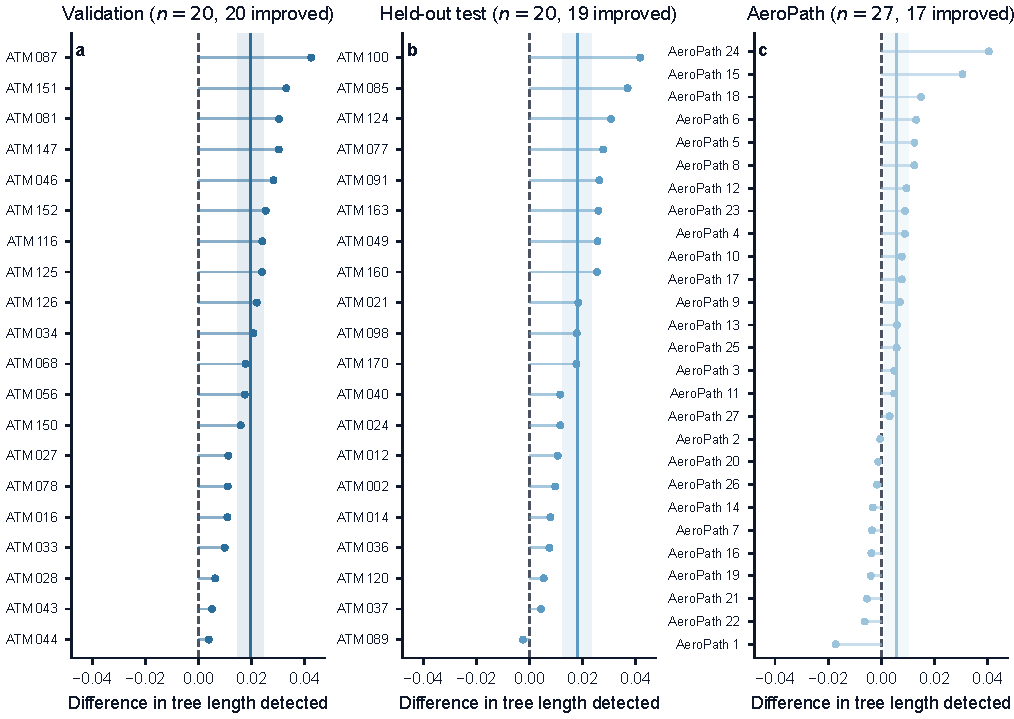
\includegraphics[width=\linewidth]{Figures/pdf/appendix/paired_effect_cases_soft_f0_td_raw.pdf}
  \caption[Per-patient difference in tree length detected]{Every patient's paired difference
  in tree length detected, ordered within each cohort. The vertical line is the cohort mean
  and the band its 95\% interval; all three panels share one difference axis. The
  distribution, not one or two patients, carries the validation and held-out results; on
  AeroPath the effect is smaller and ten of 27 patients fall on the other side of zero.}
  \label{fig:supp-paired-cases}
\end{figure}

\FloatBarrier

\subsection{What the difference looks like on an airway}
\label{sec:supp-qualitative}

A difference of $+0.02$ in tree length detected is not something a reader can picture. The
median-patient render is therefore shown in Figure~\ref{fig:supp-qualitative} in the Discussion,
with supporting cases retained here. Every panel uses the Introduction's isosurface and shading
and one shared screen frame, so the trees overlay pixel for pixel and only the colouring differs.

\textbf{Patients are chosen by a stated rule, never by eye.} Cases are ranked by their own
paired difference in tree length detected, and the rule names a position in that ranking:
Figure~\ref{fig:supp-qualitative} draws the median patient of the validation cohort and
Figure~\ref{fig:supp-error-classes} the largest gain. The complete ranking, including every
patient not drawn, is written to \texttt{Figures/provenance/case\_gallery\_val.json}.

The change panel of Figure~\ref{fig:supp-qualitative} classifies the reference
\emph{centreline}, not reference voxels, because tree length detected is centreline recall:
recovered minus lost, over skeleton length, reproduces the reported paired difference
exactly. A voxel-basis panel would instead be dominated by single-voxel disagreement along
the walls of large airways, which is not what the metric counts.

\begin{figure}[htbp]
  \centering
  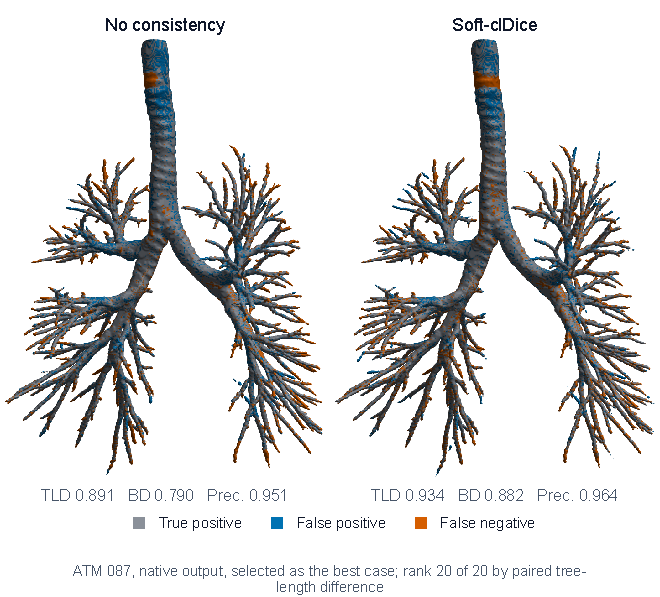
\includegraphics[width=0.65\linewidth]{Figures/pdf/appendix/error_classes_val_control_soft_f0_087.pdf}
  \caption[Voxel error classes for both arms on one patient]{ATM~087, the largest paired
  tree-length gain in the validation cohort, with both arms coloured by voxel error class in
  one shared frame. The distal tips carry the difference: whole terminal branches that are
  false negative under the comparator are produced by the treated arm. The pervasive
  fine-grained false negative along the walls of large airways is wall-thickness
  disagreement, which tree length detected does not count.}
  \label{fig:supp-error-classes}
\end{figure}

\FloatBarrier

\begin{figure}[htbp]
  \centering
  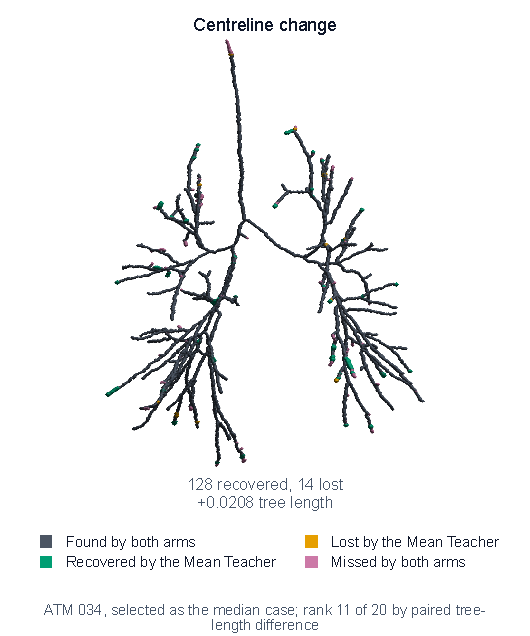
\includegraphics[width=0.52\linewidth]{Figures/pdf/appendix/distal_recovery_val_034.pdf}
  \caption[Distal recovery on the median validation patient]{The change panel of
  Figure~\ref{fig:supp-qualitative} at full width. Recovery is concentrated at the terminal
  branches; the pale class is reference centreline that neither arm produced.}
  \label{fig:supp-recovery-val}
\end{figure}

\begin{figure}[htbp]
  \centering
  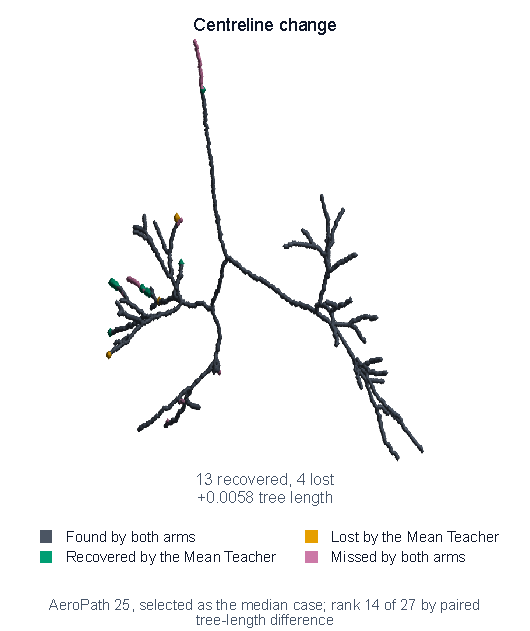
\includegraphics[width=0.52\linewidth]{Figures/pdf/appendix/distal_recovery_ood_925.pdf}
  \caption[Distal recovery out of distribution]{The same panel for AeroPath~25, the median
  patient of that cohort. The annotated tree is shallower than ATM'22's and the change is
  correspondingly smaller: 13 centreline voxels recovered against four lost, a $+0.0058$
  tree-length difference.}
  \label{fig:supp-recovery-ood}
\end{figure}

\FloatBarrier

\subsection{Connected-component filtering and case~044}
\label{sec:supp-postprocessing}

Every metric in this document is reported twice, native and after a trachea-seeded
connected-component filter, and Section~\ref{sec:primary-matched-pair} states in prose that
the filter can delete a detached but genuine subtree. Figure~\ref{fig:supp-postprocessing}
is that statement drawn. The filter is applied by the same function the scorer calls, at the
same connectivity and with the prediction's own affine, so the picture is of the operation
the LCC columns report rather than of a re-implementation.

The two patients are chosen by what the filter did to them: the largest precision gain and
the largest tree-length loss over the cohort. The second rule selects case~044 without being
told to, which is the independent check on the account given in the Discussion.

\begin{figure}[htbp]
  \centering
  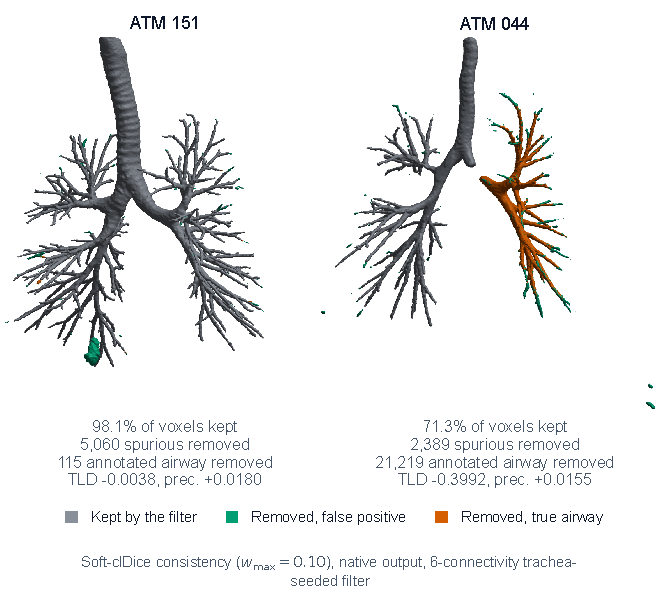
\includegraphics[width=0.65\linewidth]{Figures/pdf/appendix/postprocessing_cases_val_soft_f0.pdf}
  \caption[When component filtering helps and when it deletes airway]{The trachea-seeded
  component filter on two validation patients, each voxel coloured by what the filter did and
  whether it was right to. Left, ATM~151, the largest precision gain in the cohort: the
  filter removes a detached false-positive mass, and 115 annotated airway voxels with it.
  Right, ATM~044: a proximal discontinuity detaches an entire right-lung subtree, and the
  filter deletes 21{,}219 annotated airway voxels, 28.7\% of the prediction, taking tree
  length detected down by $0.3992$. Generated by
  \texttt{dissertation/scripts/render\_postprocessing\_cases.py}.}
  \label{fig:supp-postprocessing}
\end{figure}

\FloatBarrier

\subsection{Training diagnostics}
\label{sec:supp-diagnostics}

Figure~\ref{fig:supp-diagnostics} is descriptive and is labelled as such. The panel that
would matter --- the spread between replicates of one arm, against which the reported
treatment difference has to be read --- requires more than one training run per arm, and the
paired replicate protocol that produces them is still running. The generating script refuses
to draw that panel from a single run and has to be forced past the guard, because a single
trajectory presented as a distribution is precisely the overclaim the protocol exists to
prevent. What is shown instead is one run's optimisation behaviour: the consistency weight
schedule against the gradient it actually produced, and the cosine between the consistency
and supervised gradients.

\begin{figure}[htbp]
  \centering
  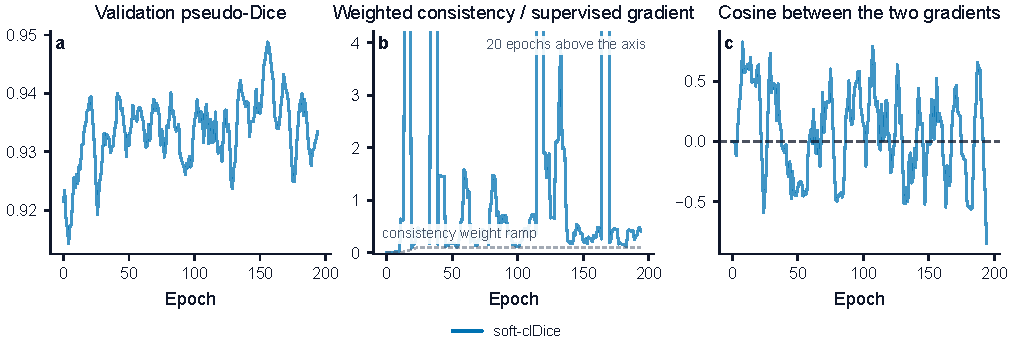
\includegraphics[width=\linewidth]{Figures/pdf/appendix/training_diagnostics_single_run.pdf}
  \caption[Optimisation behaviour of a single Mean Teacher run]{Diagnostics from one
  soft-clDice training run, smoothed with a centred five-epoch mean.
  (a)~nnU-Net's running validation pseudo-Dice.
  (b)~The weighted consistency gradient as a fraction of the supervised one, with the weight
  schedule beneath it; the axis is cut at an interquartile fence and reports how many epochs
  fall above it, all of them steps where the supervised gradient nearly vanished.
  (c)~The cosine between the two gradients, which spends much of training below zero.
  This is a single run and therefore descriptive: it says nothing about run-to-run variation.
  Generated by \texttt{dissertation/scripts/plot\_training\_diagnostics.py}.}
  \label{fig:supp-diagnostics}
\end{figure}

\FloatBarrier

%\include{Appendices/AppendixB}
%TC:endignore

%----------------------------------------------------------------------------------------
%	BIBLIOGRAPHY
%----------------------------------------------------------------------------------------

\printbibliography[heading=bibintoc]

%----------------------------------------------------------------------------------------

\end{document}
